\documentclass[11pt,a4paper]{article}
\usepackage{iftex}
\usepackage[T1]{fontenc}
\usepackage[utf8]{inputenc}
\usepackage{lmodern}
\usepackage[margin=1in]{geometry}
\usepackage{amsmath,amssymb,amsthm,mathtools}
\usepackage{microtype,booktabs,array,enumitem}
\usepackage{flafter}
\usepackage[section]{placeins}
\usepackage[numbers,sort&compress]{natbib}
\usepackage{xcolor,tikz}
\usetikzlibrary{arrows.meta,positioning,calc,patterns}
\definecolor{linkblue}{RGB}{25,60,98}
\usepackage[colorlinks=true,linkcolor=linkblue,citecolor=linkblue,urlcolor=linkblue,
 bookmarksnumbered=true,pdfusetitle,unicode]{hyperref}
\usepackage[nameinlink,capitalise,noabbrev]{cleveref}
\urlstyle{same}
\ifPDFTeX
  \pdfgentounicode=1
  \pdfinfoomitdate=1
  \pdftrailerid{}
  \pdfsuppressptexinfo=15
\fi
\newtheorem{theorem}{Theorem}[section]
\newtheorem{lemma}[theorem]{Lemma}
\newtheorem{proposition}[theorem]{Proposition}
\newtheorem{corollary}[theorem]{Corollary}
\theoremstyle{definition}
\newtheorem{definition}[theorem]{Definition}
\theoremstyle{remark}
\newtheorem{remark}[theorem]{Remark}
\newcommand{\R}{\mathbb R}
\newcommand{\C}{\mathbb C}
\newcommand{\N}{\mathbb N}
\newcommand{\Z}{\mathbb Z}
\newcommand{\dd}{\mathrm d}
\newcommand{\eps}{\varepsilon}
\newcommand{\Id}{\mathrm{Id}}
\DeclareMathOperator{\Op}{Op}
\DeclareMathOperator{\supp}{supp}
\DeclareMathOperator{\tr}{tr}
\DeclareMathOperator{\dist}{dist}
\DeclareMathOperator{\vol}{vol}
\DeclareMathOperator{\diag}{diag}
\DeclareMathOperator{\rank}{rank}
\numberwithin{equation}{section}
\setcounter{tocdepth}{2}
\setlength{\emergencystretch}{2em}
\setlist{topsep=4pt,itemsep=3pt}
\renewcommand{\bibfont}{\raggedright}
\allowdisplaybreaks[2]
\raggedbottom
\clubpenalty=10000
\widowpenalty=10000
\title{Smooth anisotropic uniqueness in the Calder\'on problem\newline from one boundary patch}
\date{}
\begin{document}
\maketitle
\begin{abstract}
We resolve the smooth anisotropic Calder\'on uniqueness problem with
arbitrary same-patch measurements. A smooth Riemannian metric on a compact
connected manifold of dimension at least three is determined, up to a
diffeomorphism fixing the measured patch, by its zero-frequency
Dirichlet-to-Neumann energy form with both input and observation on any
nonempty open boundary patch.
\end{abstract}
{\footnotesize\tableofcontents}
\clearpage
\section{Introduction}
\label{intro:section}

Calder\'on's inverse boundary problem asks whether boundary measurements
determine the coefficients of an elliptic equation. In its geometric
form, the unknown is a Riemannian metric and the measurements are the
Dirichlet energy pairings \eqref{intro:energy} of harmonic extensions.
These pairings are invariant under diffeomorphisms fixing the measured
boundary patch. Theorem~\ref{main:patch} proves uniqueness up to such
diffeomorphisms for smooth metrics in dimension at least three, with
both boundary values and observations on the same open patch.

\subsection{The measurement and the theorem}

Let $M$ be a compact connected smooth $n$-manifold with nonempty smooth
boundary, and let $g$ be a smooth positive-definite Riemannian metric on
$M$, including its boundary. All volume and surface integrals use
densities, so no orientation is required. For $f\in H^{1/2}(\partial M)$,
let $u_f^g\in H^1(M)$ be the unique weak solution of
\[
 -\Delta_g u_f^g=0\quad\text{in }M,\qquad
 u_f^g|_{\partial M}=f.
\]
Here $\Delta_g=\operatorname{div}_g\nabla_g$. For a nonempty relatively
open set $\Gamma\subset\partial M$, put
\[
 H^{1/2}_{co}(\Gamma)
 =\{f\in H^{1/2}(\partial M):\supp f\subset\Gamma\}.
\]
Equip this space with the norm inherited from $H^{1/2}(\partial M)$.
The local energy Dirichlet-to-Neumann map is the bounded operator
\[
 \Lambda_{g,\Gamma}:H^{1/2}_{co}(\Gamma)
       \longrightarrow (H^{1/2}_{co}(\Gamma))^*
\]
defined by
\begin{equation}\label{intro:energy}
 \langle\Lambda_{g,\Gamma}f,h\rangle
 =\int_M\langle\dd u_f^g,\dd u_h^g\rangle_g\,\dd V_g.
\end{equation}
Green's formula gives
\begin{equation}\label{intro:density}
 \langle\Lambda_{g,\Gamma}f,h\rangle
 =\int_\Gamma h\,\partial_{\nu_g}u_f^g\,\dd S_g,
 \qquad f,h\in C_c^\infty(\Gamma),
\end{equation}
where $\nu_g$ is the outward unit normal. In \eqref{intro:density},
$\Lambda_{g,\Gamma}f$ is represented by the density
$\partial_{\nu_g}u_f^g\,\dd S_g$ on $\Gamma$. Each element of
$H^{1/2}_{co}(\Gamma)$ can be approximated in $H^{1/2}(\partial M)$
by smooth functions supported in a fixed compact subset of $\Gamma$
containing its support. By boundedness, equality of
\eqref{intro:energy} on $C_c^\infty(\Gamma)\times C_c^\infty(\Gamma)$
therefore implies equality of the maps on $H^{1/2}_{co}(\Gamma)$.

\begin{theorem}[Smooth anisotropic uniqueness from one patch]
\label{main:patch}
Let $n\ge3$. Let $M$ be a compact connected smooth $n$-manifold with
nonempty smooth boundary, and let $\Gamma\subset\partial M$ be nonempty,
proper, and relatively open. If two smooth Riemannian metrics $g_1,g_2$
on $M$ satisfy
\[
 \Lambda_{g_1,\Gamma}=\Lambda_{g_2,\Gamma},
\]
then there is a smooth diffeomorphism $\Phi:M\to M$, smooth through
the boundary, such that
\[
 \Phi|_\Gamma=\Id,\qquad g_2=\Phi^*g_1.
\]
\end{theorem}

Theorem~\ref{main:patch} allows nonorientable $M$ and disconnected
$\partial M$ or $\Gamma$.

If $\Phi|_\Gamma=\Id$ and $g_2=\Phi^*g_1$, then
$u_f^{g_2}=u_f^{g_1}\circ\Phi$ for $f\in H^{1/2}_{co}(\Gamma)$.
Indeed, the pullback is $g_2$-harmonic and has trace $f\circ\Phi=f$.
Changing variables by $\Phi$ in \eqref{intro:energy} gives
$\Lambda_{g_1,\Gamma}=\Lambda_{g_2,\Gamma}$.

\begin{corollary}[Full-boundary uniqueness]\label{main:full}
Let $M,g_1,g_2$ satisfy the geometric hypotheses of
Theorem~\ref{main:patch}. If the pairings \eqref{intro:energy} for
$\Gamma=\partial M$ agree for all $f,h\in C^\infty(\partial M)$, there
is a smooth diffeomorphism $F:M\to M$ fixing $\partial M$ pointwise
and satisfying $g_1=F^*g_2$.
\end{corollary}

\begin{proof}
For $p\in\partial M$, restrict \eqref{intro:energy} to data supported
in $\Gamma=\partial M\setminus\{p\}$. Theorem~\ref{main:patch} gives
$\Phi|_\Gamma=\Id$. Since $\Gamma$ is dense in $\partial M$,
$\Phi|_{\partial M}=\Id$ by continuity. Take $F=\Phi^{-1}$.
\end{proof}

For the scalar conductivity problem, let
$\Omega\subset\mathbb R^n$ be bounded and connected with smooth
boundary, let $\Gamma\subset\partial\Omega$ be nonempty and relatively
open, and let $\gamma\in C^\infty(\overline\Omega)$ be strictly
positive.  For $f\in C_c^\infty(\Gamma)$, extended by zero to the
rest of the boundary, solve
\[
 \operatorname{div}(\gamma\nabla u_f^\gamma)=0\quad\text{in }\Omega,
 \qquad u_f^\gamma|_{\partial\Omega}=f.
\]
With $\nu_e$ the outward Euclidean unit normal, define the local
conductivity map by
\[
 \Lambda_\gamma^\Gamma f
       =\left.\gamma\partial_{\nu_e}u_f^\gamma\right|_\Gamma.
\]

\begin{corollary}[Smooth scalar uniqueness from one patch]
\label{main:scalar}
Let $n\ge3$, and let $\Omega$ and $\Gamma$ be as above.  If two
strictly positive conductivities
$\gamma_1,\gamma_2\in C^\infty(\overline\Omega)$ satisfy
\[
 \Lambda_{\gamma_1}^\Gamma f=\Lambda_{\gamma_2}^\Gamma f
       \quad\text{for every }f\in C_c^\infty(\Gamma),
\]
then $\gamma_1=\gamma_2$ on $\overline\Omega$.
\end{corollary}

For $g=\gamma^{2/(n-2)}e$, with $e$ the Euclidean metric,
\eqref{scalar:energy-conversion} identifies the conductivity and metric
energies. The proof in Section~\ref{scalar:section} uses this identity
and \eqref{intro:density} to apply Theorem~\ref{main:patch}.
Since $g_2=\Phi^*g_1$, the metric $\Phi^*e$ is conformal to $e$.
Lemma~\ref{scalar:boundary-rigidity} gives $\Phi=\Id$.

\subsection{Historical context}

Calder\'on formulated the inverse conductivity problem through boundary
measurements of Dirichlet energy and studied its linearization
\cite{Calderon1980}. Kohn and Vogelius established scalar boundary
determination \cite{KohnVogelius1984}. Sylvester and Uhlmann proved
full-data uniqueness for smooth scalar conductivities in Euclidean
dimensions at least three using complex geometrical optics solutions
\cite{SylvesterUhlmann1987}. For anisotropic conductivities, Lee and
Uhlmann developed boundary determination and proved real-analytic
recovery under geometric and topological hypotheses
\cite{LeeUhlmann1989}. Lassas and Uhlmann subsequently recovered a
real-analytic manifold and metric from an arbitrary nonempty
real-analytic boundary patch in dimensions at least three, without
the earlier topological restrictions
\cite[Theorem~1.1(ii)]{LassasUhlmann2001}. Their Green-function method
also led to the complete-manifold extension of Lassas, Taylor, and
Uhlmann \cite{LassasTaylorUhlmann2003}. Guillarmou and S\'a Barreto
proved uniqueness for smooth compact Einstein manifolds with the same
Einstein constant from data on one boundary patch. They use the Einstein
equation to recover the metric near that patch and analytic continuation
in the interior \cite[Theorem~1.1]{GuillarmouSaBarreto2009}.

For scalar inverse problems with partial boundary data, Bukhgeim and
Uhlmann introduced a method based on Carleman estimates
\cite{BukhgeimUhlmann2002}. Kenig, Sj\"ostrand, and Uhlmann prescribed
boundary values near the back face and observations near the front
face for a point outside the convex hull
\cite[Theorem~1.1]{KenigSjostrandUhlmann2007}. Their conductivity
corollary also assumes that the two conductivities agree on the
whole boundary \cite[Corollary~1.4]{KenigSjostrandUhlmann2007}.
In dimension three, Isakov used reflection to prove uniqueness from
data on one patch when the rest of the boundary lies in a plane or
sphere \cite{Isakov2007}. For the Schr\"odinger problem linearized at
zero potential, Dos Santos Ferreira, Kenig, Sj\"ostrand, and Uhlmann
proved $L^1$ density of products of harmonic functions whose traces
vanish outside the measured patch
\cite[Theorem~1.1]{DosSantosFerreiraEtAl2009}. Alessandrini and Kim
proved stability from data on one patch for scalar conductivities
known near the whole boundary \cite[Theorem~2.5]{AlessandriniKim2012}.

Smooth geometric results also exploit special backgrounds.
Dos Santos Ferreira, Kenig, Salo, and Uhlmann developed limiting
Carleman weights and recovered potentials and conformal factors on
manifolds conformal to submanifolds of a product of a line and
a simple Riemannian manifold \cite{DSFKSU2009}. Kenig and Salo
extended partial boundary data methods on such products and related
them to geodesic and broken-ray transforms \cite{KenigSalo2013}.

Recent full-data results establish rigidity near prescribed smooth
backgrounds. Lin proves rigidity near the Euclidean metric under
smallness in a H\"older norm \cite[Theorem~1.1]{Lin2026}.
Mu\~noz-Thon and Stefanov prove local rigidity near every smooth
conformally Euclidean metric under Sobolev smallness
\cite[Theorem~2]{Stefanov2026}. Chen, Jiang, Liu, and Tao obtain
uniqueness from data on one patch under quasianalyticity, and for
smooth metrics under additional foliation and one-sided ordering
assumptions
\cite[Corollary~1.2, Theorem~1.6 and Corollary~1.7]{ChenJiangLiuTao2026}.
Theorem~\ref{main:patch} allows arbitrary smooth metrics and any
nonempty proper relatively open patch for both inputs and observations.

Uhlmann and Wang recover compactly supported potentials, and conformal
factors equal to one near the boundary, on a fixed near-Euclidean
three-dimensional metric with strictly convex boundary and an invertible
Dirichlet problem \cite{UhlmannWangNear2026}. Their partial-data result
recovers a potential near the measured boundary in a strictly convex
three-dimensional domain, with the potential supported away from the
measured patch \cite{UhlmannWangPartial2026}.
Daud\'e, Enciso, Helffer, Kamran, and Nicoleau propagate local DN
equality to a whole connected boundary component when the metrics
already agree in a collar of that component
\cite{DaudeEtAlPropagation2026}.

Harmonic functions provide an intrinsic way to describe points and
coordinates. Greene and Wu studied embeddings by harmonic functions
\cite{GreeneWu1975}; the Poisson embedding approach of Lassas,
Liimatainen, and Salo represents a point by its evaluation on
harmonic functions with prescribed boundary values \cite{LLS20}.
They also represent points by evaluations of zero-Dirichlet solutions
with sources in a fixed interior open set, as in
\eqref{data:evaluations}
\cite[Definition~6.1 and Proposition~6.8]{LLS20}. Their Runge
approximation and prescribed harmonic jet results apply to smooth
metrics \cite[Propositions~A.2 and A.5]{LLS20}. Their global continuation
theorem assumes real analyticity \cite[Theorem~3.3]{LLS20}.
Theorem~\ref{local:extension} uses the estimate
\eqref{local:density-bound}, uniform as the spheres shrink, to extend
equality of smooth metrics across a hypersurface.

Runge approximation for elliptic equations goes back to Lax and
Malgrange \cite{Lax1956,Malgrange1956}. R\"uland and Salo proved a
quantitative version for data supported in a boundary patch
\cite{RulandSalo2019}. Lemma~\ref{data:jet-family} obtains the required
second jets by testing distributions supported at a point against
solutions with sources in the cap. Precedents include determination
of the conductivity at the boundary from local data
\cite{AlessandriniGaburro2009} and comparison of Green functions on
an enlarged domain \cite[Sections~3--4]{AlessandriniKim2012}.

\subsection{Proof strategy}

The global argument uses the local metric extension
Theorem~\ref{local:extension}. In two interior harmonic coordinate
charts identified with a neighborhood of $0$, its hypotheses are
$g_1=g_2$ on an open set $W$, equality of the Dirichlet Green kernels
$G_1(x,y)=G_2(x,y)$ for $x,y\in W$ and $x\ne y$, and finitely many
pairs $(u_1^a,u_2^a)$ with $\Delta_{g_j}u_j^a=0$ and $u_1^a=u_2^a$
on $W$. The coordinate Hessians $(\partial_i\partial_j u_1^a(0))$
must span the symmetric matrices $H$ with $g_1^{ij}(0)H_{ij}=0$. If $W$ contains one side of a smooth
hypersurface through $0$, the theorem extends $g_1=g_2$ to a
neighborhood of $0$. Proving this theorem for smooth coefficients
is the main task.

Lemma~\ref{data:jets} recovers the complete boundary jets in
boundary-normal coordinates from equality of the maps in
\eqref{intro:energy}. Proposition~\ref{data:cap} uses these jets to
attach an exterior cap $E$ with $g_1=g_2$ on $E$, and uses
\eqref{intro:energy} to prove $G_1(x,y)=G_2(x,y)$ for $x,y\in E$ and
$x\ne y$. For $f\in C_c^\infty(U_0)$, where $U_0\Subset E$,
the solutions $u_f^j$ defined in \eqref{data:evaluations} then agree
on $E$ by \eqref{data:green-normalization}. Lemma~\ref{data:jet-family}(i)
shows that the evaluations $f\mapsto u_f^j(p)$ distinguish interior
points. Lemma~\ref{data:jet-family}(ii) gives every second jet
satisfying $\Delta_{g_j}u(p)=0$ at interior points outside
$\overline{U_0}$. These functions supply the coordinates and pairs
required by Theorem~\ref{local:extension}.

After the dilation \eqref{cross:dilation}, the kernel
$\mathcal G_\lambda$ in \eqref{cross:mixed-data} satisfies
$\Delta_{g_1(\lambda\cdot),x}\mathcal G_\lambda=
\Delta_{g_2(\lambda\cdot),y}\mathcal G_\lambda=0$ for $x\ne y$.
Proposition~\ref{cross:initial} extends \eqref{cross:mixed-data} to
prescribed compact sets at positive distance from $x=y$. It uses
Lemma~\ref{cross:series}, whose construction by singular functions of
a restriction operator has antecedents in \cite{Zeriahi1982}.
Under \eqref{balls:bootstrap-condition},
Proposition~\ref{balls:continuation} continues $\mathcal G_\lambda$
to neighborhoods of the spheres of radius $r_\delta(y)$ in
\eqref{balls:radius}. The boundary integral \eqref{balls:flux} over
these spheres defines $T_y$. Proposition~\ref{balls:functional} proves
$T_y\bigl(u_1^a(\lambda\cdot)\bigr)=u_2^a(\lambda y)$,
$T_y1=1$, and $T_yx^i=y^i$ in \eqref{balls:reproduction}.

Let $h$ be the difference of normalized inverse metrics in
\eqref{balls:normalization} and
$H_8=\sum_{|\alpha|\le8}|\partial^\alpha h|$. Under the bounds in
\eqref{balls:bootstrap-condition}, Proposition~\ref{balls:functional}
represents $T_y$ by the density $\psi$ in
\eqref{balls:density-representation}, and Lemma~\ref{local:density}
gives the $L^2$ estimate \eqref{local:density-bound} uniformly in
$\delta$. The identities $T_y1=1$ and $T_yx^i=y^i$ in
\eqref{balls:reproduction} allow the affine Taylor polynomial at $y$
to be subtracted in \eqref{balls:density-representation}. With
\eqref{local:density-bound}, Lemma~\ref{local:moment} then obtains the
$L^2$ bound \eqref{local:moment-bound} for the differences of the
functions $\lambda^{-2}v_j^a(\lambda\cdot)$ from
\eqref{local:renormalized-pairs} divided by
$r_\delta^2$, with the cutoff in \eqref{balls:cutoff-region}.
The system \eqref{local:metric-system} determines $h$ from the Hessians
of these differences. Using Lemma~\ref{local:interpolation},
Lemma~\ref{local:improvement} gives $H_8\le Cr_\delta^{3/2}$ in
\eqref{local:superlinear} for small $r_\delta$.

The order of parameter choices is \eqref{local:parameter-order},
with the threshold set by \eqref{local:rho-choice} before the
dilation $\lambda$ is fixed using \eqref{local:one-dilation}.
The proof of Theorem~\ref{local:extension} uses
\eqref{local:superlinear} and the choice of $\lambda$ to improve
$H_8\le\eps r_\delta$ to $H_8\le\eps r_\delta/2$. The initial bound
$H_8\le\eps r_1$ and continuity in $\delta$ give
$H_8\le\eps r_\delta$ for all $0<\delta\le1$. With $\lambda$ fixed,
$r_\delta\to0$ near $0$ by Lemma~\ref{balls:profiles}, so $h=0$ there.
By \eqref{balls:normalization} the metrics are conformal. The harmonic
coordinate equations in the proof of Theorem~\ref{local:extension}
make the conformal factor constant for $n\ge3$, and
$g_1(0)=g_2(0)$ makes it equal to one.

The harmonicity of $T_yu$ in Proposition~\ref{balls:functional}
and the differentiation in Lemma~\ref{angular:trace} give $P\psi=0$
in \eqref{angular:P-equation}.
The decomposition \eqref{angular:P-decomposition} includes the
second-order terms from differentiating the moving spheres.
Proposition~\ref{angular:coercivity} combines the spherical harmonic
estimate \eqref{angular:raising-estimate} of Lemma~\ref{angular:raising}
with \eqref{angular:norm-comparison} and \eqref{angular:error-form-bound}
to prove \eqref{angular:coercive-estimate}. The spherical harmonic
decomposition of tensors also appears in \cite{PSU15,GPSU16}.
Lemma~\ref{local:density} applies \eqref{angular:coercive-estimate}
to $\chi(\psi-1)$ to obtain \eqref{local:density-bound}.

The injectivity of the evaluations in \eqref{data:evaluations},
given by Lemma~\ref{data:jet-family}(i), makes $\Phi$ unique on the
domain where \eqref{global:matching} holds. If $p_k$ tends to an
interior point, any limit of $\Phi(p_k)$ is interior by
\eqref{global:matching} and Lemma~\ref{data:jet-family}(i), since
the evaluations vanish on the boundary and are nonzero in the interior. In Proposition~\ref{global:frontier},
a ball in the domain of $\Phi$ that touches its complement supplies
the open set $W$ for Theorem~\ref{local:extension}. Equality of the
Green kernels on this ball comes from \eqref{global:green-equality}.
Theorem~\ref{local:extension} extends metric equality across the
point of contact. Interior unique continuation as in
Section~\ref{data:section} extends equality of the harmonic functions,
so the extended isometry still satisfies \eqref{global:matching}.
Proposition~\ref{global:completion} extends $\Phi$ smoothly through
the boundary and uses \eqref{intro:density} and boundary unique
continuation from Section~\ref{data:section} to prove $\Phi|_\Gamma=\Id$.

Section~\ref{data:section} constructs the common cap and harmonic
functions from sources in the cap. Section~\ref{cross:section}
states Theorem~\ref{local:extension} and extends
\eqref{cross:mixed-data} at positive distance from $x=y$.
Section~\ref{sec:balls} constructs $T_y$ in \eqref{balls:flux}.
Section~\ref{sec:angular} proves \eqref{local:density-bound}, and
Section~\ref{sec:bootstrap} uses it to prove
Theorem~\ref{local:extension}. Section~\ref{global:section} completes
the proof of Theorem~\ref{main:patch}. Section~\ref{scalar:section}
proves Corollary~\ref{main:scalar}.
\section{Boundary data and a common interior region}
\label{data:section}

From equality of the maps in \eqref{intro:energy}, Lemma~\ref{data:jets}
obtains equality of all boundary metric jets in boundary-normal
coordinates. Proposition~\ref{data:cap} attaches a common exterior
region $E$ and proves $G_1(x,y)=G_2(x,y)$ for $x,y\in E$, $x\ne y$.
Lemma~\ref{data:jet-family} uses solutions with sources in $E$ to
obtain the harmonic coordinates and Hessians in Theorem~\ref{local:extension}.

We write $L_g=-\Delta_g$, where $\Delta_g=\operatorname{div}_g\nabla_g$,
and use Riemannian densities as in \eqref{intro:energy}
and \eqref{intro:density}. On a compact connected smooth manifold with
nonempty boundary, the Poincar\'e inequality on $H^1_0$ makes the
Dirichlet realization $L_{g,D}$ invertible. By Dirichlet regularity,
smooth sources and boundary values give solutions smooth up to the
boundary.

For smooth scalar second-order elliptic operators with real positive
definite principal symbol, a solution that vanishes on one side of a
smooth hypersurface vanishes near it
\citep[Definition~8.2(a) and Theorem~8]{KochTataru2005}.
Applying this across coordinate spheres gives interior unique
continuation. On a connected domain, vanishing on a nonempty open
subset implies vanishing throughout the domain.

If a smooth harmonic function $u$ satisfies $u=\partial_{\nu_g}u=0$
on an open boundary patch, extend the metric smoothly across that
patch and extend $u$ by zero. Both boundary terms of Green's second
identity vanish, so the extension satisfies $\Delta_g u=0$
distributionally across the patch. Interior elliptic regularity
and \citep[Theorem~8]{KochTataru2005} give $u=0$ near the patch and
then throughout the connected interior.

\subsection{The density and the boundary jets}

The surface density $\dd S_g$ in \eqref{intro:density} contributes
to the principal symbol of $\Lambda_{g,\Gamma}$ in the proof of
Lemma~\ref{data:jets}.

\begin{lemma}[Boundary jets]\label{data:jets}
Let $g_1,g_2$ be smooth metrics on a compact connected smooth
$n$-manifold $M$ with nonempty boundary, where $n\ge3$. Suppose
$\Lambda_{g_1,\Gamma}=\Lambda_{g_2,\Gamma}$ for the maps
\eqref{intro:energy} on a nonempty relatively open set
$\Gamma\subset\partial M$. In boundary-normal coordinates for the
respective metrics, based on the same coordinates on $\Gamma$,
their complete boundary Taylor jets agree.
\end{lemma}

\begin{proof}
Fix a boundary chart compactly contained in $\Gamma$, and write $h$
for the matrix of the induced metric there. By \eqref{intro:density}
and the factorization \eqref{data:factorization}, the principal symbol
of $\Lambda_{g,\Gamma}$ relative to $\dd z$ is
\[
 \sqrt{\det h(z)}\sqrt{h^{ab}(z)\xi_a\xi_b}.
\]
Its square determines $(\det h)h^{-1}$, whose determinant is
$(\det h)^{n-2}$. Since $n\ge3$, this determines $\det h$, and hence
$h$. Dividing the equal densities in \eqref{intro:density} by the
common $\dd S_g=\sqrt{\det h}\,\dd z$ gives equality of the maps
$f\mapsto\partial_{\nu_{g_j}}u_f^{g_j}$ on the patch. After localization
by cutoffs supported in $\Gamma$ and equal to one near a chosen point,
these maps have equal full symbols there.

To recover the normal derivatives of $h$, use the symbol recursion
of \citet{LeeUhlmann1989}. In the inward normal coordinate $s\ge0$,
write
\[
 g=ds^2+h(s,z),\qquad
 a=\frac12\tr(h^{-1}\partial_s h),\qquad
 L_g=-\partial_s^2-a\partial_s+P,
\]
where $P=-\Delta_{h(s)}$ acts in $z$. The scalar case of the
factorization in \citep[Proposition~3.1]{JoshiLionheart2005} gives
a tangential pseudodifferential operator $B(s)$ of order one, with
positive principal symbol, satisfying
\begin{equation}\label{data:factorization}
 L_g=(-\partial_s+B-a)(\partial_s+B)
          \pmod{\Psi^{-\infty}},\qquad
 B^2-aB-\partial_sB=P\pmod{\Psi^{-\infty}}.
\end{equation}
The remainders are smoothing in $z$ and smooth in $s$. The local
Poisson parametrix from \citep[Section~3]{JoshiLionheart2005} solves
$(\partial_s+B)u=0$ modulo smoothing terms. Since $\partial_{\nu_g}
=-\partial_s$ at $s=0$, $B(0)$ has the full symbol of
$f\mapsto\partial_{\nu_g}u_f^g$.

For precision, use left symbols and $D_z=-i\partial_z$, so
\[
 b\mathbin{\#}c\sim
 \sum_\alpha\frac{(1/i)^{|\alpha|}}{\alpha!}
       (\partial_\xi^\alpha b)(\partial_z^\alpha c).
\]
Write $b\sim b_1+b_0+b_{-1}+\cdots$ for the symbol of $B$ and
$p=p_2+p_1$ for that of $P$. The second identity in
\eqref{data:factorization} gives
\[
 b_1=\rho=(h^{ab}\xi_a\xi_b)^{1/2},\qquad
 b\#b-ab-\partial_sb=p.
\]
Taking the homogeneous terms of degree one in
\eqref{data:factorization} gives
\[
 2\rho b_0+\frac1i\partial_\xi\rho\cdot\partial_z\rho
             -a\rho-\partial_s\rho=p_1.
\]
Since $P=-\Delta_{h(s)}$, both $p_1$ and
$i^{-1}\partial_\xi\rho\cdot\partial_z\rho$ depend only on $h$ and
its tangential derivatives. Differentiating $\rho^2=h^{ab}\xi_a\xi_b$
gives
\[
 \partial_s\rho
 =-\frac{(\partial_s h)(\xi^\sharp,\xi^\sharp)}{2\rho},
 \qquad \xi^\sharp=h^{-1}\xi.
\]
Using this and $a=\tfrac12\tr(h^{-1}\partial_s h)$, the term of $b_0$
containing $\partial_s h$ is
\[
 \frac14\left(\tr_h\partial_s h
       -\frac{(\partial_s h)(\xi^\sharp,\xi^\sharp)}{\rho^2}\right).
\]
For $k\ge2$, the terms of degree $2-k$ in the symbol equation from
\eqref{data:factorization} express $2\rho b_{1-k}-\partial_s b_{2-k}$
using $a$, $b_1,\ldots,b_{2-k}$, and their tangential derivatives.
These terms involve at most $k-1$ normal derivatives of $h$.
Writing $A_k=\partial_s^k h$, induction from the formula for $b_0$
gives, for $k\ge1$,
\begin{equation}\label{data:highest-jet}
 b_{1-k}=
 \frac{1}{4(2\rho)^{k-1}}
 \left(\tr_h A_k-
        \frac{A_k(\xi^\sharp,\xi^\sharp)}{\rho^2}\right)
 +\text{terms involving }\partial_s^j h\ (j<k).
\end{equation}
The remaining terms may also involve tangential derivatives of
$\partial_s^j h$ with $j<k$.
In the induction step, differentiation of $A_{k-1}$ in
\eqref{data:highest-jet} is the only contribution involving $A_k$.
Division by $2\rho$ gives the displayed factor.

Suppose the two normal jets agree through order $k-1$ as smooth
functions on the boundary chart. Their tangential derivatives also
agree. Equality of the symbols of $B(0)$ and \eqref{data:highest-jet}
give, with $A=\partial_s^k(h_1-h_2)|_{s=0}$,
\[
 \tr_h A-A(v,v)=0,\qquad v=\xi^\sharp/\rho,\quad |v|_h=1.
\]
Polarization gives $A=(\tr_h A)h$. Taking the trace gives
$(n-2)\tr_h A=0$, hence $A=0$. Induction from equality of $h$ at
$s=0$ gives equality of all its normal and mixed derivatives there.
The normal components are $g_{ss}=1$ and $g_{sa}=0$, so the full
metric jets agree.

The calculation uses the local symbols in \eqref{data:factorization}
and the densities in \eqref{intro:density}. It applies to nonorientable
manifolds, and other boundary components affect only the smoothing
terms of the localized operator.
\end{proof}

\subsection{Attaching a common cap}

The boundary jets in Lemma~\ref{data:jets} allow both metrics to be
extended by the same coefficients across a smaller patch of $\Gamma$.
Proposition~\ref{data:cap} uses equality of the maps in
\eqref{intro:energy} to compare the Green kernels on the added region.

\begin{proposition}[Common extension and equality of Green kernels]\label{data:cap}
Under the hypotheses of Lemma~\ref{data:jets}, there are compact
connected smooth extensions $(M_j^e,g_j^e)$ of $(M,g_j)$, with a
common connected open exterior region $E$ on which $g_1^e=g_2^e$. The cap is attached through a nonempty open set
$P_0\Subset\Gamma$. The extended zero-Dirichlet Green kernels satisfy
\[
 G_1(x,y)=G_2(x,y),\qquad x,y\in E,\quad x\ne y.
\]
For every $F\in C_c^\infty(E)$, the solutions of
$-\Delta_{g_j^e}w_j=F$ with zero Dirichlet data on $\partial M_j^e$
satisfy $w_1=w_2$ on $E$.
\end{proposition}

\begin{proof}
Choose a nonnegative smooth function $b$ supported compactly in
a boundary coordinate chart in $\Gamma$, with $P_0=\{b>0\}$
nonempty and connected. Extend the boundary-normal coordinate domains
of Lemma~\ref{data:jets} to $s<0$ and replace $s=0$ by $s=-b(z)$.
Take $b$ sufficiently small that the graph lies in the extended
coordinate domains. The extended manifolds are smooth, compact,
and connected, with common exterior region
\[
 E=\{(z,s):-b(z)<s<0\}.
\]
Extend the coefficients of $g_1$ smoothly to $s<0$. They remain
positive definite in a sufficiently small collar. Use these
coefficients for $g_2$ on $s<0$ as well. The equal boundary jets in
Lemma~\ref{data:jets} ensure smoothness across $s=0$ near $\supp b$.
Restriction to $s\ge-b(z)$ gives smooth metrics up to the new
boundary, including where $b=0$. Write $g_j$ for $g_j^e$ when
working on $M_j^e$.

Identify $M_1^e$ with $M_2^e$ by the identity on $M$ and by the
common coordinates on $E$. The identification and its inverse are
continuous across $s=0$ and smooth with bounded derivatives on
either side. They are therefore bi-Lipschitz and identify
$H^1_0(M_1^e)$ with $H^1_0(M_2^e)$.

Fix a real $F\in C_c^\infty(E)$ and let $w_j$ minimize
\[
 \mathcal J_j(w)=\frac12\int_{M_j^e}|dw|_{g_j}^2\,dV_{g_j}
                       -\int_E Fw\,dV_{g_j}
       \quad\text{on }H^1_0(M_j^e).
\]
The minimizers solve $-\Delta_{g_j}w_j=F$ and are smooth up to
$\partial M_j^e$. The trace $h=w_1|_{\partial M}$ lies in
$C_c^\infty(\Gamma)$ because it vanishes where $b=0$ and
$\supp b\Subset\Gamma$. On $M$, replace $w_1$ by the $g_2$-harmonic extension
$u_h^{g_2}$ from \eqref{intro:energy}, and keep $w_1$ on $E$.
The difference from the transported $w_1$ is the zero extension of
$u_h^{g_2}-w_1|_M\in H^1_0(M)$, so the replacement belongs to
$H^1_0(M_2^e)$.

Since $F$ is supported in $E$, $w_1|_M=u_h^{g_1}$. By
\eqref{intro:energy}, the two energies on $M$ are
$\langle\Lambda_{g_1,\Gamma}h,h\rangle$ and
$\langle\Lambda_{g_2,\Gamma}h,h\rangle$. They agree by the
hypothesis of Lemma~\ref{data:jets}.
The contributions of $E$ to the two functionals agree because
$g_1=g_2$ and both functions equal $w_1$ there. Thus $\mathcal J_2$
takes the value $\mathcal J_1(w_1)$ on the replacement, so
$\mathcal J_2(w_2)\le\mathcal J_1(w_1)$. Interchanging indices gives the
reverse inequality. The replacement therefore minimizes $\mathcal J_2$.
Strict convexity on $H_0^1(M_2^e)$ gives uniqueness of the minimizer,
so $w_1=w_2$ on $E$.

Normalize the symmetric Dirichlet Green kernels by
\begin{equation}\label{data:green-normalization}
 -\Delta_{g_j,x}G_j(x,y)=\delta_y^{g_j}(x),\qquad
 G_j(\,\cdot\,,y)|_{\partial M_j^e}=0,
 \qquad
 w_j(x)=\int_{M_j^e}G_j(x,y)F(y)\,dV_{g_j}(y),
\end{equation}
where $\delta_y^{g_j}$ acts by evaluation at $y$ in the pairing with
$dV_{g_j}$. Since $w_1=w_2$ and $dV_{g_1}=dV_{g_2}$ on $E$,
\eqref{data:green-normalization} gives
\[
 \int_E \bigl(G_1(x,y)-G_2(x,y)\bigr)F(y)\,dV_{g_1}(y)=0,
 \qquad x\in E,\quad F\in C_c^\infty(E).
\]
For each $x\in E$, use $F\in C_c^\infty(E\setminus\{x\})$ in the
displayed identity. Smoothness of the kernels for $y\ne x$ gives
$G_1(x,y)=G_2(x,y)$ there.
\end{proof}

Fix a nonempty open set $U_0\Subset E$ for the sources in
\eqref{data:evaluations}. Figure~\ref{data:cap-figure} shows the
boundaries $s=0$ and $s=-b(z)$ and one choice of $U_0$.

\begin{figure}[htbp]
\centering
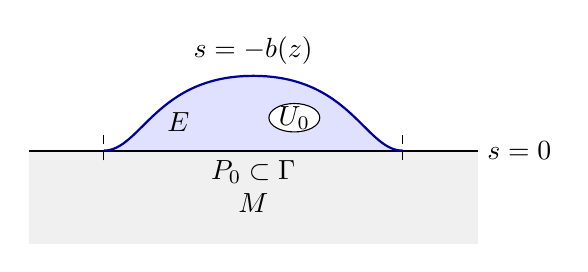
\begin{tikzpicture}[scale=0.95]
 \fill[gray!12] (-3,-1.25) rectangle (3,0);
 \fill[blue!12] (-2,0) .. controls (-1.5,0) and (-1.3,1.0) .. (0,1.0)
                 .. controls (1.3,1.0) and (1.5,0) .. (2,0) -- cycle;
 \draw[thick] (-3,0)--(3,0);
 \draw[thick,blue!60!black] (-2,0)
                 .. controls (-1.5,0) and (-1.3,1.0) .. (0,1.0)
                 .. controls (1.3,1.0) and (1.5,0) .. (2,0);
 \draw[dashed] (-2,-0.13)--(-2,0.23);
 \draw[dashed] (2,-0.13)--(2,0.23);
 \node at (0,-0.7) {$M$};
 \node at (-1,0.38) {$E$};
 \draw[fill=white] (0.55,0.44) ellipse (0.34 and 0.19);
 \node at (0.55,0.44) {$U_0$};
 \node[above] at (0,1.02) {$s=-b(z)$};
 \node[below] at (0,0) {$P_0\subset\Gamma$};
 \node[right] at (3,0) {$s=0$};
\end{tikzpicture}
\caption{A local schematic cross-section of the common exterior cap.
The boundary moves only over a compact subset of the measured patch.
The oval is a nonempty open source set $U_0$ with closure inside $E$.
The proof uses the smooth graph $s=-b(z)$, also at points where $b=0$.}
\label{data:cap-figure}
\end{figure}

\subsection{Harmonic functions from sources in the cap}

For $f\in C_c^\infty(U_0)$, let $u_f^j$ solve $L_{g_j}u_f^j=f$ on
$M_j^e$ with zero Dirichlet data, as in \eqref{data:green-normalization}.
Define the linear functional $I_j(p)$ by
\begin{equation}\label{data:evaluations}
 I_j(p)(f)=u_f^j(p).
\end{equation}
Thus $I_1(p)=I_2(q)$ means
$u_f^1(p)=u_f^2(q)$ for every $f\in C_c^\infty(U_0)$.
Proposition~\ref{data:cap} gives $I_1(p)=I_2(p)$ for $p\in E$.
The equation $L_{g_j}u_f^j=f$ makes $u_f^j$ harmonic on
$(M_j^e)^\circ\setminus\overline{U_0}$.

The use of evaluations to identify points follows
\citet[Definitions~2.1 and~6.1]{LLS20}. Their Runge approximation
and point separation for solutions with interior sources are in
\citep[Propositions~A.6 and~A.7]{LLS20}. The proof of
Lemma~\ref{data:jet-family}(ii) represents functionals of second
jets as distributions supported at one point, as in
\citep[Chapter~III, Section~3, proof of Theorem~6]{Malgrange1956}.

\begin{lemma}[Point separation and prescribed harmonic second jets]\label{data:jet-family}
Let $(N,g)$ be a compact connected smooth manifold with nonempty
boundary and dimension $n\ge2$. Let $U\Subset N^\circ$ be
nonempty and open, and let $R=L_{g,D}^{-1}$ be the inverse for
zero Dirichlet data.
\begin{enumerate}[label=\textup{(\roman*)}]
 \item The functionals $I(p):f\mapsto Rf(p)$,
       $f\in C_c^\infty(U)$, separate distinct interior points.
       They are nonzero in the interior and zero on the boundary.
       For each fixed $f$, $p\mapsto Rf(p)$ is continuous on $N$.
 \item If $p\in N^\circ\setminus\overline U$, every second jet at
       $p$ satisfying $L_g u(p)=0$ is the second jet of $Rf$ for
       some $f\in C_c^\infty(U)$. In particular, one can choose $n$
       source solutions whose differentials at $p$ are linearly
       independent, and hence form harmonic coordinates near $p$.
       In these coordinates the matrices
       $(\partial_a\partial_b Rf(p))$ span
       $\{H\in\operatorname{Sym}^2(\mathbb R^n):g^{ab}(p)H_{ab}=0\}$.
\end{enumerate}
\end{lemma}

\begin{proof}
For $f\in C_c^\infty(U)$, Dirichlet regularity gives
$Rf\in C^\infty(N)$ and the trace is zero. If $f\ge0$ and
$f\not\equiv0$, the strong maximum principle for $-\Delta_g Rf=f$
gives $Rf>0$ on $N^\circ$, so the interior functionals are nonzero.

For part (ii), let $T$ be a functional on second jets at $p$ that
annihilates the jets of all $Rf$ with $f\in C_c^\infty(U)$. Regard
$T$ as a distribution of order at most two supported at $p$.
Define $w=RT$ by $\langle w,f\rangle=\langle T,Rf\rangle$ for
$f\in C_c^\infty(N^\circ)$, with the pairing taken relative to
$\dd V_g$. Then $L_gw=T$ since $RL_gf=f$ for these test functions,
and $w=0$ on $U$ by the choice of $T$. Elliptic regularity gives
$\Delta_gw=0$ smoothly on $N^\circ\setminus\{p\}$. This set is
connected since paths can be diverted around $p$ in a coordinate
ball when $n\ge2$. Interior unique continuation
\citep[Theorem~8]{KochTataru2005} gives $\supp w\subset\{p\}$.

A distribution supported at one point is a finite sum
\[
 w=\sum_{|\alpha|\le k}c_\alpha\partial^\alpha\delta_p.
\]
If $w\ne0$, take $k$ to be the largest $|\alpha|$ with
$c_\alpha\ne0$. The terms of order $k+2$ in $L_gw$ have coefficients
given by the product of $\sum_{|\alpha|=k}c_\alpha\xi^\alpha$ and
$-g^{ab}(p)\xi_a\xi_b$. Both factors are nonzero polynomials, so
$L_gw$ has order $k+2$. Since $L_gw=T$ has order at most two,
$w=c\delta_p$ and $T(u)=cL_gu(p)$. Conversely, $L_gRf(p)=f(p)=0$
since $p\notin\overline U$. The annihilator of the jets of $Rf$
is therefore spanned by $u\mapsto L_gu(p)$, so finite-dimensional
duality gives the full subspace of jets satisfying $L_gu(p)=0$.

For part (i), suppose $I(p)=I(q)$ for distinct interior points and
put $T=\delta_p-\delta_q$. The definition of $RT$ gives
\[
 \langle RT,f\rangle=Rf(p)-Rf(q)=0,
 \qquad f\in C_c^\infty(U).
\]
Since $L_gRT=T$, $RT$ is harmonic on the connected set
$N^\circ\setminus\{p,q\}$ and vanishes on $U\setminus\{p,q\}$.
Interior unique continuation \citep[Theorem~8]{KochTataru2005}
gives $\supp RT\subset\{p,q\}$. Near $p$, $L_gRT=\delta_p$, so
$RT$ is nonzero there. Multiplication of its highest-order
coefficient polynomial by $-g^{ab}(p)\xi_a\xi_b$ makes the order of
$L_gRT$ at least two near $p$, contradicting $L_gRT=\delta_p$ there.
Thus $I(p)\ne I(q)$.

The condition $L_g u(p)=0$ allows arbitrary $\dd u(p)$ by
choosing the second derivatives to satisfy the equation. Part (ii)
thus gives $n$ solutions $Rf$ whose differentials at $p$ form a
basis of $T_p^*N$. They define harmonic coordinates near $p$.
Since the coordinate functions satisfy $\Delta_g x^a=0$, in these
coordinates $\Delta_g=g^{ab}\partial_a\partial_b$. Applying part (ii)
with $\dd u(p)=0$ gives a family of coordinate Hessians spanning
$\{H:g^{ab}(p)H_{ab}=0\}$. A basis chosen at $p$ remains linearly
independent in a sufficiently small neighborhood by continuity.
\end{proof}

\begin{remark}\label{data:local-pairs}
The two functions $u_f^j$ in \eqref{data:evaluations} have the
same source $f\in C_c^\infty(U_0)$. In Proposition~\ref{global:frontier},
Lemma~\ref{data:jet-family}(ii) supplies the harmonic coordinates
and pairs satisfying the Hessian condition of Theorem~\ref{local:extension}
outside $\overline{U_0}$. The order \eqref{local:parameter-order}
fixes these functions before the dilation \eqref{cross:dilation}
and the limit $\delta\downarrow0$ in \eqref{balls:radius}.
The constant function $1$ is used separately in \eqref{balls:reproduction}.
\end{remark}
\section{Local continuation for two elliptic equations}
\label{cross:section}

\subsection{The local metric extension theorem}

Proposition~\ref{data:cap} gives $g_1=g_2$ on the identified cap
$E$. Proposition~\ref{global:frontier} enlarges this isometry by using
source-generated harmonic coordinates to identify neighborhoods of
two interior points. The local statement needed there is that
equality of the coordinate metrics on one side of a smooth
hypersurface, together with the Green-kernel and harmonic-function
equalities stated below, extends across the hypersurface.

\begin{theorem}[Local metric extension]\label{local:extension}
Let $n\geq3$.  Let $(N_1,g_1)$ and $(N_2,g_2)$ be smooth compact
connected Riemannian manifolds with nonempty smooth boundary, with
Dirichlet Green functions $G_1,G_2$.  Identify two interior harmonic
coordinate neighborhoods with one neighborhood $\Omega\subset
\mathbb R^n$ of $0$.  Suppose an open $W\subset\Omega$ contains, near
$0$, one side of a smooth hypersurface through $0$, and suppose
\[
 g_1=g_2\text{ on }W,\qquad
 G_1(x,y)=G_2(x,y)\quad(x,y\in W,\ x\ne y).
\]
Suppose there are finitely many smooth pairs $(u_1^a,u_2^a)$ on
$\Omega$ such that $\Delta_{g_j}u_j^a=0$ and $u_1^a=u_2^a$ on $W$,
and such that the coordinate Hessian matrices
$(\partial_i\partial_j u_1^a(0))$, formed from ordinary second
partial derivatives in the common harmonic coordinates, span
\[
 \{H\in\operatorname{Sym}^2(\mathbb R^n):g_1^{ij}(0)H_{ij}=0\}.
\]
Here $H=(H_{ij})$ denotes a real symmetric matrix.
Then the two coordinate metrics agree on a neighborhood of $0$.
\end{theorem}

The proof of Theorem~\ref{local:extension} is completed in
Section~\ref{sec:bootstrap}. Proposition~\ref{cross:initial} first
continues the mixed Green data \eqref{cross:mixed-data} to prescribed
compact sets at positive distance from $x=y$, after a sufficiently
small spatial dilation. Proposition~\ref{balls:continuation} then
continues the kernel to the spheres of radius $r_\delta$ in
\eqref{balls:radius}, under the condition
\eqref{balls:bootstrap-condition}. Its metric inequality is
$H_8\le\eps r_\delta$, where
$H_8=\sum_{|\alpha|\le8}|\partial^\alpha h|$ and
$h=Q-\gamma^{-1}$ is defined in \eqref{balls:normalization}.
The flux functional $T_y$ in \eqref{balls:flux} satisfies the
reproduction identities \eqref{balls:reproduction} for the dilated
functions $u_j^a(\lambda\cdot)$, constants, and coordinates.

Lemma~\ref{local:density} bounds the density $\psi$ in
\eqref{balls:density-representation} uniformly as $\delta$ tends to
zero. Together with \eqref{balls:reproduction}, this gives
\eqref{local:moment-bound} for
$\lambda^{-2}\bigl(u_2^a(\lambda y)-u_1^a(\lambda y)\bigr)$, the
difference of the functions $\lambda^{-2}v_j^a(\lambda\cdot)$
from \eqref{local:renormalized-pairs}.
The Hessian system \eqref{local:metric-system} and
Lemma~\ref{local:interpolation} yield the strict improvement
\eqref{local:superlinear}. The argument in
Section~\ref{sec:bootstrap} can then send $\delta$ to zero while
holding the spatial dilation fixed, obtaining $h=0$ near $0$.
Equation~\eqref{balls:normalization} makes the metrics conformal, and
their common harmonic coordinates and equality on $W$ make them equal.
The continuation results in this section are used at positive distance
from the diagonal; their estimates are not required to be uniform as
that distance tends to zero.

\subsection{Extension from two intersecting product domains}

We begin with a statement for general scalar elliptic operators. Let
$L_i$ be a smooth scalar second-order elliptic operator in a coordinate
domain, with real positive definite principal matrix $g_i^{-1}$.
Lower-order terms are allowed. We consider a function $F(x,y)$
satisfying
\[
 L_1^xF=0,\qquad L_2^yF=0.
\]
It also satisfies $(L_1^x+L_2^y)F=0$, and this sum is elliptic
on the product domain. Unique continuation therefore applies.
We construct extensions explicitly and use unique continuation to
prove agreement of extensions already constructed.

The data will be solutions on $D_1\times S_2$ and
$S_1\times D_2$ which agree on $S_1\times S_2$, where
$S_i\Subset D_i$. An orthonormal basis of the $L_1$-solution space
on $D_1$ that is also orthogonal after restriction to $S_1$ will
construct the extension. Such common-basis methods for separately
harmonic extension have a classical antecedent in
\citet{Zeriahi1982}; singular systems also enter quantitative Runge
approximation \cite{RulandSalo2019}. The proof below gives the
variable-coefficient construction and states which bounds control
its constants.

\begin{lemma}[Extension from a cross]\label{cross:series}
Let $D_i$ be bounded connected coordinate domains and
$S_i\Subset D_i$ nonempty open sets. Suppose $F$ satisfies
$L_1^xF=L_2^yF=0$ on
\[
 (D_1\times S_2)\cup(S_1\times D_2),
\]
with the two definitions agreeing on $S_1\times S_2$, and suppose
$\|F\|_{L^2(D_1\times S_2)}+
\|F\|_{L^2(S_1\times D_2)}\le M$.
Let $O_i\Subset D_i$ be open sets such that every $L_i$-solution $w$
on $D_i$ satisfies
\begin{equation}\label{cross:interpolation-input}
 \|w\|_{L^2(O_i)}
 \le C\|w\|_{L^2(S_i)}^{\gamma_i}
          \|w\|_{L^2(D_i)}^{1-\gamma_i},
 \qquad 0<\gamma_i<1,\qquad \gamma_1+\gamma_2>1.
\end{equation}
Then $F$ extends to a solution of $L_1^xF=L_2^yF=0$ on
$O_1\times O_2$, agreeing with the original values on
$(O_1\times O_2)\cap(D_1\times S_2)$ and
$(O_1\times O_2)\cap(S_1\times D_2)$. For every compact
$K\Subset O_1\times O_2$, the extension satisfies
$\|F\|_{C^m(K)}\le C_{m,K}M$.
These constants are uniform when the distances in the compact
containments $S_i\Subset D_i$, $O_i\Subset D_i$, and
$K\Subset O_1\times O_2$, the ellipticity constants, the required
coefficient norms, and the constant $C$ in
\eqref{cross:interpolation-input} are controlled uniformly, and
$\gamma_1+\gamma_2-1$ has a uniform positive lower bound.
Each output order $m$ requires only finitely many coefficient norms.
\end{lemma}

\begin{proof}
Let $\mathcal H_1(D_1)$ be the closed subspace of $L^2(D_1)$ consisting
of distributional $L_1$-solutions.  Restriction
$R:\mathcal H_1(D_1)\to L^2(S_1)$ is compact by interior elliptic
estimates and injective by unique continuation.  The spectral theorem
for $R^*R$ gives an orthonormal basis $(w_j)$ of
$\mathcal H_1(D_1)$ such that
\begin{equation}\label{cross:singular-values}
 (w_i,w_j)_{L^2(S_1)}=\mu_j^2\delta_{ij},
 \qquad 0<\mu_j\le1.
\end{equation}
For every $N$,
\begin{equation}\label{cross:singular-decay}
 \mu_j\le C_N(1+j)^{-N}.
\end{equation}
Indeed, multiply a solution by a cutoff equal to one near
$\overline{S_1}$ and compactly supported in $D_1$. Interior elliptic
estimates bound its $H^k$ norm by its $L^2(D_1)$ norm. Fourier
truncation in a containing cube gives a rank $O(A^n)$ approximation
with operator error $O(A^{-k})$. The minimax characterization of
singular values yields $\mu_j\le C_kj^{-k/n}$.
The constants depend on the cutoff, the cube, the distance of the
cutoff support from $\partial D_1$, and the ellipticity and coefficient
bounds in the interior estimate.

For $y\in S_2$ expand $F(\cdot,y)$ on $D_1$:
\[
 F(x,y)=\sum_j w_j(x)b_j(y),\qquad
 \|b_j\|_{L^2(S_2)}\le M.
\]
Equation~\eqref{cross:singular-values} continues these coefficients to
$D_2$ by the formula
\begin{equation}\label{cross:coefficient-extension}
 b_j(y)=\mu_j^{-2}\int_{S_1}F(x,y)\overline{w_j(x)}\,\dd x,
 \qquad \|b_j\|_{L^2(D_2)}\le M\mu_j^{-1}.
\end{equation}
The function $b_j$ defined by
\eqref{cross:coefficient-extension} solves $L_2b_j=0$ on $D_2$ and
equals the coefficient of $w_j$ in the expansion of $F(\cdot,y)$
when $y\in S_2$. Applying \eqref{cross:interpolation-input}
to $w_j$ and to $b_j$ gives
\[
 \|w_j\|_{L^2(O_1)}\le C\mu_j^{\gamma_1},\qquad
 \|b_j\|_{L^2(O_2)}\le CM\mu_j^{\gamma_2-1}.
\]
Consequently the series converges absolutely in $L^2(O_1\times O_2)$:
its summands are bounded by $CM\mu_j^{\gamma_1+\gamma_2-1}$.
Choose $N$ in \eqref{cross:singular-decay} so that
$N(\gamma_1+\gamma_2-1)>1$.  The limit solves both equations
in distributions.  Interior estimates for their elliptic sum give
the asserted smoothness and bounds on smaller sets.

To prove agreement with the given values on $S_1\times O_2$,
let $z\in L^2(S_1)$ be orthogonal to the closure of
$R\mathcal H_1(D_1)$. The function
\[
 y\longmapsto\int_{S_1}F(x,y)\overline{z(x)}\,\dd x
\]
is annihilated by $L_2$ on $D_2$ and vanishes on $S_2$, hence vanishes
on the connected domain $D_2$. Consequently
$F(\cdot,y)|_{S_1}$ belongs to
$\overline{R\mathcal H_1(D_1)}$ for every $y\in D_2$.
Its expansion in the orthonormal basis $w_j/\mu_j$ has coefficients
$\mu_jb_j(y)$ by \eqref{cross:coefficient-extension}. Thus
$\sum_j w_j(x)b_j(y)=F(x,y)$ on $S_1\times O_2$.
The $L^2(S_1\times O_2)$ norm of the $j$th summand is bounded by
$CM\mu_j^{\gamma_2}$; on $O_1\times S_2$ it is bounded by
$CM\mu_j^{\gamma_1}$. Equation~\eqref{cross:singular-decay} gives
convergence on both sets, proving agreement with both original
restrictions. All bounds use only upper estimates for $\mu_j$,
so the constants require neither a continuous choice of the basis
$(w_j)$ nor positive lower bounds for its singular values.
\end{proof}

Figure~\ref{cross:figure} summarizes the sets and the two estimates in
Lemma~\ref{cross:series}.
\begin{figure}[htbp]
 \centering
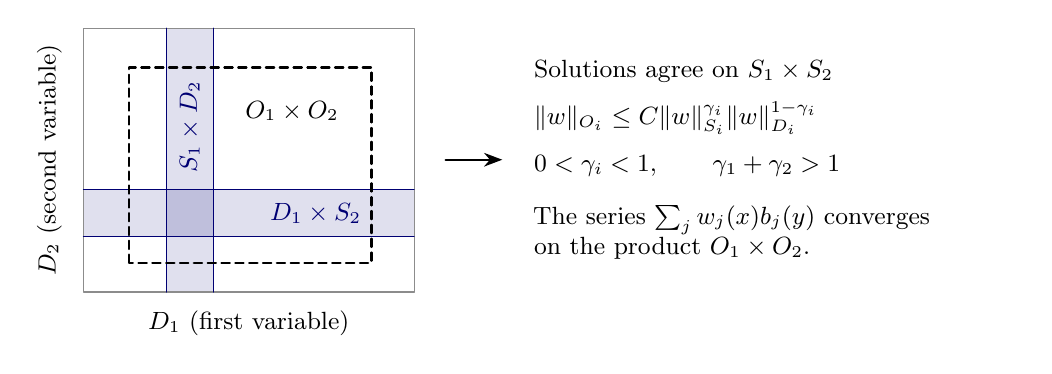
\begin{tikzpicture}[x=1cm,y=1cm,font=\small,>=Stealth,
  line cap=round,line join=round]
  \colorlet{crossink}{blue!45!black}
  \fill[crossink!12] (0,0.70) rectangle (4.2,1.30);
  \fill[crossink!12] (1.05,0) rectangle (1.65,3.35);
  \fill[crossink!25] (1.05,0.70) rectangle (1.65,1.30);
  \draw[black!45] (0,0) rectangle (4.2,3.35);
  \draw[crossink,thin] (0,0.70)--(4.2,0.70)
    (0,1.30)--(4.2,1.30) (1.05,0)--(1.05,3.35)
    (1.65,0)--(1.65,3.35);
  \draw[densely dashed,thick] (0.58,0.37) rectangle (3.66,2.85);
  \node[fill=white,inner sep=3pt] at (2.65,2.30) {$O_1\times O_2$};
  \node[text=crossink] at (2.95,1.00) {$D_1\times S_2$};
  \node[text=crossink,rotate=90] at (1.35,2.10) {$S_1\times D_2$};
  \node[anchor=north] at (2.10,-0.12) {$D_1$ (first variable)};
  \node[rotate=90,anchor=south] at (-0.15,1.68) {$D_2$ (second variable)};
  \draw[->,thick] (4.60,1.68)--(5.32,1.68);
  \node[anchor=west,align=left,text width=6.10cm] at (5.60,1.68) {
    Solutions agree on $S_1\times S_2$\\[6pt]
    $\displaystyle
       \|w\|_{O_i}\leq C\|w\|_{S_i}^{\gamma_i}
                              \|w\|_{D_i}^{1-\gamma_i}$\\[6pt]
    $\displaystyle 0<\gamma_i<1,\qquad \gamma_1+\gamma_2>1$\\[8pt]
    The series $\sum_jw_j(x)b_j(y)$ converges\\
    on the product $O_1\times O_2$.
  };
\end{tikzpicture}
 \caption{Solutions of $L_1^xF=L_2^yF=0$ are given on the two
 shaded product sets and agree on $S_1\times S_2$.
 The interpolation estimates \eqref{cross:interpolation-input},
 with $\gamma_1+\gamma_2>1$, make $\sum_jw_j(x)b_j(y)$ converge
 on $O_1\times O_2$.
 The drawing is schematic: each factor is a multidimensional domain,
 and containment of $S_i$ in $O_i$ is not required.}
 \label{cross:figure}
\end{figure}

\subsection{A geometric criterion for local extension}

We next construct the interpolation estimates
\eqref{cross:interpolation-input}. For a metric $g$, consider a smooth
real function $\theta$ with $\dd\theta\ne0$ and satisfying
\begin{equation}\label{cross:strict-weight}
 \operatorname{Hess}_g\theta(e,e)
  +\operatorname{Hess}_g\theta(v,v)>0
 \quad\text{for all }v\perp e,\ |v|_g=1,
 \qquad e=\frac{\nabla^g\theta}{|\nabla^g\theta|_g}.
\end{equation}
The strict scalar Carleman estimate gives, after shrinking the
coordinate neighborhood,
\begin{equation}\label{cross:carleman}
 \tau^3\|e^{\tau\theta}w\|_{L^2}^2
 +\tau\|\nabla(e^{\tau\theta}w)\|_{L^2}^2
 \le C\|e^{\tau\theta}Lw\|_{L^2}^2,
 \qquad \tau\ge\tau_0,
\end{equation}
for compactly supported $w$.
Estimate~\eqref{cross:carleman}, under the strict Hessian condition
\eqref{cross:strict-weight}, is a classical elliptic Carleman estimate;
see \citet[Chapter~XXVIII]{HormanderIV2009} and
\citet[Definition~8.3 and Theorem~9(a)]{KochTataru2005}.
Here the hypotheses can also be checked directly.  For $L=-\Delta_g$,
write $v=e^{\tau\theta}w$ and
\[
 e^{\tau\theta}Le^{-\tau\theta}=A_\tau+B_\tau,\qquad
 A_\tau=-\Delta_g-\tau^2|\dd\theta|_g^2,\quad
 B_\tau=\tau(2\nabla^g\theta\cdot\nabla+\Delta_g\theta).
\]
Here $A_\tau$ is self-adjoint and $B_\tau$ is skew-adjoint for
metric volume.  Integration by parts gives
\begin{align*}
 \|(A_\tau+B_\tau)v\|^2
 &=\|A_\tau v\|^2+\|B_\tau v\|^2
       +([A_\tau,B_\tau]v,v),\\
 ([A_\tau,B_\tau]v,v)
 &=4\tau\int\operatorname{Hess}_g\theta(\nabla v,\nabla\overline v)
   +4\tau^3\int\operatorname{Hess}_g\theta
                 (\nabla\theta,\nabla\theta)|v|^2
   -\tau\int(\Delta_g^2\theta)|v|^2.
\end{align*}
Condition~\eqref{cross:strict-weight} permits a real constant $m$
such that, at the point under consideration,
\[
 -\min_{v\perp e,\ |v|_g=1}\operatorname{Hess}_g\theta(v,v)
 <m<\operatorname{Hess}_g\theta(e,e).
\]
After shrinking the neighborhood, both inequalities hold with a
uniform positive margin. Adding $4m\tau(A_\tau v,v)$ to
$([A_\tau,B_\tau]v,v)$ makes its gradient coefficient
$4\tau(\operatorname{Hess}_g\theta+mg)$ and its leading coefficient
of $|v|^2$ equal to
\[
 4\tau^3|\dd\theta|_g^2
       \big(\operatorname{Hess}_g\theta(e,e)-m\big)>c\tau^3.
\]
The restriction of $\operatorname{Hess}_g\theta+mg$ to
$e^\perp$ is positive definite. After absorbing the mixed terms into
this positive tangential part, its remaining contribution is bounded
below by $-C\tau\|\nabla_e v\|^2$. Moreover,
\[
 \|\nabla_e v\|^2
 \le C\tau^{-2}\|B_\tau v\|^2+C\|v\|^2.
\]
Finally
$|4m\tau(A_\tau v,v)|\le\tfrac12\|A_\tau v\|^2+
C\tau^2\|v\|^2$.
For sufficiently large $\tau$, the term $\|B_\tau v\|^2$ absorbs
$C\tau\|\nabla_e v\|^2$ using the preceding bound, while
$c\tau^3\|v\|^2$ absorbs the resulting $C\tau\|v\|^2$ and
$C\tau^2\|v\|^2$ terms. This proves \eqref{cross:carleman}.
Smooth first- and zero-order terms in $L$ contribute at most
$C(\|\nabla v\|^2+\tau^2\|v\|^2)$ to the squared norm and are
absorbed by the left side of \eqref{cross:carleman} for larger $\tau$.
The constants are uniform when $|\dd\theta|_g$ and the positive
margin in \eqref{cross:strict-weight} are bounded below, and the
required coefficient and weight derivatives are bounded above.

The existence criterion is a condition on a hypersurface in the
product.  Hessians in the following statement use the product
connection of $g_1$ and $g_2$.

\begin{proposition}[Product extension criterion]\label{cross:criterion}
Let $\rho$ be smooth near $z_0=(x_0,y_0)$, with $\rho(z_0)=0$ and
$\dd_x\rho,\dd_y\rho\ne0$.  Put
\[
 a_i=\frac{\nabla_i\rho}{|\nabla_i\rho|^2},\qquad H=\operatorname{Hess}\rho.
\]
Suppose that at $z_0$
\begin{equation}\label{cross:hessian-test}
 H((a_1,-a_2),(a_1,-a_2))
 +H((v_1,v_2),(v_1,v_2))>0
 \quad
 \left(v_i\perp a_i,\ |v_i|=|a_i|\right).
\end{equation}
Every function $F$ satisfying $L_1^xF=L_2^yF=0$ on
$\{\rho>0\}$ near $z_0$ extends to a solution of the same two
equations on a neighborhood of $z_0$, with equality to the prescribed
$F$ on its intersection with $\{\rho>0\}$ after the neighborhood
is shrunk. The construction uses the values of $F$ on only two
compact product sets contained in $\{\rho>\epsilon\}$ for some
$\epsilon>0$.
The neighborhoods and estimates on smaller neighborhoods are uniform
under small smooth perturbations preserving the strict hypotheses,
provided the data on those compact sets are bounded.
\end{proposition}

\begin{proof}
We first use \eqref{cross:hessian-test} to construct functions
$\theta_i$ satisfying \eqref{cross:strict-weight} in the two
factors and the quadratic inequality \eqref{cross:quadratic-gap}.
That inequality places $\overline{D_1\times S_2}$ and
$\overline{S_1\times D_2}$ in $\{\rho>0\}$. Applying
\eqref{cross:carleman} with these functions gives
\eqref{cross:interpolation-input} with the exponents
\eqref{cross:exponent}, both greater than $1/2$, so that
Lemma~\ref{cross:series} applies.

\paragraph{Splitting the weight between the factors.}
We seek symmetric forms $P_i$ satisfying
\[
 P_i(a_i,a_i)+P_i(v_i,v_i)>0,
 \qquad H+K\,\dd\rho^{\otimes2}>P_1\oplus P_2
\]
for some $K>0$, for every $v_i\perp a_i$ with
$|v_i|=|a_i|$. Dividing the first inequality by $|a_i|^2$ gives
\eqref{cross:strict-weight} for a function with gradient
$\nabla_i\rho$ and Hessian $P_i$. The second inequality gives
\eqref{cross:quadratic-gap}. Convex separation reduces the existence
of these $P_i$ to testing positive semidefinite symmetric tensors
$D$ whose diagonal blocks have the form
\[
 d_i a_i^{\otimes2}+S_i,\qquad
 d_i\ge0,\quad S_i\ge0\text{ on }a_i^\perp,
 \quad \tr S_i=d_i|a_i|^2.
\]
Indeed, consider the open convex cone of sums of a positive
definite form and a block form $P_1\oplus P_2$ satisfying
$P_i(a_i,a_i)+P_i(v_i,v_i)>0$ for all
$v_i\perp a_i$, $|v_i|=|a_i|$. Its dual consists of positive
semidefinite tensors $D$ with the displayed diagonal blocks, because
the dual cone in the $i$th factor is generated by
$a_i^{\otimes2}+v_i^{\otimes2}$ with these constraints on $v_i$.
Normalize $\tr D=1$. By compactness, it suffices to prove
$H:D>0$ for these tensors when $D\,\dd\rho=0$; a sufficiently large
$K$ then makes $(H+K\,\dd\rho^{\otimes2}):D>0$ for every normalized
tensor in the dual cone.

Extend the partial covectors $\dd_1\rho$ and $\dd_2\rho$ by
zero on the other factor. The identity $D\,\dd\rho=0$ gives
\[
 D(\dd_1\rho,\dd_1\rho)
 =D(\dd_2\rho,\dd_2\rho)
 =-D(\dd_1\rho,\dd_2\rho).
\]
The prescribed diagonal blocks make each normal component orthogonal,
with respect to $D$, to the tangential covectors in its own factor.
The same identity $D\,\dd\rho=0$ makes it orthogonal to those in
the other factor as well. Since $\dd_i\rho(a_i)=1$, the equal
normal components of $D$ give $d_1=d_2=d>0$ and
\[
 D=d(a_1,-a_2)^{\otimes2}+D_\perp,
 \qquad \tr(D_\perp)_{ii}=d|a_i|^2.
\]
If $d=0$, positivity and the trace conditions force $D=0$,
contrary to $\tr D=1$. Among positive semidefinite $D_\perp$ with
the two stated traces, every extreme point has rank one: on an image
of rank $r\ge2$, the space of symmetric perturbations has dimension
$r(r+1)/2>2$, so a nonzero perturbation can preserve both traces,
and sufficiently small perturbations of both signs preserve positivity.
For a rank-one tensor,
$D_\perp=d(v_1,v_2)^{\otimes2}$ with
$v_i\perp a_i$ and $|v_i|=|a_i|$. Therefore
\[
 H:D=d\bigl[
 H((a_1,-a_2),(a_1,-a_2))
 +H((v_1,v_2),(v_1,v_2))\bigr]>0
\]
by \eqref{cross:hessian-test}. Convexity gives the same strict
positivity for all admissible $D_\perp$. Compactness of the tensors
with $\tr D=1$ then gives the required $K$.

Prescribe gradients $\dd_i\rho$ and Hessians $P_i$ for smooth functions
$\theta_i$ vanishing at the respective points.  In small coordinates
centered there, Taylor expansion gives
\begin{equation}\label{cross:quadratic-gap}
 \theta_1(x)+\theta_2(y)
 \le \widetilde\rho(x,y)-c(|x|^2+|y|^2),
 \qquad \widetilde\rho=\rho+K\rho^2/2,
\end{equation}
with $c>0$.  Each $\theta_i$ satisfies
\eqref{cross:strict-weight}.  The positive side of $\widetilde\rho$
is the positive side of $\rho$ in this neighborhood.

\paragraph{Placing the cross and obtaining interpolation.}
Use coordinates $(s_i,z_i)$ with $s_i=\theta_i$. Fix a small
$\kappa>0$ so that $\phi(s_i)=s_i-\kappa s_i^2$ still satisfies
\eqref{cross:strict-weight}. Choose successively a small lateral
radius $R$, a height $l\ll cR^2$, and $e\ll\kappa l^2$. Take
\[
 D_i=\{-l<s_i<l+4e,\ |z_i|<R\}.
\]
Use a cutoff equal to one on the inner lateral half and for
$-l+3e<s_i<l+2e$, supported in the cylinder and in
$-l+2e<s_i<l+3e$.
Let $S_i\Subset D_i$ include neighborhoods of its top and lateral
derivative supports, where respectively
\[
 s_i>l+e/2\quad\text{or}\quad |z_i|>R/3,
\]
and an inner top slice near $s_i=l+5e/4$.
The closed product sets $\overline{D_1\times S_2}$ and
$\overline{S_1\times D_2}$ are contained in $\{\rho>0\}$.
If the factor from $S_i$ lies in its top part, then $s_1+s_2>0$.
If it lies in its lateral part, then $s_1+s_2>-2l$, while
$c(|x|^2+|y|^2)>2l$ by the choice $l\ll cR^2$.
In either case \eqref{cross:quadratic-gap} gives
$\widetilde\rho>0$, hence $\rho>0$.
Making the sets slightly smaller if necessary gives a common
$\epsilon>0$ with $\rho>\epsilon$ on their closures.

For an $L_i$-solution normalized by $\|w\|_{L^2(D_i)}=1$, apply
\eqref{cross:carleman} to the chosen cutoff times $w$.
On the support of the lower cutoff derivative, interior estimates use
$\|w\|_{L^2(D_i)}$ and the weight is at most $\phi(-l+3e)$.
On the supports of the upper and lateral cutoff derivatives, they use
$\|w\|_{L^2(S_i)}$ and the weight is at most $\phi(l+3e)$.
On a smaller inner cylinder beginning at $s_i=-e$, the weight is at
least $\phi(-e)$. Balancing the two resulting exponential terms gives
\eqref{cross:interpolation-input} with
\begin{equation}\label{cross:exponent}
 \gamma_i=
 \frac{\phi(-e)-\phi(-l+3e)}{
       \phi(l+3e)-\phi(-l+3e)}>\frac12.
\end{equation}
At $e=0$, the quotient in \eqref{cross:exponent} equals
$1/2+\kappa l/2$. Values of the balancing parameter below $\tau_0$
are handled by increasing the constant in
\eqref{cross:interpolation-input}. The smaller cylinder $O_i$ in
that estimate can include a connected tube from the origin to the
top slice near $s_i=l+5e/4$.

\paragraph{Constructing and identifying the extension.}
Lemma~\ref{cross:series} gives a solution of $L_1^xF=L_2^yF=0$
on $O_1\times O_2$, which contains a neighborhood of $z_0$.
To verify agreement with the prescribed $F$ on $\{\rho>0\}$,
start at a sufficiently close point of this set and increase $s_2$
to the top slice near $s_2=l+5e/4$. Since $\partial_{s_2}\rho>0$
locally, this segment stays in $\{\rho>0\}\cap(O_1\times O_2)$.
At its upper end, the two solutions agree on the original product
set $D_1\times S_2$. Unique continuation for $L_1^x+L_2^y$ along
a neighborhood of the segment gives equality at the starting point.
The strict inequalities in \eqref{cross:strict-weight},
\eqref{cross:quadratic-gap}, and \eqref{cross:exponent} persist under
small smooth perturbations. Keeping the compact sets used for the
cutoffs and shrinking $O_i$ once therefore gives uniform estimates
from \eqref{cross:carleman}, Lemma~\ref{cross:series}, and interior
elliptic regularity.
\end{proof}

\subsection{Gluing along a compact family of surfaces}

Proposition~\ref{cross:criterion} extends a solution across one point
of $\{\rho=0\}$. The next lemma joins such local extensions along
a compact family of level surfaces. Unique continuation is applied
on each connected component of an overlap after equality has been
established on an open subset of that component.

\begin{lemma}[Propagation through a compact cylinder]
\label{cross:propagation}
Suppose a region in a product patch has smooth coordinates $(z,a)$
near $B\times[a_-,a_+]$, where $B$ is compact and may have boundary
or corners. Let $F$ satisfy $L_1^xF=L_2^yF=0$ on an open set
$\mathcal S$ containing neighborhoods of the top
$B\times\{a_+\}$ and the lateral boundary
$\partial B\times[a_-,a_+]$. Assume $\mathcal S$ is upward closed
in $a$ at fixed $z$. If every level $a=\mathrm{constant}$ satisfies
the hypotheses of Proposition~\ref{cross:criterion} outside
$\mathcal S$, with $\{\rho>0\}$ corresponding locally to larger
$a$, then $F$ extends to a solution of the same two equations on
a neighborhood of the cylinder, agreeing with its prescribed values
on $\mathcal S$.
For fixed coordinates, compact sets and strict reference inequalities,
the extension has uniform compact-subset bounds under small smooth
perturbations, in terms of bounds on finitely many compact subsets of
the initially given region.
\end{lemma}

\begin{proof}
Starting at $a_+$, let $a_*$ be the infimum of the levels $a$
for which an extension to a neighborhood of $B\times[a,a_+]$
has been obtained, agreeing with $F$ on $\mathcal S$. For the
uniform assertion, require the stated compact-subset bounds as well.
At each point of $B\times\{a_*\}$ outside $\mathcal S$,
Proposition~\ref{cross:criterion} constructs an extension from compact
sets with $a>a_*$. Cover $B\times\{a_*\}$ by finitely many of
these neighborhoods and neighborhoods contained in $\mathcal S$.
The compact sets used for the new extensions all have
$a\ge a_*+\eta$ for some common $\eta>0$, so they are contained
in a region already reached by the extension and have the required
bounds. On the neighborhoods contained in $\mathcal S$, use the
prescribed function $F$.

Shrink the constructed neighborhoods to boxes
$B_i\times(a_*-d_i,a_*+d_i)$ in the $(z,a)$ coordinates.
Every connected component of an overlap contains a vertical segment
to some height $a>a_*$. Both local extensions equal the previously
constructed function near that height. Unique continuation for
$L_1^x+L_2^y$ therefore makes them equal on the whole overlap
component. The same argument proves agreement with $F$ on
$\mathcal S$: upward closure keeps each vertical segment starting
in $\mathcal S$ inside $\mathcal S$ until it reaches $a>a_*$.
On the given neighborhoods of
$B\times\{a_+\}$ and $\partial B\times[a_-,a_+]$, use $F$.
The finite cover has $\min_i d_i>0$, so the joined extension reaches
below $a_*$ unless $a_*=a_-$; in that case it includes a neighborhood
of the bottom level. Thus it is defined near the whole cylinder.
The strict inequalities required by Proposition~\ref{cross:criterion}
remain valid under small smooth perturbations. Its Carleman estimate
\eqref{cross:carleman}, the series estimates of
Lemma~\ref{cross:series}, and interior elliptic estimates give the
claimed uniform bounds for this finite construction. Each new local
extension uses compact data with $a>a_*$, so no bound up to an
unreached limiting level is assumed.
\end{proof}

\subsection{Initialization at a fixed distance from the diagonal}

We apply Proposition~\ref{cross:criterion} to a mixed Green kernel.
Let $g_1,g_2$ be smooth
metrics in coordinate patches centered at $0$, obtained from interior
patches of compact Dirichlet manifolds.  Suppose they agree on an open
set $W$ containing the lower side of a smooth hypersurface through $0$.
After a linear coordinate change, assume
\[
 g_1(0)=g_2(0)=I,\qquad
 \{x_n<q(x')\}\subset W\text{ near }0,\qquad
 q(0)=0,\quad \dd q(0)=0,
\]
for a smooth function $q$.  No regularity of the rest of $\partial W$
is assumed.
Let $G_j$ be the Dirichlet Green kernels, normalized with metric volume,
and suppose $G_1=G_2$ on $W\times W$.
For a small dilation parameter $\lambda>0$, use the metric with
coefficients $g_j(\lambda z)$ in the rescaled coordinates $z$.
By change of variables in \eqref{data:green-normalization},
\begin{equation}\label{cross:dilation}
 W_\lambda=\lambda^{-1}W,\qquad
 -\Delta_{g_j(\lambda\cdot),x}
    \bigl(\lambda^{n-2}G_j(\lambda x,\lambda y)\bigr)
     =\delta_y^{g_j(\lambda\cdot)}(x).
\end{equation}
On each fixed bounded patch the metrics tend smoothly to the Euclidean
metric, and $W_\lambda$ contains every fixed compact subset of
$\{z_n<0\}$ for sufficiently small $\lambda$.
Initially define, off the diagonal,
\begin{equation}\label{cross:mixed-data}
 \mathcal G_\lambda(x,y)=\lambda^{n-2}
 \begin{cases}
 G_1(\lambda x,\lambda y),&y\in W_\lambda,\\
 G_2(\lambda x,\lambda y),&x\in W_\lambda.
 \end{cases}
\end{equation}
The definitions in \eqref{cross:mixed-data} agree where
$x,y\in W_\lambda$.  Away from $x=y$, they satisfy
$\Delta_{g_1(\lambda\cdot),x}\mathcal G_\lambda=0$ and
$\Delta_{g_2(\lambda\cdot),y}\mathcal G_\lambda=0$.

\begin{proposition}[Fixed-separation initialization]\label{cross:initial}
In this setting, let $n\ge3$ and fix $B>0$, $d>0$ and $\eta>0$.
For all sufficiently small $\lambda$, the data
\eqref{cross:mixed-data} extend to a solution of
$\Delta_{g_1(\lambda\cdot),x}\mathcal G_\lambda=0$ and
$\Delta_{g_2(\lambda\cdot),y}\mathcal G_\lambda=0$ on a
neighborhood of
\[
 \{(x,y):|x|,|y|\le B,\ |x-y|\ge d\}.
\]
Every fixed $C^m$ norm on a smaller neighborhood is bounded uniformly
in $\lambda$. The continuation equals $\lambda^{n-2}G_1(\lambda x,\lambda y)$
where $y_n<-\eta$ and $\lambda^{n-2}G_2(\lambda x,\lambda y)$ where
$x_n<-\eta$, on the corresponding overlaps. The smallness threshold
for $\lambda$ and the constants may depend on $B,d,\eta,m$.
\end{proposition}

\begin{proof}
We first extend across $x_n=0$ and $y_n=0$ at positive distance from
$x=y$.  We then continue through the surfaces
$|x-y|=r_a(y)$ defined in \eqref{cross:tubes} to reach
$|x|,|y|\le B$ and $|x-y|\ge d$.
All sets and positive lower bounds for $|x-y|$ in these constructions
are fixed before choosing $\lambda$.

\paragraph{Extension across the coordinate planes.}
In \eqref{cross:interpolation-input}, we will obtain a fixed exponent
$\gamma_2>0$ for the $y$ variable and choose the domains in the $x$
variable so that $\gamma_1$ is sufficiently close to one.
Then $\gamma_1+\gamma_2>1$, as required by
Lemma~\ref{cross:series}.

Fix $x_0$ with $(x_0)_n=0$ and $s>0$.
In the $y$ variable take
\[
 D_2=\{y:s/2<|y-x_0|<2s\}
\]
and let $S_2\Subset D_2$ be a ball centered at $x_0-se_n$ and
contained in $\{y_n<0\}$.
In the $x$ variable take
\[
 D_1=B(x_0-\tau_0se_n,3\tau_0s),\qquad
 S_1=B(x_0-\tau_0se_n,(1-\alpha)\tau_0s).
\]
Choose $\tau_0>0$ sufficiently small that the closures of $D_1$ and
$D_2$ are disjoint.  The number $\alpha>0$ will be chosen below;
$S_1$ is contained in $\{x_n<0\}$.

For the $y$ variable in \eqref{cross:interpolation-input}, take
$O_2\Subset D_2$ to be an open annulus containing
$\{y:4s/5\le|y-x_0|\le6s/5\}$. The exponent $\gamma_2>0$ is
independent of $\alpha$.
To prove this with constants that remain uniform under small metric
perturbations, use the weight $|z-z_*|^{-1}$ on a Euclidean annulus.
It satisfies \eqref{cross:strict-weight}: its radial Hessian value is
$2|z-z_*|^{-3}$ and each unit tangential Hessian value is
$-|z-z_*|^{-3}$.
Apply \eqref{cross:carleman} with radial cutoffs and optimize in $\tau$
to obtain an estimate of the form \eqref{cross:interpolation-input}
for three concentric balls.
A finite chain of overlapping balls, with their enlarged balls inside
$D_2$, connects $S_2$ to each ball in a finite cover of $\overline{O_2}$,
since $D_2$ is connected. Iterating \eqref{cross:interpolation-input}
along these chains gives $\gamma_2>0$. The cutoff supports stay a fixed
distance from the boundaries of the larger balls, and
\eqref{cross:strict-weight} persists under sufficiently small
perturbations of the Euclidean metric.

For the $x$ variable, apply \eqref{cross:carleman} with radial cutoffs centered
at $x_0-\tau_0se_n$.  Keep the outer cutoff a fixed distance beyond
radius $\tau_0s$, and put the inner cutoff just inside radius
$(1-\alpha)\tau_0s$.  Take $O_1=B(x_0-\tau_0se_n,(\tau_0+c)s)$
with $c>0$ small. It contains $S_1$ and
$B(x_0,cs)$.
As $\alpha,c\downarrow0$, the weight values at the boundary of $O_1$
and on the inner cutoff approach one another, so $\gamma_1$ in
\eqref{cross:interpolation-input} approaches one. Choose $\alpha,c$ so that
$\gamma_1+\gamma_2>1$.
Lemma~\ref{cross:series} extends $\mathcal G_\lambda$ to
$O_1\times O_2$. Since $\dist(D_1,D_2)>0$, the local bound
$G_j(x,y)=O(|x-y|^{2-n})$ gives a uniform bound for
$\lambda^{n-2}G_j(\lambda x,\lambda y)$ on $D_1\times D_2$.
Interior elliptic estimates for \eqref{cross:dilation} give
uniform derivative bounds on its compact subsets.

Lemma~\ref{cross:series} gives
$\mathcal G_\lambda(x,y)=\lambda^{n-2}G_1(\lambda x,\lambda y)$ on
$O_1\times(S_2\cap O_2)$ and
$\mathcal G_\lambda(x,y)=\lambda^{n-2}G_2(\lambda x,\lambda y)$ on
$S_1\times O_2$. For small $\lambda$, $S_1,S_2\subset W_\lambda$
by \eqref{cross:dilation}. For fixed $x\in O_1\cap W_\lambda$,
$\mathcal G_\lambda(x,y)-\lambda^{n-2}G_2(\lambda x,\lambda y)$ is
annihilated by $\Delta_{g_2(\lambda\cdot),y}$ on $O_2$ and vanishes on
$S_2\cap O_2$ by \eqref{cross:mixed-data}. Unique continuation on
$O_2$ gives $\mathcal G_\lambda(x,y)=\lambda^{n-2}G_2(\lambda x,\lambda y)$
there. For fixed $y\in O_2\cap W_\lambda$, the same argument uses
$\Delta_{g_1(\lambda\cdot),x}$ on $O_1$ and equality on $S_1$ to give
$\mathcal G_\lambda(x,y)=\lambda^{n-2}G_1(\lambda x,\lambda y)$ on $O_1$.

Use smaller balls about $x_0$ and narrower annuli for the cover,
and compare the extensions on the original product domains.
In each product, $s$ is comparable to $|x-y|$.
On a fixed compact set disjoint from $x=y$, choose
$0<\eta_0\le\eta$ smaller than the distances from the smaller balls
and annuli to the boundaries of the larger ones. For sufficiently
small $\lambda$, the parts of $\{z_n<-\eta_0\}$ used here are contained
in $W_\lambda$ by \eqref{cross:dilation}.

If both balls are in the $x$ variable, move $x$ inside both larger
balls to $x_n<-\eta_0$, with $y$ fixed. Both extensions equal
$\lambda^{n-2}G_2(\lambda x,\lambda y)$ there, since $x\in W_\lambda$.
If both balls are in the $y$ variable, move $y$ inside both larger
balls to $y_n<-\eta_0$ and use $\lambda^{n-2}G_1(\lambda x,\lambda y)$.
If the balls are in different variables, translate
both $x$ and $y$ in the direction $-e_n$ by
$\max(x_n,y_n,0)+2\eta_0$. Choose the smaller balls sufficiently small
relative to the larger factors that this path stays in both original
products. At its endpoint $x_n,y_n<-\eta_0$, so both extensions agree
by \eqref{cross:mixed-data} and $G_1(\lambda x,\lambda y)=G_2(\lambda x,\lambda y)$
for $x,y\in W_\lambda$ with $x\ne y$.
The difference of the extensions is annihilated by
$\Delta_{g_1(\lambda\cdot),x}+\Delta_{g_2(\lambda\cdot),y}$ on a
connected neighborhood of each comparison path in the overlap.
It vanishes near the endpoint, so unique continuation gives
agreement at $(x,y)$.

The extensions therefore define one $\mathcal G_\lambda$ on the region
\begin{equation}\label{cross:coarse-region}
 \min(x_n,y_n)<c_0|x-y|,
\end{equation}
for sufficiently small $c_0>0$. On each fixed compact set in this region
disjoint from $x=y$, the $C^m$ bounds from Lemma~\ref{cross:series}
are uniform in $\lambda$.
For pairs satisfying \eqref{cross:coarse-region} and $0\le x_n\le y_n$, take
$x_0=(x',0)$ and $s=|y-x_0|$.
Then $x$ lies in the smaller ball and $y$ in the narrower annulus.
Treat $0\le y_n\le x_n$ by interchanging the variables.
For pairs with $x_n<0$ or $y_n<0$, use the same product neighborhoods
near $x_n=0$ or $y_n=0$, and use \eqref{cross:mixed-data} where
$x_n<-\eta_0$ or $y_n<-\eta_0$.

\paragraph{Continuation through decreasing radii.}
To extend $\mathcal G_\lambda$ from \eqref{cross:coarse-region}
to the pairs in Proposition~\ref{cross:initial}, choose $M>B+3$ and set
\begin{equation}\label{cross:tubes}
 t=M+y_n+e_0|y'|^2,\qquad r_a(y)=a t^{1+\sigma},\qquad
 x=y+r_a(y)\omega,\quad |\omega|=1,
\end{equation}
where $\sigma,e_0>0$ will be small. In Lemma~\ref{cross:propagation},
use the compact set of $(y,\omega)$ satisfying
\[
 y_n\ge-B-1,\qquad t\le T_0,\qquad \omega\in\mathbb S^{n-1},
\]
and $a$ decreases through a fixed interval $[a_{\min},a_{\max}]$.
The term $e_0|y'|^2$ bounds $|y'|$ on this set. At fixed $(y,\omega)$,
decreasing $a$ decreases $|x-y|=r_a(y)$.
Choose $a_{\min}$ so small that
$r_{a_{\min}}(y)<|x-y|$ for all pairs with
$|x|,|y|\le B$ and $|x-y|\ge d$.
Choose $a_{\max}$ so large that \eqref{cross:coarse-region} holds on
$a=a_{\max}$. It also holds on $y_n=-B-1$. Choose $T_0$ sufficiently
large that $c_0a_{\min}T_0^\sigma>1$. On $t=T_0$, this gives
$c_0r_a\ge c_0a_{\min}T_0^{1+\sigma}>T_0>y_n$, so
\eqref{cross:coarse-region} holds there as well. These are the initial
level and the boundary of the compact set of $(y,\omega)$ required
by Lemma~\ref{cross:propagation}.
At fixed $(y,\omega)$, condition \eqref{cross:coarse-region} is
\[
 y_n<(c_0-\min(\omega_n,0))r_a(y).
\]
Its right-hand side increases with $a$, so \eqref{cross:coarse-region}
is upward closed in $a$, as required by Lemma~\ref{cross:propagation}.

We verify the hypotheses of Proposition~\ref{cross:criterion} on
$|x-y|=r_a(y)$ outside \eqref{cross:coarse-region}.
For the Euclidean metrics, set
\[
 \rho=\tfrac12(|x-y|^2-r_a(y)^2),\qquad b=\nabla r_a.
\]
For $\omega+b\ne0$, take $U_1=r_a(a_1+iv_1)$ and
$U_2=r_a(-a_2+iv_2)$, where $a_i=\nabla_i\rho/|\nabla_i\rho|^2$
and $v_i\perp a_i$, $|v_i|=|a_i|$ as in \eqref{cross:hessian-test}. Then
\begin{equation}\label{cross:null-vectors}
 \begin{aligned}
 U_1&=\omega+iv,& |v|=1,\quad v\perp\omega,\\
 U_2&=\frac{\omega+b}{|\omega+b|^2}+iw,
 &w\perp(\omega+b),\quad |w|=|\omega+b|^{-1}.
 \end{aligned}
\end{equation}
The identity $\omega\cdot(U_1-U_2)=b\cdot U_2$ cancels
$|\omega\cdot(U_1-U_2)|^2$ from the Hessian of $|x-y|^2/2$
against $-|b\cdot U_2|^2$ from the Hessian of $-r_a(y)^2/2$.
Thus $r_a^2$ times the left-hand side of \eqref{cross:hessian-test} is
\begin{equation}\label{cross:tube-test}
 \big|\pi_{\omega^\perp}(U_1-U_2)\big|^2
 -(r_a\partial^2r_a)(U_2,\overline{U_2}).
\end{equation}
For bounded $b$, outside fixed small neighborhoods of
$b=-\omega$ and $b=-2\omega$,
$|\pi_{\omega^\perp}(U_1-U_2)|^2\ge c|b|^2$.
Indeed, if $\pi_{\omega^\perp}(U_1-U_2)=0$, then
\eqref{cross:null-vectors} gives $\omega+b$ parallel to $\omega$ and
$v=w$. Hence $|\omega+b|=1$, so $b=0$ or $b=-2\omega$.
Near $b=0$, \eqref{cross:null-vectors} gives the real part of
$\pi_{\omega^\perp}(U_1-U_2)$ as
$-\pi_{\omega^\perp}b+O(|b|^2)$, while
\[
 |\pi_{\omega^\perp}w|
 =1-\omega\cdot b+O(|b|^2).
\]
Since $|v-\pi_{\omega^\perp}w|\ge \bigl|1-|\pi_{\omega^\perp}w|\bigr|$,
these estimates give $|\pi_{\omega^\perp}(U_1-U_2)|^2\ge c|b|^2$
near $b=0$. Compactness gives the inequality on the remaining
bounded range of $b$.

Outside \eqref{cross:coarse-region}, $y_n\ge c_0r_a$, so
$r_a/t\le1/c_0$ and
\[
 b=(1+\sigma)(r_a/t)\nabla t
\]
stays bounded.  If $|\nabla t-e_n|$ is sufficiently small,
the neighborhoods of $b=-\omega$ and $b=-2\omega$ excluded from the
lower bound for $|\pi_{\omega^\perp}(U_1-U_2)|^2$ already satisfy
\eqref{cross:coarse-region}.  Indeed,
\[
 \frac{x_n}{r_a}
 \le \frac{(1+\sigma)|\nabla t|}{|b|}+\omega_n.
\]
The right-hand side is arbitrarily small near $b=-\omega$ and negative
near $b=-2\omega$ as $\sigma$ and $|\nabla t-e_n|$ tend to zero.
Outside these neighborhoods, $|U_2|$ is bounded by
\eqref{cross:null-vectors}, and differentiating $r_a$ in
\eqref{cross:tubes} gives
\begin{equation}\label{cross:tube-error}
 r_a|\partial^2r_a|
 \le C(\sigma+T_0e_0)|b|^2.
\end{equation}
Choose the neighborhoods of $b=-\omega$ and $b=-2\omega$ first in
terms of $c_0$, then choose $\sigma$ small in \eqref{cross:tube-error}.
Choose $a_{\min}$ with $r_{a_{\min}}(y)<|x-y|$ for the pairs in
Proposition~\ref{cross:initial}, $a_{\max}$ with
\eqref{cross:coarse-region} on $a=a_{\max}$, and $T_0$ with
$c_0a_{\min}T_0^\sigma>1$. Finally choose $e_0>0$ so small that
\eqref{cross:tube-error} and the bound on $|U_2|$ from
\eqref{cross:null-vectors} give
\[
 |(r_a\partial^2r_a)(U_2,\overline{U_2})|
 \le \tfrac c2|b|^2.
\]
The choice of $e_0$ also makes $|\nabla t-e_n|\le2\sqrt{e_0T_0}$ small.
Outside \eqref{cross:coarse-region}, $\omega+b\ne0$ and
$|\pi_{\omega^\perp}(U_1-U_2)|^2\ge c|b|^2$. Hence
\eqref{cross:tube-test} is strictly positive and $d_x\rho,d_y\rho\ne0$.

For $y_n\ge-B-1$, $t\le T_0$, and $a\in[a_{\min},a_{\max}]$,
the pairs in \eqref{cross:tubes} are bounded and satisfy
$|x-y|\ge a_{\min}(M-B-1)^{1+\sigma}>0$.
The smooth convergence $g_j(\lambda\cdot)\to I$ therefore preserves
\eqref{cross:hessian-test} for sufficiently small $\lambda$.
Lemma~\ref{cross:propagation} then extends $\mathcal G_\lambda$ through
$a\in[a_{\min},a_{\max}]$, with uniform $C^m$ bounds in $\lambda$
on compact subsets and agreement where \eqref{cross:coarse-region} holds.
For each pair with $|x|,|y|\le B$ and $|x-y|\ge d$, the parameter in
\eqref{cross:tubes} is
$a=|x-y|/t^{1+\sigma}\ge a_{\min}$.
If $a>a_{\max}$, the pair already satisfies
\eqref{cross:coarse-region} by monotonicity in $a$.

We also prove agreement with both definitions in
\eqref{cross:mixed-data} wherever their domains meet the extension.
Perform the construction with $B'>B$ and $0<d'<d$. Take $B'$ large
enough that for every $|y|\le B$, $\overline{B(y,d')}$ is contained
in $B(0,B')$ and disjoint from a fixed ball in
$B(0,B')\cap\{x_n<-\eta\}$.
For fixed $y\in W_\lambda$ with $|y|\le B$, the difference
$\mathcal G_\lambda(x,y)-\lambda^{n-2}G_1(\lambda x,\lambda y)$
satisfies $\Delta_{g_1(\lambda\cdot),x}u=0$ on the connected set
$B(0,B')\setminus\overline{B(y,d')}$.
On the fixed ball in $\{x_n<-\eta\}$, the construction on
\eqref{cross:coarse-region} gives
$\mathcal G_\lambda(x,y)=\lambda^{n-2}G_2(\lambda x,\lambda y)$.
Both $x$ and $y$ belong to $W_\lambda$ there, so the two values in
\eqref{cross:mixed-data} agree and the difference is zero.
For fixed $x\in W_\lambda$ with $|x|\le B$, the difference
$\mathcal G_\lambda(x,y)-\lambda^{n-2}G_2(\lambda x,\lambda y)$
satisfies $\Delta_{g_2(\lambda\cdot),y}u=0$ on the connected set
$B(0,B')\setminus\overline{B(x,d')}$ and vanishes on the fixed
ball in $\{y_n<-\eta\}$ by the same equality in \eqref{cross:mixed-data}.
By interior unique continuation as stated in Section~\ref{data:section}
\citep[Theorem~8]{KochTataru2005}, both differences vanish on their
respective connected sets.
Using $B'>B$ and $d'<d$ also gives the open neighborhood and the
uniform $C^m$ bounds in Proposition~\ref{cross:initial}.
\end{proof}

The $C^m$ bounds in Proposition~\ref{cross:initial} may deteriorate as
$d\downarrow0$. The proof of Proposition~\ref{balls:continuation}
uses these bounds at $\delta'=1$ and on $t>t_b$ in
\eqref{balls:cutoff-region}, where \eqref{balls:radius} gives
$r_{\delta'}(y)\ge R_*t_b^p>0$. Lemma~\ref{cross:propagation} then
gives $\mathcal G_\lambda$ near $d_\gamma(x,y)=r_\delta(y)$ for each
$0<\delta\le1$ satisfying \eqref{balls:bootstrap-condition}.
Lemma~\ref{local:density} proves the $L^2$ bound
\eqref{local:density-bound} uniform in $\delta$.
\section{Continuation to shrinking spheres}\label{sec:balls}

We apply Proposition~\ref{cross:criterion} to the local data of
Theorem~\ref{local:extension}.
Proposition~\ref{balls:continuation} constructs the mixed Green kernel
near the spheres of radius $r_\delta(y)$.
Proposition~\ref{balls:functional} then defines the functionals $T_y$
and their densities $\psi$ in \eqref{balls:density-representation}.
Lemma~\ref{local:density} proves the bound for these densities that is
uniform as $\delta\downarrow0$.

\subsection{The local data and their normalization}
\label{balls:setup}

Throughout Sections~\ref{sec:balls}--\ref{sec:bootstrap}, take
$(N_j,g_j)$, $G_j$, the common harmonic coordinates, $W$, and
$(u_1^a,u_2^a)$ from Theorem~\ref{local:extension}.
Thus $g_1=g_2$ and $u_1^a=u_2^a$ on $W$, and
$G_1(x,y)=G_2(x,y)$ for $x,y\in W$ with $x\ne y$.
The matrices $(\partial_i\partial_j u_1^a(0))_{i,j}$ span
\[
 \{H\in\operatorname{Sym}^2(\mathbb R^n):
                 g_1^{ij}(0)H_{ij}=0\}.
\]

By a linear change of the common harmonic coordinates, arrange that
$g_1(0)=g_2(0)=I$ and that the hypersurface in
Theorem~\ref{local:extension} is a graph tangent to $x_n=0$, with $W$
containing its lower side near $0$. Use the dilation in
\eqref{cross:dilation}. On every fixed bounded coordinate set, the
metrics converge smoothly as $\lambda\downarrow0$ and satisfy
\begin{equation}\label{balls:dilation}
 g_j(\lambda\cdot)\longrightarrow I,\qquad
 g_1(\lambda x)=g_2(\lambda x)\quad(x\in W_\lambda).
\end{equation}
By the chain rule, $\Delta_{g_j(\lambda\cdot)}\bigl(u_j^a(\lambda\cdot)\bigr)=0$.
Also $u_1^a(\lambda x)=u_2^a(\lambda x)$ for $x\in W_\lambda$.
Every fixed compact subset of $\{x_n<0\}$ lies in $W_\lambda$
for sufficiently small $\lambda$.

Write $\mathcal G=\mathcal G_\lambda$ for the kernel in
\eqref{cross:mixed-data}. Away from $x=y$, it satisfies
$\Delta_{g_1(\lambda\cdot),x}\mathcal G=0$ and
$\Delta_{g_2(\lambda\cdot),y}\mathcal G=0$.
For fixed $B,d>0$, Proposition~\ref{cross:initial} extends $\mathcal G$
to a neighborhood of $\{(x,y):|x|,|y|\le B,\ |x-y|\ge d\}$, with
$C^m$ bounds on a smaller neighborhood uniform for sufficiently
small $\lambda$.

Fix the coordinate cylinder
\[
 Y=\{y=(y',y_n): |y'|\leq1,\ -1\leq y_n\leq1\},
 \qquad t_0(y)=y_n+|y'|^2.
\]
For $L>0$, put
\begin{equation}\label{balls:normalization}
 \gamma=e^{-2Lt_0}g_1(\lambda\cdot),\qquad
 Q=\frac{n\,g_2(\lambda\cdot)^{-1}}
          {\operatorname{tr}(\gamma g_2(\lambda\cdot)^{-1})},\qquad
 h=Q-\gamma^{-1}.
\end{equation}
In the common harmonic coordinates, multiplying
$\Delta_{g_1(\lambda\cdot)}u=0$ by $e^{2Lt_0}$ and
$\Delta_{g_2(\lambda\cdot)}u=0$ by
$n/\operatorname{tr}(\gamma g_2(\lambda\cdot)^{-1})$ gives
$(\gamma^{-1})^{ij}\partial_i\partial_j u=0$ and
$Q^{ij}\partial_i\partial_j u=0$, respectively.
Equation~\eqref{balls:normalization} gives $\operatorname{tr}(\gamma h)=0$,
which, together with the contractions $h^{ij}(\partial_{ij}v_1^a)(\lambda y)$,
determines $h$ in \eqref{local:metric-system} for small $\lambda$.
Here $v_1^a$ is defined in \eqref{local:renormalized-pairs}.
For fixed $L$ and each $m$, $\gamma$, $\gamma^{-1}$, and $Q$ are bounded
in $C^m$ on a fixed neighborhood of $Y$ uniformly for small $\lambda$,
and $h\to0$ in $C^m$ there by \eqref{balls:dilation} and
\eqref{balls:normalization}.

Define
\begin{equation}\label{balls:depth}
 t(y)=\frac{e^{-L/4}-e^{-2Lt_0(y)}}{2L}
     =\frac{e^{-L/4}-e^{-2L(y_n+|y'|^2)}}{2L}.
\end{equation}
Then
\begin{align*}
 t(0)&=\frac{e^{-L/4}-1}{2L}<0,
 & dt&=e^{-2Lt_0}dt_0\ne0,\\
 t(y)<0&\Longleftrightarrow y_n+|y'|^2<\frac18.
\end{align*}
By Lemma~\ref{balls:profiles}, the radii $r_\delta$ in \eqref{balls:radius}
tend to zero as $\delta\downarrow0$ on the fixed neighborhood
$Y^\circ\cap\{y:y_n+|y'|^2<1/8\}$ of $0$.

The chain rule gives
\begin{align*}
 \operatorname{Hess}_{g_1(\lambda\cdot)}t
 &=e^{-2Lt_0}\operatorname{Hess}_{g_1(\lambda\cdot)}t_0
   -2Le^{-2Lt_0}\,dt_0\otimes dt_0.
\end{align*}
For the conformal change in \eqref{balls:normalization}, the term
$2Le^{-2Lt_0}\,dt_0\otimes dt_0$ from the change of connection
cancels the last term in this formula. Thus
\begin{equation}\label{balls:depth-hessian}
 \operatorname{Hess}_{\gamma}t
 =e^{-2Lt_0}\bigl(
    \operatorname{Hess}_{g_1(\lambda\cdot)}t_0
       -L|dt_0|_{g_1(\lambda\cdot)}^2g_1(\lambda\cdot)\bigr)
 \leq-c\gamma.
\end{equation}
Here $|dt_0|_{g_1(\lambda\cdot)}$ has a uniform positive lower bound and
$\operatorname{Hess}_{g_1(\lambda\cdot)}t_0$ is uniformly bounded.
Choose $L$ first and then an upper bound for $\lambda$ so that
\eqref{balls:depth-hessian} holds with a fixed $c>0$.

In the proof of Proposition~\ref{balls:continuation}, the $|b|^2$
terms in the lower bound for
$|\pi_{\omega^\perp}(U_1-U_2)|^2-|b\cdot U_2|^2$ in
\eqref{balls:test-expression} cancel. Lemma~\ref{balls:profiles} uses
\eqref{balls:depth-hessian} to bound $\operatorname{Hess}_\gamma\log r_\delta$
in \eqref{balls:profile-estimates}, giving a positive lower bound for
$-r^2\operatorname{Hess}_\gamma f(U_2,\overline U_2)$ in
\eqref{balls:test-expression}.

\subsection{Radii and cutoff regions}

For an integer $p\geq2$, $R_*>0$, and $0<\delta\leq1$, use $t$ from
\eqref{balls:depth} and set
\begin{equation}\label{balls:radius}
 \ell_\delta(t)=\delta\log(1+e^{t/\delta}),\qquad
 r_\delta(y)=R_*\ell_\delta(t(y))^p,
 \qquad f_\delta=\log r_\delta,\quad
 \beta_\delta=|df_\delta|_\gamma.
\end{equation}
We use the balls $B_\gamma(y,r_\delta(y))$ in the common dilated
coordinates, with $\gamma$ from \eqref{balls:normalization}.

\begin{lemma}[Bounds for $r_\delta$ and $\log r_\delta$]\label{balls:profiles}
On $Y$ from Subsection~\ref{balls:setup}, there are $c,C_j>0$ such
that, uniformly for sufficiently small $\lambda$, $0<\delta\leq1$,
and $p\geq2$,
\begin{equation}\label{balls:profile-estimates}
 \beta_\delta\geq c p,\qquad
 \operatorname{Hess}_\gamma f_\delta\leq-c\beta_\delta\gamma,
 \qquad |\partial^j f_\delta|\leq C_j\beta_\delta^j
 \quad(j\geq1).
\end{equation}
For fixed $p,R_*$, $r_\delta^{1/p}$ is Lipschitz on $Y$ with a bound
independent of $\delta$ and $\lambda$. The radii increase with
$\delta$, tend to zero on $\{t\leq0\}$ as $\delta\downarrow0$, and for
each fixed $p$ satisfy
\begin{equation}\label{balls:radius-smallness}
 \sup_{\delta,y}r_\delta\beta_\delta^2\longrightarrow0
 \quad\text{as }R_*\downarrow0
\end{equation}
with the supremum over $0<\delta\leq1$ and $y\in Y$.
\end{lemma}

\begin{proof}
Write $a_\delta=(\log\ell_\delta)'$. By \eqref{balls:radius},
\[
 a_\delta(t)=\delta^{-1}a_1(t/\delta),\qquad
 a_1(s)=\frac{e^s}{(1+e^s)\log(1+e^s)}.
\]
Here $a_1>0$, and $a_1'<0$ since $\log(1+e^s)<e^s$.
Expanding $\log(1+e^s)$ in $e^s$ as $s\to-\infty$ and using
$\log(1+e^s)=s+\log(1+e^{-s})$ as $s\to+\infty$ gives
$a_1(s)\asymp(1+\max(s,0))^{-1}$ and
$|a_1^{(j)}(s)|\le C_j a_1(s)^{j+1}$ at both ends.
These bounds hold on bounded intervals by smoothness and positivity.
Thus $a_\delta'\leq0$, and for $t\in t(Y)$,
\[
 a_\delta(t)\gtrsim(\delta+\max(t,0))^{-1}\gtrsim1,\qquad
 |\partial_t^j\log\ell_\delta(t)|\leq C_j a_\delta(t)^j
 \quad(j\geq1).
\]
Equations \eqref{balls:normalization} and \eqref{balls:depth} give
uniform upper and positive lower bounds for $|dt|_\gamma$ on $Y$.
By \eqref{balls:radius}, $\beta_\delta=p a_\delta(t)|dt|_\gamma$,
so $\beta_\delta\geq cp$. Also,
\[
 \operatorname{Hess}_\gamma f_\delta
   =p a_\delta(t)\operatorname{Hess}_\gamma t
          +p a_\delta'(t)\,dt\otimes dt
   \leq-c\beta_\delta\gamma
\]
by \eqref{balls:depth-hessian} and $a_\delta'\leq0$.
Using the bounded coordinate derivatives of $t$ from
\eqref{balls:depth}, the chain rule applied to $f_\delta$ in
\eqref{balls:radius} gives $|\partial^j f_\delta|\lesssim
p\sum_{k=1}^j a_\delta(t)^k\lesssim\beta_\delta^j$.

By \eqref{balls:radius}, $0<\ell_\delta'<1$, so
$|d(r_\delta^{1/p})|\leq R_*^{1/p}|dt|$ on $Y$.
Also $0<\ell_\delta(t)-\max(t,0)\leq\delta\log2$, so
$r_\delta(y)\leq R_*(\delta\log2)^p$ for $t(y)\leq0$, and
\[
 \partial_\delta\ell_\delta(t)
  =\frac{\ell_\delta(t)-t\ell_\delta'(t)}{\delta}>0.
\]
Since $a_\delta=\ell_\delta'/\ell_\delta\leq\ell_\delta^{-1}$,
\[
 r_\delta\beta_\delta^2
       \leq C R_*p^2\ell_\delta(t)^{p-2}.
\]
The bound $\ell_\delta(t)\leq\max(t,0)+\log2$ on $t(Y)$ proves
\eqref{balls:radius-smallness}.
\end{proof}

Choose $t_b$ with $0<3t_b<\frac{e^{-L/4}-e^{-L/2}}{2L}$ and set
\begin{equation}\label{balls:K}
 K=\{y\in Y:y_n\geq-1/2,\ t(y)\leq2t_b\}.
\end{equation}
By \eqref{balls:depth}, $t\leq3t_b$ implies $t_0<1/4$. If also
$y_n\geq-3/4$, then $-1<y_n\leq t_0<1/4$ and
$|y'|^2=t_0-y_n<1$. Thus $\{y\in Y:y_n\geq-3/4,\ t\leq3t_b\}$
is compactly contained in $Y^\circ$, as is $K$.

Fix $\chi\in C_c^\infty(Y^\circ)$ equal to one near $K$, with
\begin{equation}\label{balls:cutoff-region}
 \operatorname{supp}(d\chi)\subset
       \{y_n<-1/4\}\cup\{t>t_b\}.
\end{equation}
For example, take the product of a smooth cutoff in $y_n$ increasing
from zero to one within $(-3/4,-1/2)$ and a smooth cutoff in $t$
decreasing from one to zero within $(2t_b,3t_b)$, with their
derivatives supported inside these intervals.

For sufficiently small $\lambda$, $Y\cap\{y_n\leq-1/4\}\subset
W_\lambda$ by Subsection~\ref{balls:setup}. Thus
$\mathcal G(x,y)=\lambda^{n-2}G_1(\lambda x,\lambda y)$ for
$y\in Y$ with $y_n<-1/4$ by \eqref{cross:mixed-data}.
For $t>t_b$, \eqref{balls:radius} gives $r_\delta\geq R_*t_b^p>0$.
On $d_\gamma(x,y)=r_\delta(y)$ for these $y$, the uniform upper
bound for $\gamma$ from \eqref{balls:normalization} gives
$|x-y|\gtrsim R_*t_b^p$. Proposition~\ref{cross:initial} therefore
gives uniform $C^m$ bounds for $\mathcal G$ near these spheres.

\subsection{Continuation across a moving sphere}

For $h=Q-\gamma^{-1}$ from \eqref{balls:normalization}, set
\[
 H_8(y)=\sum_{|\alpha|\leq8}|\partial_y^\alpha h(y)|.
\]
Assume
\begin{equation}\label{balls:bootstrap-condition}
 H_8\leq\varepsilon r_\delta,\qquad
 r_{\delta'}\beta_{\delta'}^2\leq\varepsilon
       \quad(\delta\leq\delta'\leq1)
 \quad\text{on }Y.
\end{equation}
Lemma~\ref{local:improvement} strengthens the bound on $H_8$ in
\eqref{balls:bootstrap-condition} to \eqref{local:superlinear}.

\begin{proposition}[Continuation to the spheres of radius $r_\delta(y)$]\label{balls:continuation}
Choose $p$ sufficiently large and then $\varepsilon>0$ sufficiently small
using the uniform bounds for $\gamma,\gamma^{-1},Q$ in
Subsection~\ref{balls:setup} and the constants in
\eqref{balls:profile-estimates}. Choose $R_*>0$ small enough for
$B_\gamma(y,r_{\delta'}(y))$ to lie in normal neighborhoods and use
\eqref{balls:radius-smallness} to arrange
$r_{\delta'}\beta_{\delta'}^2\leq\varepsilon$ on $Y$ for every
$0<\delta'\leq1$.
For all sufficiently small $\lambda>0$ and every $0<\delta\le1$
satisfying \eqref{balls:bootstrap-condition}, $\mathcal G$ in
\eqref{cross:mixed-data} extends to a neighborhood of
\[
 \{(x,y):y\in Y,\ d_\gamma(x,y)=r_\delta(y)\}.
\]
Away from $x=y$, the extension satisfies
$\Delta_{g_1(\lambda\cdot),x}\mathcal G=0$ and
$\Delta_{g_2(\lambda\cdot),y}\mathcal G=0$.
It agrees with \eqref{cross:mixed-data} and with the continuation in
Proposition~\ref{cross:initial} on their common domains. The extension
is smooth for each fixed $\delta>0$, with bounds that may depend on
$\delta$.
\end{proposition}

\begin{proof}
For $\delta'\in[\delta,1]$, put $r=r_{\delta'}$, $f=f_{\delta'}$,
and $\beta=\beta_{\delta'}$ as in \eqref{balls:radius}, and
$b=\nabla^\gamma r$. Lemma~\ref{balls:profiles} gives $r_\delta\leq r$,
so \eqref{balls:bootstrap-condition} implies $H_8\leq\varepsilon r$
and $r\beta^2\leq\varepsilon$. Using $\beta\geq cp$ from
\eqref{balls:profile-estimates}, we have $|b|=r\beta\leq\varepsilon/\beta$.

To apply Proposition~\ref{cross:criterion}, use $\gamma$ in $x$ and
$Q^{-1}$ in $y$ by \eqref{balls:normalization}, and take
\[
 \rho(x,y)=\tfrac12\bigl(d_\gamma(x,y)^2-r(y)^2\bigr).
\]
On $\rho=0$ write $x=\exp_y^\gamma(r(y)\omega)$ with $|\omega|_\gamma=1$.
Use $\gamma$ for dot products and norms, identifying the tangent spaces
at $x$ and $y$ by parallel transport along this geodesic. Then
$d_x\rho=r\gamma(\omega,\cdot)$ and
$d_y\rho=-r\gamma(\omega+b,\cdot)$, which are nonzero for $|b|<1/2$.

With $a_i,v_i$ as in Proposition~\ref{cross:criterion} and
\eqref{cross:hessian-test}, set $U_1=r(a_1+iv_1)$ and
$U_2=r(-a_2+iv_2)$ as in \eqref{cross:null-vectors}.
Then $\operatorname{Re}U_1=\omega$, $\operatorname{Im}U_1\perp\omega$,
and $|\operatorname{Im}U_1|=1$.
Using $d_y\rho=-r\gamma(\omega+b,\cdot)$ and the conditions on
$a_2,v_2$ in Proposition~\ref{cross:criterion}, with
$Q=\gamma^{-1}+h$ from \eqref{balls:normalization}, gives
\begin{equation}\label{balls:test-vectors}
 \begin{aligned}
  (\omega+b)\cdot U_2&=1,\\
  \operatorname{Re}U_2&=\frac{\omega+b}{|\omega+b|^2}+O(|h|),\qquad
  |\operatorname{Im}U_2|=|\omega+b|^{-1}+O(|h|).
 \end{aligned}
\end{equation}
In particular, \eqref{balls:test-vectors} gives uniform upper and
positive lower bounds for $|U_2|$.

Parametrize the geodesic from $y$ to $x$ on $[0,1]$. In a parallel
frame the Jacobi field with endpoint values $U_2,U_1$ differs from
$(1-s)U_2+sU_1$ by $O(r^2)(|U_1|+|U_2|)$ in $C^1$,
since the curvature term in the Jacobi equation is $O(r^2)$.
The second variation of $d_\gamma^2/2$ gives
\[
 \operatorname{Hess}_{\gamma\oplus\gamma}(d_\gamma^2/2)
    ((U_1,U_2),(\overline{U_1},\overline{U_2}))
 = |U_1-U_2|^2+O(r^2)(|U_1|^2+|U_2|^2).
\]
Changing the $y$-connection in $\operatorname{Hess}\rho$ to that of
$Q^{-1}$ contributes $O(r^2)$ on the same vectors. By
\eqref{balls:normalization} and $H_8\leq\varepsilon r$, the connection
difference is $O(|h|+|\partial h|)=O(\varepsilon r)$, and
$|d_y\rho|=O(r)$.

The real and imaginary parts of $(U_1,U_2)$ are $r(a_1,-a_2)$ and
$r(v_1,v_2)$. Thus evaluating
$\operatorname{Hess}_{\gamma\oplus Q^{-1}}\rho$ on
$(U_1,U_2),(\overline{U_1},\overline{U_2})$ gives $r^2$ times the
left-hand side of \eqref{cross:hessian-test}.
Using $\omega\cdot(U_1-U_2)=b\cdot U_2$ from \eqref{balls:test-vectors}
and $\operatorname{Hess}_\gamma(r^2/2)
=2\,dr\otimes dr+r^2\operatorname{Hess}_\gamma f$, this is
\begin{equation}\label{balls:test-expression}
 |\pi_{\omega^\perp}(U_1-U_2)|^2-|b\cdot U_2|^2
      -r^2\operatorname{Hess}_\gamma f(U_2,\overline U_2)+O(r^2).
\end{equation}

By \eqref{balls:test-vectors},
$\operatorname{Re}\pi_{\omega^\perp}(U_1-U_2)
=-\pi_{\omega^\perp}b+O(|b|^2+|h|)$.
Also $\omega\cdot\operatorname{Im}U_2=-b\cdot\operatorname{Im}U_2
=O(|b|)$ by \eqref{balls:test-vectors}, so
$|\pi_{\omega^\perp}\operatorname{Im}U_2|
=1-\omega\cdot b+O(|b|^2+|h|)$.
With $\operatorname{Im}U_1\perp\omega$ and $|\operatorname{Im}U_1|=1$,
the reverse triangle inequality for the imaginary parts and the
formula for $\operatorname{Re}\pi_{\omega^\perp}(U_1-U_2)$ give
\[
 |\pi_{\omega^\perp}(U_1-U_2)|^2
 \geq |b|^2-C\bigl(|b|^3+|b||h|+|h|^2\bigr).
\]
By \eqref{cross:hessian-test}, $\operatorname{Re}U_2$ and
$\operatorname{Im}U_2$ are orthogonal and have equal norm for $Q^{-1}$.
Using $Q^{-1}=\gamma+O(|h|)$ from \eqref{balls:normalization} and the
norms in \eqref{balls:test-vectors} gives
\[
 |b\cdot U_2|^2\leq
       \bigl(1+C(|b|+|h|)\bigr)|b|^2.
\]
By \eqref{balls:profile-estimates} and \eqref{balls:test-vectors},
$-r^2\operatorname{Hess}_\gamma f(U_2,\overline U_2)\geq cr^2\beta$.
Using $|b|=r\beta$ and $|h|\leq\varepsilon r$, we obtain the lower bound
\[
 c r^2\beta
  -C\bigl(r^2+r^3\beta^3+\varepsilon r^2\beta
                       +\varepsilon^2r^2\bigr)
\]
for \eqref{balls:test-expression}. Choose $p$ large enough that
$Cr^2\leq cr^2\beta/4$ by $\beta\geq cp$ in
\eqref{balls:profile-estimates}. Since $r\beta^2\leq\varepsilon$ in
\eqref{balls:bootstrap-condition}, $r^3\beta^3\leq\varepsilon r^2\beta$.
For small $\varepsilon$,
$C(r^3\beta^3+\varepsilon r^2\beta+\varepsilon^2r^2)\leq cr^2\beta/4$.
This proves \eqref{cross:hessian-test}.

Apply Lemma~\ref{cross:propagation} with $(y,\omega)$ on the compact
unit sphere bundle over $Y$ and $\delta'\in[\delta,1]$, using
$x=\exp_y^\gamma(r_{\delta'}(y)\omega)$. The strict increase of
$r_{\delta'}(y)$ in $\delta'$ proved in Lemma~\ref{balls:profiles}
makes $\rho>0$ the side with larger $\delta'$ at fixed $(y,\omega)$.
By \eqref{balls:radius}, $\min_Y r_1>0$, and $r_{\delta'}\geq R_*t_b^p$
on $\{t>t_b\}$. Proposition~\ref{cross:initial} therefore gives
$\mathcal G$ near $\delta'=1$ and on $\{t>t_b\}$, using the comparison
between $d_\gamma$ and $|x-y|$ after \eqref{balls:cutoff-region}.
For $y_n<-1/4$ and small $\lambda$, $y\in W_\lambda$ by
Subsection~\ref{balls:setup}, so
$\mathcal G(x,y)=\lambda^{n-2}G_1(\lambda x,\lambda y)$ by
\eqref{cross:mixed-data}. Proposition~\ref{cross:initial} with
$\eta=1/4$ gives agreement on the overlaps.

By \eqref{balls:depth} and the choice of $t_b$ before \eqref{balls:K},
if $t\leq t_b$ and $y_n\geq-1/4$ then $-1/4\leq y_n\leq t_0<1/4$
and $|y'|^2=t_0-y_n<1/2$, so $y\in Y^\circ$. Thus
$\{y_n<-1/4\}\cup\{t>t_b\}$ contains a neighborhood of $\partial Y$
in $Y$. The regions with prescribed $\mathcal G$ near $\delta'=1$
and over these two sets are preserved by increasing $\delta'$.
For every $\delta'\in[\delta,1]$, $d_x\rho,d_y\rho\ne0$ and
\eqref{cross:hessian-test} holds on $d_\gamma(x,y)=r_{\delta'}(y)$.
Lemma~\ref{cross:propagation} therefore extends $\mathcal G$ to a
neighborhood of $d_\gamma(x,y)=r_\delta(y)$ and gives agreement on
the prescribed regions.
\end{proof}

\subsection{Functionals represented on the spheres}

Fix $0<\delta\le1$ and write $r=r_\delta$ from \eqref{balls:radius}.
Proposition~\ref{balls:continuation} gives $\mathcal G(x,y)$ near
$d_\gamma(x,y)=r(y)$. For $\Delta_{g_1(\lambda\cdot)}u=0$ near
$\overline{B_\gamma(y,r(y))}$, define
\begin{equation}\label{balls:flux}
 T_yu=\int_{\partial B_\gamma(y,r(y))}
  \bigl(\mathcal G(x,y)\partial_{\nu_1}u(x)
       -u(x)\partial_{\nu_1}\mathcal G(x,y)\bigr)\,dS_1(x).
\end{equation}
Here $\nu_1$ is the outward unit normal and $dS_1$ is the surface
measure on $\partial B_\gamma(y,r(y))$ for $g_1(\lambda\cdot)$.
Write $S_y=\{\omega\in T_y\mathbb R^n:|\omega|_{\gamma_y}=1\}$, with
surface measure $d\sigma_y$ normalized to have total mass one.

\begin{proposition}[Integral representation of $T_y$]\label{balls:functional}
Under the assumptions of Proposition~\ref{balls:continuation}, there is
a smooth function $\psi(y,\omega)$ for $y\in Y^\circ$ and $\omega\in S_y$
such that
\begin{equation}\label{balls:density-representation}
 T_yu=\int_{S_y}\psi(y,\omega)
              u\bigl(\exp_y^\gamma(r(y)\omega)\bigr)\,d\sigma_y(\omega).
\end{equation}
If $y_0\in Y^\circ$ and $\Delta_{g_1(\lambda\cdot)}u=0$ on a neighborhood
of $\overline{B_\gamma(y_0,r(y_0))}$, then $y\mapsto T_yu$ is defined
and satisfies $\Delta_{g_2(\lambda\cdot),y}(T_yu)=0$ on a sufficiently
small neighborhood of $y_0$ depending on $u$.
For the functions $u_j^a(\lambda\cdot)$, one has on $Y^\circ$
\begin{equation}\label{balls:reproduction}
 \int_{S_y}\psi\,d\sigma_y=1,
 \qquad T_yx^i=y^i,
 \qquad T_y\bigl(u_1^a(\lambda\cdot)\bigr)=u_2^a(\lambda y).
\end{equation}
For each $m$, the $C^m(S_y)$ norms of $\psi$ and $\nabla\psi$ on
$\operatorname{supp}(d\chi)$ in \eqref{balls:cutoff-region} are bounded
independently of $\delta$ and sufficiently small $\lambda$, with the
choices of $p,R_*$ in Proposition~\ref{balls:continuation} fixed.
Here $\nabla$ differentiates in $y$ by $\gamma$-parallel transport
of $\omega$, as in Section~\ref{sec:angular}.
\end{proposition}

\begin{proof}
Let $v$ solve $\Delta_{g_1(\lambda\cdot)}v=0$ in $B_\gamma(y,r(y))$
with boundary value $\mathcal G(\cdot,y)|_{\partial B_\gamma(y,r(y))}$.
Green's identity for $u$ and $v$ writes \eqref{balls:flux} as
\begin{align*}
 T_yu
 &=\int_{\partial B_\gamma(y,r(y))}
 u(x)\bigl(\partial_{\nu_1}v(x)
       -\partial_{\nu_1}\mathcal G(x,y)\bigr)\,dS_1(x).
\end{align*}
Pulling back $(\partial_{\nu_1}v-\partial_{\nu_1}\mathcal G)\,dS_1$
by $\omega\mapsto\exp_y^\gamma(r(y)\omega)$ gives $\psi\,d\sigma_y$
in \eqref{balls:density-representation}. The formula applies to the
harmonic solution with any smooth Dirichlet data. For fixed $\delta>0$,
the Dirichlet problem pulled back by $z\mapsto\exp_y^\gamma(r(y)z)$
has coefficients smooth in $y$ by \eqref{balls:normalization} and
\eqref{balls:radius}. Its boundary data are smooth in $y$ by
Proposition~\ref{balls:continuation}. Dirichlet regularity gives
smooth $\psi$.

Fix $y_0$ and $u$ as in the proposition. By
Proposition~\ref{balls:continuation}, $\mathcal G$ is defined near
$\{(x,y_0):d_\gamma(x,y_0)=r(y_0)\}$. Choose $r'>r(y_0)$ sufficiently
close to $r(y_0)$ that $\partial B_\gamma(y_0,r')$ lies in the domain of
$u$ and $\mathcal G(\cdot,y_0)$. For $y$ close to $y_0$,
$\overline{B_\gamma(y,r(y))}\subset B_\gamma(y_0,r')$, and the region between
$\partial B_\gamma(y,r(y))$ and $\partial B_\gamma(y_0,r')$ lies in
the domain of $u$ and $\mathcal G(\cdot,y)$. Since
$\mathcal G\,\Delta_{g_1(\lambda\cdot)}u
-u\,\Delta_{g_1(\lambda\cdot),x}\mathcal G=0$ there, Green's identity
writes \eqref{balls:flux} on the fixed sphere $\partial B_\gamma(y_0,r')$.
Proposition~\ref{balls:continuation} gives
$\Delta_{g_2(\lambda\cdot),y}\mathcal G=0$ there. Differentiating under
the integral over $\partial B_\gamma(y_0,r')$ gives
$\Delta_{g_2(\lambda\cdot),y}(T_yu)=0$.

For $y\in Y$ with $y_n<-1/4$, Subsection~\ref{balls:setup} gives
$y\in W_\lambda$ for sufficiently small $\lambda$, so
$\mathcal G(x,y)=\lambda^{n-2}G_1(\lambda x,\lambda y)$ by
\eqref{cross:mixed-data} and Proposition~\ref{balls:continuation}.
By the normalization in \eqref{cross:dilation}, Green's identity
in \eqref{balls:flux} then gives $T_yu=u(y)$.
Taking $y_0$ arbitrary in the fixed-sphere argument gives
$\Delta_{g_2(\lambda\cdot),y}(T_yu)=0$ on $Y^\circ$ for
$u=1,x^i,u_1^a(\lambda\cdot)$. The coordinate functions $y^i$
and $u_2^a(\lambda\cdot)$ are harmonic for $g_2(\lambda\cdot)$ by
Subsection~\ref{balls:setup}. Thus $T_y1-1$, $T_yx^i-y^i$, and
$T_y\bigl(u_1^a(\lambda\cdot)\bigr)-u_2^a(\lambda y)$ are harmonic
for $g_2(\lambda\cdot)$ on $Y^\circ$. These differences vanish for
$y_n<-1/4$, since $T_yu=u(y)$ there and
$u_1^a(\lambda y)=u_2^a(\lambda y)$ on $W_\lambda$. Unique
continuation on connected $Y^\circ$ and
\eqref{balls:density-representation} with $u=1$ give
\eqref{balls:reproduction}.

By \eqref{balls:cutoff-region}, the bounds for $\psi$ and $\nabla\psi$
are needed on $\{y_n<-1/4\}$ and $\{t>t_b\}$. For $y_n<-1/4$,
$T_yu=u(y)$, so $\psi$ is the Poisson kernel for evaluation at $y$
relative to $d\sigma_y$. With $r$ as an independent parameter, multiply
$\Delta_{g_1(\lambda\cdot)}u=0$ by $e^{2Lt_0}$ as in
Subsection~\ref{balls:setup}, so the second-order coefficients are
$\gamma^{-1}$ from \eqref{balls:normalization}. Pull back by
$z\mapsto\exp_y^\gamma(rz)$ and multiply by $r^2$.
The coefficients vary smoothly in $y,r$ down to $r=0$, where the
operator is $\sum_i\partial_{z_i}^2$ in $\gamma_y$-orthonormal
coordinates. The operators are uniformly elliptic and $z=0$ stays
a unit distance from $S_y$. Applying uniform Dirichlet estimates
near $S_y$ to the Green function with pole at $z=0$, also after
differentiation in $y$ and $r$, gives uniform $C^m(S_y)$ bounds
for the Poisson kernel and its first $y,r$ derivatives.
At $r=r_\delta(y)$, \eqref{balls:radius} and
\eqref{balls:bootstrap-condition} give
$|dr|_\gamma=r\beta_\delta\leq\varepsilon/\beta_\delta$.
Since $\beta_\delta\geq cp$ by \eqref{balls:profile-estimates},
the chain rule gives the asserted bounds for $\nabla\psi$.

For $t>t_b$, \eqref{balls:radius} gives $r_\delta\geq R_*t_b^p$ and
$\beta_\delta=p\ell_\delta'(t)|dt|_\gamma/\ell_\delta(t)\lesssim p/t_b$,
since $\ell_\delta(t)\geq t_b$ and $0<\ell_\delta'(t)<1$.
Equation \eqref{balls:profile-estimates} and $r_\delta\leq r_1$ from
Lemma~\ref{balls:profiles} bound all fixed-order coordinate
derivatives of $r_\delta$ uniformly in $\delta$.
The lower bound $|x-y|\gtrsim R_*t_b^p$ after
\eqref{balls:cutoff-region} allows Proposition~\ref{cross:initial}
to bound $\mathcal G$ uniformly in $C^m$ near these spheres.
These bounds control the boundary value of $v$ and
$\partial_{\nu_1}\mathcal G$. Pulling back to the unit ball and using
uniform Dirichlet estimates for $v$ gives the claimed $C^m(S_y)$
bounds for $\psi$ and $\nabla\psi$ from the pullback of
$(\partial_{\nu_1}v-\partial_{\nu_1}\mathcal G)\,dS_1$.
\end{proof}

Figure~\ref{fig:shrinking-functional} illustrates
\eqref{balls:density-representation} and \eqref{balls:reproduction}.
Lemma~\ref{local:density} uses $P\psi=0$ in \eqref{angular:P-equation}
to prove \eqref{local:density-bound}.
\begin{figure}[htbp]
\centering
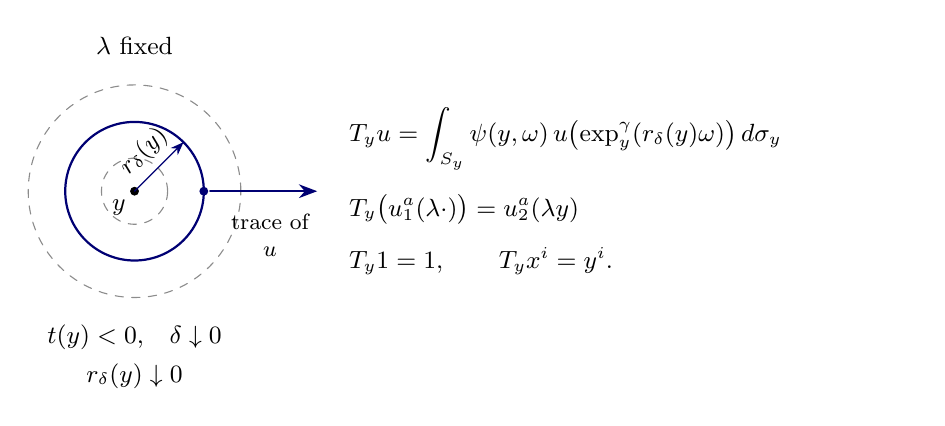
\begin{tikzpicture}[x=1cm,y=1cm,font=\small,>=Stealth,
  line cap=round,line join=round]
  \colorlet{sphereink}{blue!45!black}
  \node at (1.70,2.40) {$\lambda$ fixed};
  \draw[black!45,dashed] (1.70,0.55) circle (1.35);
  \draw[sphereink,thick] (1.70,0.55) circle (0.88);
  \draw[black!45,dashed] (1.70,0.55) circle (0.42);
  \fill (1.70,0.55) circle (1.6pt);
  \node[anchor=north east,inner sep=3pt] at (1.70,0.55) {$y$};
  \draw[->,sphereink] (1.70,0.55)--(2.3223,1.1723);
  \node[rotate=45,anchor=south,inner sep=3pt] at (2.011,0.861) {$r_\delta(y)$};
  \fill[sphereink] (2.58,0.55) circle (1.6pt);
  \draw[->,sphereink,thick] (2.66,0.55)--(4.02,0.55);
  \node[anchor=north,align=center,font=\footnotesize] at (3.42,0.38)
    {trace of\\$u$};
  \node[anchor=north,align=center] at (1.70,-1.02)
    {$t(y)<0$,\quad $\delta\downarrow0$\\[3pt]
     $r_\delta(y)\downarrow0$};
  \node[anchor=west,align=left,text width=7.10cm] at (4.30,0.55) {
    $\displaystyle
      T_yu=\int_{S_y}\psi(y,\omega)\,
        u\bigl(\exp_y^\gamma(r_\delta(y)\omega)\bigr)
        \,d\sigma_y$\\[8pt]
    $T_y\bigl(u_1^a(\lambda\cdot)\bigr)=u_2^a(\lambda y)$\\[8pt]
    $T_y1=1,\qquad T_yx^i=y^i.$
  };
\end{tikzpicture}
\caption{A two-dimensional section of the spheres
$d_\gamma(x,y)=r_\delta(y)$ in normal coordinates at $y$ for $t(y)<0$,
with $\lambda$ fixed and $\delta\downarrow0$.
The arrow indicates the trace of $u$ used in
\eqref{balls:density-representation}. Equation~\eqref{balls:reproduction}
gives $T_y\bigl(u_1^a(\lambda\cdot)\bigr)=u_2^a(\lambda y)$,
$T_y1=1$, and $T_yx^i=y^i$.
The measure $d\sigma_y$ has total mass one, and $\psi$ need not be positive.}
\label{fig:shrinking-functional}
\end{figure}
\section{An estimate on the shrinking spheres}
\label{sec:angular}

Proposition~\ref{balls:functional} represents $T_y$ by the density
$\psi$ for every positive radius.
We now prove the bound \eqref{local:density-bound}, uniform as
$\delta\downarrow0$.
The equation $P\psi=0$ in \eqref{angular:P-equation} contains
derivatives in the center variable $y$ and the sphere variable $\omega$.
Lemma~\ref{angular:raising} compares the operators $T$ and $T^\flat$
defined in \eqref{angular:T-definition}.
Proposition~\ref{angular:coercivity} then includes the second-order
terms of $P$ using \eqref{angular:norm-comparison}.

\subsection{The equation for the density}

Use $\gamma,Q,h$ from \eqref{balls:normalization} and write
$r=r_\delta$, $f=f_\delta$, and $\beta=\beta_\delta$ from
\eqref{balls:radius}. The bounds in \eqref{balls:profile-estimates},
together with the uniform $C^m$ bounds for $\gamma$, $\gamma^{-1}$,
and $Q$ on a fixed neighborhood of $Y$ from Subsection~\ref{balls:setup},
give
\begin{equation}\label{angular:profile-bounds}
 \beta\ge\beta_0,\qquad
 \operatorname{Hess}_\gamma f\le-c_0\beta\gamma,
 \qquad |\nabla^j f|\le C_j\beta^j\quad(1\le j\le8),
\end{equation}
where $\nabla^j f$ is taken with the $\gamma$ connection. The
bound $\beta_0$ can be made arbitrarily large by choosing $p$
since $\beta_\delta\ge cp$ in \eqref{balls:profile-estimates}. In passing
from coordinate to covariant derivatives, lower powers of $\beta$
are bounded by $\beta^j$ for $\beta\ge1$.

Write $S_\gamma Y=\{(y,\omega):y\in Y,\ \omega\in S_y\}$, where
$S_y$ and $d\sigma_y$ are the unit sphere and probability measure
used in \eqref{balls:density-representation}. The derivative $\nabla$
varies $y$ with $\omega$ transported parallel for $\gamma$ and acts
covariantly on tensor indices.
This parallel transport preserves $d\sigma_y$. Norms and adjoints
on $S_\gamma Y$ use $dV_\gamma(y)\,d\sigma_y(\omega)$.

For $v$ on $S_y$, let $V$ be its harmonic extension to the unit ball
in $(T_y\mathbb R^n,\gamma_y)$ with the constant metric $\gamma_y$.
In an orthonormal frame, set $Bv(\omega)=\omega\cdot\nabla_z V(\omega)$
and $A_iv(\omega)=\partial_{z_i}V(\omega)$. On spherical harmonics
$\mathcal H_k$ of degree $k$, $Bv=kv$ and
$A_i\mathcal H_k\subset\mathcal H_{k-1}$ for $k\ge1$, while $A_i1=0$.
Write $A_i^*$ for the adjoint on $L^2(S_y,d\sigma_y)$.
Orthogonal changes of frame preserve the Dirichlet problem, so
$\gamma$-parallel transport commutes with $B$ and transports the
indices of $(A_i)$ with the frame. The operators satisfy
\begin{equation}\label{angular:elementary-identities}
 [B,A_i^*]=A_i^*,\qquad \sum_i A_i^*A_i^*=0.
\end{equation}
Indeed $A_i^*\mathcal H_k\subset\mathcal H_{k+1}$, which gives the
commutator. The second identity is the adjoint of
$\sum_i A_iA_iv=(\Delta_zV)|_{S_y}=0$.
For $s\in\mathbb R$, set
\[
 \|v(y,\cdot)\|_s=\|(1+B)^s v(y,\cdot)\|_{L^2(S_y)}.
\]
This is equivalent to the $H^s(S_y)$ norm since $B$ acts by $k$
and $-\Delta_{S_y}$ by $k(k+n-2)$ on $\mathcal H_k$. For tensors,
the squared norm sums the squared component norms in an orthonormal frame.

Write $\Psi^m$ for the classical pseudodifferential operators of order
$m$ on $S_y$. Use a fixed finite atlas and partition of unity on the
unit sphere in each orthonormal frame. For $a(y)>0$, a family in
$a\Psi^m$ is one whose quotient by $a(y)$ has uniformly bounded
symbol seminorms and bounds on the smoothing kernels. For each
localized full symbol $b$ of the quotient and every $\alpha,\nu$,
the seminorm
\[
 \sup_{\omega,\xi}\langle\xi\rangle^{-m+|\nu|}
       |\partial_\omega^\alpha\partial_\xi^\nu b(\omega,\xi)|
\]
is uniformly bounded.
For the term homogeneous of degree $m-k$, replace $m$ by $m-k$ and
take $|\xi|\ge1$. For the remainder after $N$ homogeneous terms,
replace $m$ by $m-N$. The smoothing kernels have uniform bounds
for all derivatives in both sphere variables. These seminorms are
at fixed $y$. A bound for $j$ derivatives in $y$ with weight
$a\beta^j$ means that division of the differentiated family by
$a(y)\beta(y)^j$ gives the same symbol and kernel bounds.
In particular, the derivative bounds following \eqref{angular:U-bounds}
mean $\partial_y^\nu U_\alpha\in
\eps\beta^{|\nu|-|\alpha|}\Psi^{2-|\alpha|}$ for $|\nu|\le5$.

For the operators divided by their scalar weights we use
\begin{align*}
 \Psi^1&:H^{1/2}\longrightarrow H^{-1/2},
       &\Psi^1&:H^1\longrightarrow L^2,\\
 \Psi^2&:H^{1/2}\longrightarrow H^{-3/2},
       &\Psi^2&:H^2\longrightarrow L^2,\\
 \Psi^3&:H^{3/2}\longrightarrow H^{-3/2}.
\end{align*}
The bounds into $H^{-1/2}$ and $H^{-3/2}$ apply to the coefficients
of $\partial_y^2$, $\partial_y$, and the term with no $y$ derivative
in \eqref{angular:error-types}. The $H^1\to L^2$ bound applies to $J$
in \eqref{angular:P-decomposition} and to $A_i^*$ and the $U_\alpha$
with $|\alpha|=1$ from \eqref{angular:U-bounds} in the proof of
\eqref{angular:cutoff-bound}. The
$H^2\to L^2$ bound applies to $U_0 1$ in
$P1=U_0 1+J1$ from \eqref{angular:P-decomposition} and
\eqref{angular:U-bounds}. The symbol and kernel bounds also apply
to the compositions and adjoints in \eqref{angular:error-operator}.
On $S_y$, a commutator with scalar principal symbols has order at
most the sum of the two orders minus one.

\begin{lemma}[Differentiation of $T_yu$]\label{angular:trace}
Use the balls and $T_y$ in \eqref{balls:flux} and
Proposition~\ref{balls:functional}. Assume \eqref{balls:bootstrap-condition}
at $\delta'=\delta$, so that on $Y$
\begin{equation}\label{angular:smallness}
 \sum_{|\alpha|\le8}|\partial_y^\alpha h|\le\eps r,
 \qquad r\beta^2\le\eps.
\end{equation}
If $\Delta_{g_1(\lambda\cdot)}u=0$ near
$\overline{B_\gamma(y_0,r(y_0))}$, set
\[
 U(y,\omega)=u\bigl(\exp_y^\gamma(r(y)\omega)\bigr)
\]
for $y$ near $y_0$. There are operators $\mathcal C_i$ on $S_y$ with
$\nabla_iU=\mathcal C_iU$. Their $L^2(S_y,d\sigma_y)$ adjoints satisfy
\begin{equation}\label{angular:C-expansion}
 \mathcal C_i^*=r^{-1}A_i^*+f_iB+E_i+F_i,
 \qquad E_i\in r\Psi^1,\quad F_i\in\Psi^0,
 \qquad f_i=\nabla_i f.
\end{equation}
For $0\le j\le6$, $\nabla^j(r^{-1}E_i)\in\beta^j\Psi^1$ and
$\nabla^j F_i\in\beta^j\Psi^0$.

Multiplying $\Delta_{g_2(\lambda\cdot)}u=0$ by
$n/\operatorname{tr}(\gamma g_2(\lambda\cdot)^{-1})$ gives
$Q^{ij}\partial_i\partial_j u=0$ in the common harmonic coordinates,
as in \eqref{balls:normalization}. Equivalently,
$Q^{ij}\nabla_i\nabla_j u+b_2^i\nabla_i u=0$ with
$b_2^k=Q^{ij}\Gamma^k_{ij}(\gamma)$, which has uniform $C^m$ bounds
by Subsection~\ref{balls:setup}. If $\psi$ represents $T_y$ as in
\eqref{balls:density-representation}, then
\begin{equation}\label{angular:P-equation}
 P\psi=0,\qquad
 P=r\left[Q^{ij}(\nabla_i+\mathcal C_i^*)
                    (\nabla_j+\mathcal C_j^*)
             +b_2^i(\nabla_i+\mathcal C_i^*)\right].
\end{equation}
The derivatives in \eqref{angular:P-equation} act covariantly on
the tensor indices, and each $\mathcal C_i^*$ acts at fixed $y$.
\end{lemma}

\begin{proof}
Use $e^{2Lt_0}\Delta_{g_1(\lambda\cdot)}u=0$ with second-order
coefficients $\gamma^{-1}$ as in \eqref{balls:normalization}.
Pull back by $z\mapsto\exp_y^\gamma(rz)$ to the unit ball and multiply
by $r^2$. In $\gamma_y$-orthonormal coordinates the new second-order
coefficients are $\delta^{ij}+O(r^2)$ and the first-order coefficients
are $O(r)$. They are smooth in $(y,r)$ and uniformly elliptic down
to $r=0$. The operator from Dirichlet values to the boundary radial
derivative has the expansion
\begin{equation}\label{angular:radial-expansion}
 B+r B_1(y)+r^2 B_2(y,r),\qquad
 B_1\in\Psi^0,\quad B_2\in\Psi^1.
\end{equation}
For the Dirichlet parametrix, use the boundary symbol construction
of \citep[Theorem~1.1(i) and Proposition~3.1]{JoshiLionheart2005}.
The decaying normal root and the successive transport equations
depend smoothly on $(y,r)$. The order-one symbol of the boundary
radial derivative depends only on the principal coefficients and
the differentiating vector $\omega$. At $r=0$ the operator is $B$.
The $r$ derivative of the principal coefficients vanishes there
and $\omega$ is fixed, so the $r$ derivative of the boundary operator
at $r=0$ has order zero.
Applying the rescaled Dirichlet inverse to the smooth residual of
the parametrix gives the correction to the actual solution.
Uniform Dirichlet estimates for the inverse and its $(y,r)$ derivatives,
followed by Sobolev embedding, give bounds for the smooth kernel of
the correction to the boundary radial derivative. Taylor's formula
in $r$ gives \eqref{angular:radial-expansion} with the stated symbol
and kernel bounds, including for derivatives in $(y,r)$.

For the $y$ derivative in the direction $e_i$ at fixed $r$, transport
$\omega$ parallel along the base curve. The Jacobi field along the
radial geodesic has initial value $e_i$ and initial covariant
derivative zero. At the endpoint
it is $e_i+O(r^2)$ in the parallel frame. The $z$ differential of
$\exp_y^\gamma(rz)$ is $r(I+O(r^2))$ in that frame. Since
$r^{-1}\nabla_i r=f_i$, the vector on the unit ball giving $\nabla_iU$ is
\[
 r^{-1}\bigl(e_i+O(r^2)\bigr)+f_i\omega.
\]
The $O(r^2)$ coefficient divided by $r^2$ is smooth in $(y,r,\omega)$.
Using the $B$ term of \eqref{angular:radial-expansion} for the
radial derivative, $r^{-1}e_i$ and $f_i\omega$ give $r^{-1}A_i$
and $f_iB$, respectively. The $r^{-1}O(r^2)$ coefficient
gives an operator in $r\Psi^1$. By \eqref{angular:radial-expansion}
the terms from $B_1$ are in $\Psi^0$ and those from $B_2$ are in
$r\Psi^1$, using $r|f_i|\le r\beta\le\eps/\beta$ from
\eqref{angular:smallness}. Taking $L^2(S_y,d\sigma_y)$ adjoints
gives \eqref{angular:C-expansion}. Using $r=e^f$, the bounds in
\eqref{angular:profile-bounds} give, for $j\le6$,
$|\nabla^j r|\lesssim r\beta^j$ and
$|\nabla^j f_i|\lesssim\beta^{j+1}$.
Thus $|\nabla^j(r f_i)|\lesssim(r\beta)\beta^j$, and the smooth
$(y,r)$ dependence in \eqref{angular:radial-expansion} gives the
stated derivative bounds for $r^{-1}E_i$ and $F_i$.

By \eqref{balls:density-representation},
$T_yu=\langle\psi(y,\cdot),U(y,\cdot)\rangle_{S_y}$. Since the
$\gamma$-parallel transport preserves $d\sigma_y$ and
$\nabla_iU=\mathcal C_iU$,
\[
 \nabla_i(T_yu)
 =\langle(\nabla_i+\mathcal C_i^*)\psi,U\rangle_{S_y}.
\]
By Proposition~\ref{balls:functional} and \eqref{balls:normalization},
$(Q^{ij}\nabla_i\nabla_j+b_2^i\nabla_i)(T_yu)=0$.
Applying the derivative identity twice and multiplying by $r$
gives $\langle P\psi,U\rangle_{S_y}=0$ for $P$ in
\eqref{angular:P-equation}.
For fixed $y$, solve $\Delta_{g_1(\lambda\cdot)}u=0$ on $B_\gamma(y,r')$
for $r'>r(y)$ with arbitrary smooth Dirichlet data in $\omega$
using $x=\exp_y^\gamma(r'\omega)$. As $r'\downarrow r(y)$, the
traces on $x=\exp_y^\gamma(r(y)\omega)$ converge to those data in
$C^\infty(S_y)$ by smooth dependence of the Dirichlet solution on
$r'$. Hence $P\psi=0$.
\end{proof}

\subsection{Decomposition of \texorpdfstring{$P$}{P}}

Use the hypotheses of Lemma~\ref{angular:trace}, with
\eqref{angular:profile-bounds} and \eqref{angular:smallness}. Set
\begin{equation}\label{angular:T-definition}
 D_i^+=\nabla_i+f_iB,\qquad D_i^-=-\nabla_i+f_iB,
 \qquad
 T=\sum_i A_i^*D_i^+,\quad T^\flat=\sum_i A_iD_i^-.
\end{equation}
On $S_\gamma Y$, $\nabla_i$ and $B$ preserve spherical-harmonic
degree. By the actions of $A_i^*$ and $A_i$ given with
\eqref{angular:elementary-identities}, $T$ sends degree $k$ to $k+1$
and $T^\flat$ sends degree $k\ge1$ to $k-1$. Also $T^\flat$ vanishes
on functions of degree zero.

Use $\nabla_i(r^{-1})=-f_i r^{-1}$ from \eqref{balls:radius}.
Parallel transport preserves $A_j^*$ with its frame index, as
explained before \eqref{angular:elementary-identities}. Hence
\[
 [D_i^+,r^{-1}A_j^*]=r^{-1}f_i([B,A_j^*]-A_j^*)=0
\]
by \eqref{angular:elementary-identities}.
In a $\gamma$-orthonormal frame, the other identity in
\eqref{angular:elementary-identities} gives
$Q^{ij}A_i^*A_j^*=h^{ij}A_i^*A_j^*$ by \eqref{balls:normalization}.
Also $2Q^{ij}A_i^*D_j^+=2T+2h^{ij}A_i^*D_j^+$ by
\eqref{angular:T-definition}. Substituting \eqref{angular:C-expansion}
into \eqref{angular:P-equation} therefore gives
\begin{equation}\label{angular:P-decomposition}
 P=2T+U+J,
\end{equation}
where
\begin{align*}
 J&=Q^{ij}(A_i^*F_j+F_iA_j^*)+b_2^iA_i^*,\\
 U&=\frac{h^{ij}}{r}A_i^*A_j^*
       +2h^{ij}A_i^*D_j^+
       +Q^{ij}(A_i^*E_j+E_iA_j^*)\\
  &\quad+rQ^{ij}(D_i^++E_i+F_i)(D_j^++E_j+F_j)
       +r b_2^i(D_i^++E_i+F_i).
\end{align*}
In the definition before \eqref{angular:elementary-identities},
$A_i$ is the sum of a tangential derivative and $\omega_i B$, so
$A_i^*\in\Psi^1$ by \eqref{angular:radial-expansion}. Since
$F_i\in\Psi^0$ by \eqref{angular:C-expansion} and $Q,b_2$ have
uniform bounds by Subsection~\ref{balls:setup} and
Lemma~\ref{angular:trace}, $J$ acts on each $S_y$ and belongs to
$\Psi^1$ uniformly as $\beta_0$ is increased.

Write $U$ in the coordinates $y$ and identify $S_y$ with the unit
sphere using a smooth $\gamma$-orthonormal frame. In this frame
$\nabla_i$ is a derivative in $y$ along the $i$th frame vector,
with angular first derivatives from parallel transport and
zeroth-order terms on tensor indices. Their coefficients are
bounded by the metric bounds in Subsection~\ref{balls:setup}. Thus $D_i^++E_i+F_i$ has
bounded coefficients of the first derivatives in $y$ and an
operator in $\beta\Psi^1$ at order zero in $y$, by
\eqref{angular:profile-bounds} and \eqref{angular:C-expansion}.
The coefficients of $rQ^{ij}(D_i^++E_i+F_i)(D_j^++E_j+F_j)$
at orders $2,1,0$ in $y$ then belong to
$r\Psi^0$, $r\beta\Psi^1$, and $r\beta^2\Psi^2$, respectively.
The coefficients of $r b_2^i(D_i^++E_i+F_i)$ at orders $1,0$
in $y$ belong to $r\Psi^0$, $r\beta\Psi^1$, respectively.
By \eqref{angular:smallness},
$(h^{ij}/r)A_i^*A_j^*\in\eps\Psi^2$ and the coefficients of
$2h^{ij}A_i^*D_j^+$ at orders $1,0$ in $y$ belong to
$\eps r\Psi^1$, $\eps r\beta\Psi^2$. By \eqref{angular:C-expansion},
$Q^{ij}(A_i^*E_j+E_iA_j^*)\in r\Psi^2$.
Since $r\beta^2\le\eps$ and $\beta\ge1$, these bounds give
\begin{equation}\label{angular:U-bounds}
 U=\sum_{|\alpha|\le2}U_\alpha(y)\partial_y^\alpha,
 \qquad U_\alpha\in\eps\beta^{-|\alpha|}
                               \Psi^{2-|\alpha|}.
\end{equation}
For $|\nu|\le5$, the bounds are
$\partial_y^\nu U_\alpha\in
\eps\beta^{|\nu|-|\alpha|}\Psi^{2-|\alpha|}$.
Indeed, \eqref{angular:profile-bounds} gives
$|\nabla^j r|\lesssim r\beta^j$ and
$|\nabla^j f_i|\lesssim\beta^{j+1}$, while
\eqref{angular:smallness} bounds the derivatives of $h$.
The terms $D_i^+E_j$ and $D_i^+F_j$ use at most six derivatives of
$E_j$ and $F_j$ after applying $\partial_y^\nu$, covered by
Lemma~\ref{angular:trace} following \eqref{angular:C-expansion}.

The terms with two derivatives in $y$ come from
$rQ^{ij}\nabla_i\nabla_j$ in $U$. In coordinates their operator is
\begin{equation}\label{angular:real-principal-part}
 rQ^{ij}\partial_{y_i}\partial_{y_j};
\end{equation}
the coefficients $rQ^{ij}$ are real functions of $y$.

On the right of \eqref{angular:norm-comparison}, use
\eqref{angular:raising-estimate} for $\|T\varphi\|^2-\|T^\flat\varphi\|^2$
and \eqref{angular:error-form-bound} for $\langle\mathcal E\varphi,\varphi\rangle$,
with $\mathcal E$ from \eqref{angular:error-operator}. Both estimates use
\begin{equation}\label{angular:N-definition}
 \mathcal N(\varphi)^2
 =\int_Y\left(
  \|\nabla\varphi\|_0^2+\beta^2\|\varphi\|_1^2
  +\beta^{-1}\|\nabla\varphi\|_{1/2}^2
  +\beta\|\varphi\|_{3/2}^2\right)dV_\gamma.
\end{equation}
In \eqref{angular:error-form-bound}, the terms
$\beta^{-1}\|\nabla\varphi\|_{1/2}^2$ and
$\beta\|\varphi\|_{3/2}^2$ control the quadratic forms of
$\eps\beta^{-1}\Psi^1\partial_y^2$, $\eps\Psi^2\partial_y$, and
$\eps\beta\Psi^3$ in \eqref{angular:error-types}.

\subsection{Comparison of \texorpdfstring{$T$ and $T^\flat$}{T and T-flat}}

The lower bound in \eqref{angular:raising-estimate} for
$\|T\varphi\|^2-\|T^\flat\varphi\|^2$ is used in
\eqref{angular:norm-comparison}.

\begin{lemma}[Lower bound for $\|T\varphi\|^2-\|T^\flat\varphi\|^2$]\label{angular:raising}
Let $n\ge3$ and suppose \eqref{angular:profile-bounds} holds on a fixed
coordinate region with the uniform bounds for $\gamma,\gamma^{-1}$ in
Subsection~\ref{balls:setup}. For $\beta_0$ sufficiently large in
terms of these bounds and the constants in \eqref{angular:profile-bounds},
there is $c>0$ depending only on the same quantities such that
every smooth $\varphi$
compactly supported in $y$ and satisfying
$\int_{S_y}\varphi(y,\omega)\,d\sigma_y(\omega)=0$ for every $y$ obeys
\begin{equation}\label{angular:raising-estimate}
 \|T\varphi\|^2-\|T^\flat\varphi\|^2
       \ge c\,\mathcal N(\varphi)^2.
\end{equation}
\end{lemma}

\begin{proof}
By \eqref{angular:T-definition}, $T$ sends degree $k$ to $k+1$
and $T^\flat$ sends degree $k\ge1$ to $k-1$. Orthogonality of the
degree components reduces \eqref{angular:raising-estimate} to each
$k\ge1$. Represent the component by its homogeneous harmonic
polynomial $v(z)$ of degree $k$, or equivalently its trace-free
symmetric tensor, as in \cite{PSU15,GPSU16}.

In the Fischer inner product the monomials $z^\alpha$ are orthogonal
with squared norm $\alpha!$, so $a_i=\partial_{z_i}$ is adjoint to
multiplication by $z_i$. In the calculation at degree $k$, use
$|\cdot|$ and $\langle\cdot,\cdot\rangle$ for the Fischer norm and
pairing at fixed $y$. The norm $\|\cdot\|$ and pairing $(\cdot,\cdot)$
include integration with $dV_\gamma(y)$. Use real parts in quadratic
forms. For a harmonic homogeneous polynomial of degree $k$,
\[
 |v|^2=N_k\int_{S_y}|v(\omega)|^2\,d\sigma_y(\omega),
 \qquad N_k=n(n+2)\cdots(n+2k-2),\qquad N_0=1.
\]
In the standard real Gaussian integral of $|v(z)|^2$, pairings of two
indices within $v$ or within $\overline v$ give traces and vanish by
$\Delta_z v=0$. Pairings between $v$ and $\overline v$ give the
Fischer squared norm. The Gaussian radial moment of order $2k$ is $N_k$.
See \cite[Equation~(2.1) and Theorem~2.1]{Render08}.

Set $d=k+n/2-1$. On degree $k$, \eqref{angular:T-definition}
gives $D_i^\pm=\pm\nabla_i+k f_i$. Keep $k$ fixed in these operators
when commuting them past $a_j$ below.
For harmonic homogeneous polynomials $q_i$ of degree $k$,
$\Delta_z\sum_i z_iq_i=2\sum_i a_iq_i$ and
$\Delta_z(|z|^2s)=4d\,s$ for $s\in\mathcal H_{k-1}$. Thus the
harmonic part of $\sum_i z_iq_i$ is
$\sum_i z_iq_i-|z|^2\sum_i a_iq_i/(2d)$. It is the Fischer orthogonal
projection because multiplication by $|z|^2$ is adjoint to $\Delta_z$.
Using these adjoints, its squared norm is
\[
 \sum_i|q_i|^2+\operatorname{Re}\sum_{i,j}\langle a_jq_i,a_iq_j\rangle
             -d^{-1}\Bigl|\sum_i a_iq_i\Bigr|^2.
\]
By restriction to $S_y$, $a_i$ gives $A_i$ as defined before
\eqref{angular:elementary-identities}. The $L^2(S_y)$ pairings in
degrees $k+1$ and $k$ divide the Fischer pairings by $N_{k+1}$
and $N_k$, respectively, giving
\[
 A_i^*v=\frac{N_{k+1}}{N_k}
            \left(z_i v-\frac{|z|^2}{2d}a_iv\right).
\]
Use $q_i=D_i^+v$, $N_{k+1}/N_k=2d+2$, and $N_k/N_{k-1}=2d$ in
\eqref{angular:T-definition}. Then $N_k$ times the degree-$k$
contribution to the left side of \eqref{angular:raising-estimate} is
\begin{equation}\label{angular:Fock-difference}
 \begin{split}
 (2d+2)\left[\|D^+v\|^2
   +\sum_{i,j}(a_jD_i^+v,a_iD_j^+v)
   -\frac1d\Bigl\|\sum_i a_iD_i^+v\Bigr\|^2\right]
 -2d\Bigl\|\sum_i a_iD_i^-v\Bigr\|^2.
 \end{split}
\end{equation}

Write $C_{ij}=2k(\operatorname{Hess}_\gamma f)_{ij}$ and
\[
 C[av]=\int_Y\sum_{i,j}C_{ij}\langle a_iv,a_jv\rangle\,dV_\gamma.
\]
Covariant integration by parts with the fixed factor $k f_i$ in
$D_i^\pm$ gives
\begin{align}
 \sum_{i,j}(a_jD_i^+v,a_iD_j^+v)
   &=\Bigl\|\sum_i a_iD_i^-v\Bigr\|^2-C[av]
                                    +O(k^2)\|v\|^2,\label{angular:ibp-one}\\
 \Bigl\|\sum_i a_iD_i^+v\Bigr\|^2
   &\le k\|D^-v\|^2-C[av]+O(k^2)\|v\|^2,\label{angular:ibp-two}\\
 \|D^-v\|^2
   &=\|D^+v\|^2+\int_Y\tr C\,|v|^2\,dV_\gamma.
                                                    \label{angular:ibp-three}
\end{align}
For \eqref{angular:ibp-one} and \eqref{angular:ibp-two}, transport
the frame index of $a_i$ as for $A_i$ before
\eqref{angular:elementary-identities}. After integrating $D_j^+$
by parts, use
\[
 D_j^-D_i^+=D_i^+D_j^--C_{ij}+[\nabla_i,\nabla_j].
\]
Integrating $D_i^+$ by parts now gives
$\|\sum_i a_iD_i^-v\|^2$ in \eqref{angular:ibp-one}. In
\eqref{angular:ibp-two} it gives
$\operatorname{Re}\sum_{i,j}(a_iD_j^-v,a_jD_i^-v)$, bounded by
$\sum_{i,j}\|a_iD_j^-v\|^2=k\|D^-v\|^2$. Here
$\sum_i|a_i w|^2=k|w|^2$ at degree $k$ follows from
$\sum_i z_i a_i w=kw$ and the Fischer adjoints.
In both identities $-C_{ij}$ contributes $-C[av]$.

On the polynomials, $[\nabla_i,\nabla_j]$ is a linear combination
of $z_\ell a_m-z_m a_\ell$ with coefficients bounded by the curvature
of $\gamma$. These operators have norm $O(k)$ in degree at most $k$
by the adjoint relation and $\sum_i|a_iw|^2=k|w|^2$ in degree $k$.
The curvature on the frame indices is bounded as well by
Subsection~\ref{balls:setup}. Thus $\sum_i\|a_iv\|^2=k\|v\|^2$
bounds the commutator forms in \eqref{angular:ibp-one} and
\eqref{angular:ibp-two} by $Ck^2\|v\|^2$. For
\eqref{angular:ibp-three}, the cross terms in $\|D^+v\|^2$ and
$\|D^-v\|^2$ are $-k\int_Y\Delta_\gamma f\,|v|^2\,dV_\gamma$
and its negative, with $\tr C=2k\Delta_\gamma f$.

Substituting \eqref{angular:ibp-one} into
\eqref{angular:Fock-difference} gives
\begin{equation}\label{angular:after-first-ibp}
 \begin{split}
 &(2+2/d)\left[d\|D^+v\|^2
       -\Bigl\|\sum_i a_iD_i^+v\Bigr\|^2-dC[av]\right]\\
 &\qquad+2\Bigl\|\sum_i a_iD_i^-v\Bigr\|^2
                      +O(k^3)\|v\|^2.
 \end{split}
\end{equation}
For the term $-(2+2/d)\|\sum_i a_iD_i^+v\|^2$ in
\eqref{angular:after-first-ibp}, split the coefficient into fractions
$1-\vartheta$ and $\vartheta$, with $\vartheta>0$ small and fixed.
Use \eqref{angular:ibp-two} and \eqref{angular:ibp-three} for
$1-\vartheta$. For $\vartheta$, use the pointwise bound
\begin{equation}\label{angular:convex-bound}
 \begin{split}
 \Bigl|\sum_i a_iD_i^+v\Bigr|^2
 &\le(1-\zeta)(k+n-1)|D^+v|^2\\
 &\quad+\zeta\left(2\Bigl|\sum_i a_iD_i^-v\Bigr|^2
                         +8k^3\beta^2|v|^2\right),
 \qquad \zeta=c_1/\beta.
 \end{split}
\end{equation}
with $c_1>0$ small so that $0<\zeta\le1$. For the term with
$1-\zeta$, use the adjoint of $(q_i)\mapsto\sum_i a_iq_i$ on
homogeneous polynomials, which is $w\mapsto(z_iw)_i$. For $w$ of degree $k-1$,
$\sum_i|z_iw|^2=(k+n-1)|w|^2$ by $\sum_i a_i(z_iw)=(k+n-1)w$.
This gives $|\sum_i a_iD_i^+v|^2\le(k+n-1)|D^+v|^2$.
For the term with $\zeta$, substitute
$D_i^+v=2kf_i v-D_i^-v$ from \eqref{angular:T-definition} and use
$|\sum_i f_i a_i v|^2\le k\beta^2|v|^2$ and $|a-b|^2\le2|a|^2+2|b|^2$.

Using \eqref{angular:ibp-two}, \eqref{angular:ibp-three}, and
\eqref{angular:convex-bound} in \eqref{angular:after-first-ibp}
gives the following coefficient of $|D^+v|^2$
\begin{equation}\label{angular:positive-degree-factor}
 (2+2/d)\bigl[d-k-\vartheta(n-1)
                         +\vartheta\zeta(k+n-1)\bigr].
\end{equation}
Since $d-k=(n-2)/2$, small fixed $\vartheta$ makes
\eqref{angular:positive-degree-factor} bounded below by a positive
constant plus a positive multiple of $c_1 k/\beta$. The coefficient
of $|\sum_i a_iD_i^-v|^2$ is $2-2\vartheta(2+2/d)\zeta\ge0$
for large $\beta_0$. The $C[av]$ terms from
\eqref{angular:after-first-ibp} and \eqref{angular:ibp-two},
together with $\tr C$ from \eqref{angular:ibp-three}, give
\begin{equation}\label{angular:hessian-contribution}
 -(2+2/d)\left[(d-1+\vartheta)C[av]
       +(1-\vartheta)k\int_Y\tr C\,|v|^2\,dV_\gamma\right].
\end{equation}
By \eqref{angular:profile-bounds},
$-C[av]\ge 2c_0 k^2\int_Y\beta|v|^2\,dV_\gamma$
and $-\tr C\ge 2nc_0 k\beta$. Since $d-1+\vartheta\gtrsim k$
for $k\ge1$ and $n\ge3$, \eqref{angular:hessian-contribution} is
bounded below by $c k^3\int_Y\beta|v|^2\,dV_\gamma$. The errors in
\eqref{angular:after-first-ibp} and \eqref{angular:ibp-two} are
bounded by $C k^3\|v\|^2\le C\beta_0^{-1}k^3\int_Y\beta|v|^2\,dV_\gamma$.
The $8\zeta k^3\beta^2$ term in \eqref{angular:convex-bound} has
$\zeta k^3\beta^2=c_1 k^3\beta$. Thus large $\beta_0$ and small $c_1$
allow both contributions to be absorbed by the lower bound.

The expression in \eqref{angular:Fock-difference} is therefore
bounded below by a positive constant times the sum of
\[
 \|D^+v\|^2,\qquad
 \int_Y\frac{k}{\beta}|D^+v|^2\,dV_\gamma,
 \qquad k^3\int_Y\beta|v|^2\,dV_\gamma.
\]
The expansion of $\|D^+v\|^2$ used in \eqref{angular:ibp-three}
gives $\|D^+v\|^2\ge \|\nabla v\|^2+k^2\int_Y\beta^2|v|^2\,dV_\gamma$,
since $\Delta_\gamma f\le0$ by \eqref{angular:profile-bounds}.
Also, by $D_i^+=\nabla_i+kf_i$,
\[
 \frac{k}{\beta}|\nabla v|^2
 \le2\frac{k}{\beta}|D^+v|^2+2k^3\beta|v|^2.
\]
In the $k$th degree, the sphere norms in \eqref{angular:N-definition}
use $(1+B)^s=(1+k)^s$, with $1+k\asymp k$ for $k\ge1$.
Thus division by $N_k$ gives all four terms of
\eqref{angular:N-definition} at this degree. Summing the orthogonal
components proves \eqref{angular:raising-estimate}.
\end{proof}

\subsection{Estimate for \texorpdfstring{$P$}{P}}

For $P=2T+U+J$ in \eqref{angular:P-decomposition}, use
\eqref{angular:norm-comparison} with the bounds
\eqref{angular:raising-estimate} and \eqref{angular:error-form-bound}.
The operator $U$ contains
$rQ^{ij}\partial_{y_i}\partial_{y_j}$ from
\eqref{angular:real-principal-part} and $(h^{ij}/r)A_i^*A_j^*$ from
the expansion after \eqref{angular:P-decomposition}.

\begin{proposition}[Coercive estimate for $P$]
\label{angular:coercivity}
Fix a coordinate region with uniform bounds for $g_1(\lambda\cdot)$,
$\gamma$, and $\gamma^{-1}$ as in Subsection~\ref{balls:setup}, and
fix $c_0,C_j$ in \eqref{angular:profile-bounds}. Use $P$ from
\eqref{angular:P-equation} with $\mathcal C_i^*$ from
\eqref{angular:C-expansion}. For $\beta_0$ sufficiently large and
$\eps_0>0$ sufficiently small in terms of these bounds,
\eqref{angular:profile-bounds} and \eqref{angular:smallness} with
$\eps\le\eps_0$ imply
\begin{equation}\label{angular:coercive-estimate}
 \mathcal N(\varphi)\le C\|P\varphi\|
\end{equation}
with $C$ depending only on the fixed bounds, for every smooth
$\varphi$ compactly supported in $y$ and satisfying
$\int_{S_y}\varphi(y,\omega)\,d\sigma_y(\omega)=0$ for every $y$.
The constants are uniform in $\delta$ for $r=r_\delta$.
The hypothesis on $h$ uses $\partial_y^\alpha h$ for $|\alpha|\le8$
as in \eqref{angular:smallness}.
\end{proposition}

\begin{proof}
Use the formal adjoint $\dagger$ on
$L^2(S_\gamma Y,dV_\gamma(y)\,d\sigma_y(\omega))$.
With $A_i$ transported as before \eqref{angular:elementary-identities},
integration by parts in \eqref{angular:T-definition} gives
$T^\dagger=\sum_i(-A_i\nabla_i+f_i BA_i)$.
Taking the adjoint of $[B,A_i^*]=A_i^*$ in
\eqref{angular:elementary-identities} gives $[A_i,B]=A_i$, so
\begin{equation}\label{angular:Z-definition}
 Z:=T^\flat-T^\dagger=\sum_i f_iA_i.
\end{equation}
Expanding the squared norms with $T^\flat=T^\dagger+Z$ from
\eqref{angular:Z-definition} gives
\begin{equation}\label{angular:norm-comparison}
 \begin{split}
 &\|(2T+U)\varphi\|^2-
                \|(2T^\flat+U^\dagger)\varphi\|^2\\
 &\qquad=4\bigl(\|T\varphi\|^2-\|T^\flat\varphi\|^2\bigr)
                       +\langle\mathcal E\varphi,\varphi\rangle,
 \end{split}
\end{equation}
where
\begin{equation}\label{angular:error-operator}
 \mathcal E=2[T^\dagger,U]+2[U^\dagger,T]+[U^\dagger,U]
                       -2\bigl(UZ+(UZ)^\dagger\bigr).
\end{equation}
The error satisfies
\begin{equation}\label{angular:error-form-bound}
 |\langle\mathcal E\varphi,\varphi\rangle|
                         \le C\eps\mathcal N(\varphi)^2.
\end{equation}

Use $B\in\Psi^1$ from \eqref{angular:radial-expansion} and
$A_i,A_i^*\in\Psi^1$ as in the calculation after
\eqref{angular:P-decomposition}. By \eqref{angular:T-definition}
and \eqref{angular:Z-definition}, the coefficients of
$\partial_y^\alpha$ in $T,T^\dagger$ belong to
$\beta^{1-|\alpha|}\Psi^{2-|\alpha|}$ for $|\alpha|\le1$, and
$Z\in\beta\Psi^1$. Their derivatives in $y$ use
$|\nabla^j f_i|\lesssim\beta^{1+j}$ from \eqref{angular:profile-bounds}
and the uniform bounds for the frame coefficients. For $U$ use \eqref{angular:U-bounds} and
$\partial_y^\nu U_\alpha\in
\eps\beta^{|\nu|-|\alpha|}\Psi^{2-|\alpha|}$ for $|\nu|\le5$.
The same coefficient bounds hold for $U^\dagger$ because a $y$
derivative hitting a coefficient reduces the number of derivatives
on $\varphi$ by one and adds at most a factor $\beta$.

In the commutators in \eqref{angular:error-operator}, terms with a
$y$ derivative on a coefficient lose at least one derivative on $\varphi$.
Terms with all $y$ derivatives on $\varphi$ have coefficients that
are commutators on $S_y$, so the products of the scalar principal
symbols cancel. Thus the coefficients of $\partial_y^\alpha$ in
$[T^\dagger,U]$ and $[U^\dagger,T]$ belong to
$\eps\beta^{1-|\alpha|}\Psi^{3-|\alpha|}$. The same order bound
holds for $[U^\dagger,U]$ with weight $\eps^2\beta^{-|\alpha|}$,
bounded by $\eps\beta^{1-|\alpha|}$ since $\eps\le1$ and $\beta\ge1$.
The same bounds $\eps\beta^{1-|\alpha|}\Psi^{3-|\alpha|}$ hold
for $UZ$ and $(UZ)^\dagger$ by $Z\in\beta\Psi^1$.

In the coordinates $y$ of \eqref{angular:U-bounds}, identify the
spheres by a smooth $\gamma$-orthonormal frame. The sphere measure
is fixed and the $y$ measure is $(\det\gamma)^{1/2}\,dy$.
The adjoint of the term in \eqref{angular:real-principal-part} is
\[
 \bigl(rQ^{ij}\partial_{y_i}\partial_{y_j}\bigr)^\dagger
 =(\det\gamma)^{-1/2}\partial_{y_j}\partial_{y_i}
       \bigl((\det\gamma)^{1/2}rQ^{ij}\,\cdot\bigr).
\]
Consequently $U^\dagger-U$ has at most one $y$ derivative.
In $[T^\dagger,U]$ and $[U^\dagger,T]$, the coefficients of
three $y$ derivatives are commutators of angular operators with
$rQ^{ij}(y)$, and vanish by \eqref{angular:real-principal-part}.
In $[U^\dagger,U]=[U^\dagger-U,U]$, the coefficients of three
$y$ derivatives vanish for the same reason, using the coefficients
of one $y$ derivative in $U^\dagger-U$. Since $Z$ acts on $S_y$,
$UZ$ and $(UZ)^\dagger$ have at most two $y$ derivatives. We obtain
the following bounds for the terms in $\mathcal E$ by $y$ order
\begin{equation}\label{angular:error-types}
 \eps\beta^{-1}\Psi^1\partial_y^2,
 \qquad \eps\Psi^2\partial_y,
 \qquad \eps\beta\Psi^3.
\end{equation}

Integrate the $\eps\beta^{-1}\Psi^1\partial_y^2$ terms of
\eqref{angular:error-types} once in $y$. Using
$\Psi^1:H^{1/2}(S_y)\to H^{-1/2}(S_y)$ as before
Lemma~\ref{angular:trace}, the pairing of two first derivatives
is bounded by
$C\eps\int_Y\beta^{-1}\|\partial_y\varphi\|_{1/2}^2\,dV_\gamma$.
A derivative on the coefficient gives terms in
$\eps\Psi^1\partial_y$. In particular,
$d\beta=\operatorname{Hess}_\gamma f(\nabla^\gamma f,\cdot)/\beta$
and \eqref{angular:profile-bounds} give
$|d\beta|\lesssim\beta^2$ and $|d(\beta^{-1})|\lesssim1$.

For $\eps\Psi^2\partial_y$ in \eqref{angular:error-types}, including
the terms in $\eps\Psi^1\partial_y$ just obtained, the mapping
$\Psi^2:H^{1/2}(S_y)\to H^{-3/2}(S_y)$ gives the bound
\[
 C\eps\int_Y
     \|\partial_y\varphi\|_{1/2}\|\varphi\|_{3/2}\,dV_\gamma
 \le C\eps\int_Y\left(
     \beta^{-1}\|\partial_y\varphi\|_{1/2}^2
                 +\beta\|\varphi\|_{3/2}^2\right)dV_\gamma.
\]
For $\eps\beta\Psi^3$ use $\Psi^3:H^{3/2}(S_y)\to H^{-3/2}(S_y)$
to get $C\eps\int_Y\beta\|\varphi\|_{3/2}^2\,dV_\gamma$.
In the frame used for \eqref{angular:U-bounds}, the difference
between $\partial_y$ and the coordinate components of $\nabla$
is first order in $\omega$ with bounded coefficients. Hence
$\|\partial_y\varphi\|_{1/2}\lesssim
\|\nabla\varphi\|_{1/2}+\|\varphi\|_{3/2}$.
Since $\beta^{-1}\le\beta$, the bounds are controlled by
$\mathcal N(\varphi)^2$ in \eqref{angular:N-definition}.
Derivatives of a fixed partition of unity in $y$ contribute terms
in $\eps\Psi^2\partial_y$ and $\eps\beta\Psi^3$ of
\eqref{angular:error-types}, using $\beta\ge1$. This proves
\eqref{angular:error-form-bound}.

Choose $\eps_0$ so that $C\eps_0\le2c$, where $C$ is from
\eqref{angular:error-form-bound} and $c$ from
\eqref{angular:raising-estimate}. Equations
\eqref{angular:norm-comparison}, \eqref{angular:raising-estimate},
and \eqref{angular:error-form-bound} then give
\[
 \|(2T+U)\varphi\|^2-
 \|(2T^\flat+U^\dagger)\varphi\|^2
 \ge2c\mathcal N(\varphi)^2.
\]
In particular, $\mathcal N(\varphi)\le C\|(2T+U)\varphi\|$.
In \eqref{angular:P-decomposition}, $J\in\Psi^1$ uniformly as
$\beta_0$ increases. By \eqref{angular:N-definition},
\[
 \|J\varphi\|\le C\|\varphi\|_{L^2(Y;H^1(S_y))}
                         \le C\beta_0^{-1}\mathcal N(\varphi).
\]
Since $(2T+U)\varphi=P\varphi-J\varphi$, we obtain
$\mathcal N(\varphi)\le C\|P\varphi\|+C\beta_0^{-1}\mathcal N(\varphi)$.
Choose $\beta_0$ so that $C\beta_0^{-1}\le1/2$ to give
\eqref{angular:coercive-estimate}.

By \eqref{balls:normalization} and Lemma~\ref{angular:trace},
$Q=\gamma^{-1}+h$ and $b_2^k=Q^{ij}\Gamma^k_{ij}(\gamma)$.
The construction in Lemma~\ref{angular:trace} uses $g_1(\lambda\cdot)$
and $r$ to obtain $\mathcal C_i^*$ in \eqref{angular:C-expansion}.
In \eqref{angular:P-equation}, the dependence on $h$ is through
$Q^{ij}$ and $b_2^i$ multiplying the composed operators. Thus
the $U_\alpha$ in \eqref{angular:U-bounds} depend affinely on $h$
and contain at most one $y$ derivative of $\mathcal C_i^*$.

Forming $U^\dagger$ from \eqref{angular:U-bounds} takes at most
two derivatives of $U_\alpha$. The products in
\eqref{angular:error-operator} take at most two more, and the
integration by parts in $\eps\beta^{-1}\Psi^1\partial_y^2$ in
\eqref{angular:error-types} takes at most one more. The five
derivatives of $U_\alpha$ use up to five derivatives of $h$
and six of $\mathcal C_i^*$. These derivatives are controlled by
\eqref{angular:smallness}, \eqref{angular:profile-bounds}, and the
bounds following \eqref{angular:C-expansion} in Lemma~\ref{angular:trace}.
Since $h=h(y)$, angular symbol seminorms differentiate the
angular factors multiplying $h$.
\end{proof}

\subsection{Uniform bound for \texorpdfstring{$\chi\psi$}{chi psi}}

Use $r=r_\delta$ from \eqref{balls:radius} and
$\chi\in C_c^\infty(Y^\circ)$ from \eqref{balls:cutoff-region}.
Since $B1=\nabla_i1=0$, \eqref{angular:T-definition} gives $T1=0$.
Equations \eqref{angular:P-decomposition} and
\eqref{angular:U-bounds} therefore give $P1=U_0 1+J1$.
Using $U_0\in\eps\Psi^2$ in \eqref{angular:U-bounds} and
$J\in\Psi^1$ as after \eqref{angular:P-decomposition}, the maps
$\Psi^2:H^2(S_y)\to L^2(S_y)$ and $\Psi^1:H^1(S_y)\to L^2(S_y)$
give $\|P1\|_{L^2(S_\gamma Y)}\le C$ uniformly in $\beta$.

The operator $J$ in \eqref{angular:P-decomposition} commutes with
$\chi(y)$ because it acts on each $S_y$. Equations
\eqref{angular:T-definition}, \eqref{angular:U-bounds}, and
\eqref{angular:real-principal-part} give
\begin{align*}
 [P,\chi]
 ={}&2\sum_i(\nabla_i\chi)A_i^*
      +2rQ^{ij}(\partial_{y_i}\chi)\partial_{y_j}\\
 &+rQ^{ij}(\partial_{y_i}\partial_{y_j}\chi)
      +\sum_{|\alpha|=1}(\partial_y^\alpha\chi)U_\alpha.
\end{align*}
Each coefficient here is supported in $\operatorname{supp}(d\chi)$.
By \eqref{angular:U-bounds}, $U_\alpha\in\eps\beta^{-1}\Psi^1$ for
$|\alpha|=1$. The map $\Psi^1:H^1(S_y)\to L^2(S_y)$ applies to
these coefficients and to $A_i^*$ in the first term. In the coordinates
used for \eqref{angular:U-bounds}, $\partial_y$ differs from the
coordinate components of $\nabla$ by a first-order angular operator
with bounded coefficients, as in the proof of
\eqref{angular:error-form-bound}. Hence
$\|r\partial_y w\|_{L^2(S_y)}\lesssim
\|r\nabla w\|_{L^2(S_y)}+r\|w\|_{H^1(S_y)}$.
Use the uniform bound on $Q$ in Subsection~\ref{balls:setup} and
$r\le\eps$ from \eqref{angular:smallness} and
\eqref{angular:profile-bounds} to obtain
\begin{equation}\label{angular:cutoff-bound}
 \|[P,\chi]w\|
 \le C_\chi\left(
  \|w\|_{L^2(\supp d\chi;H^1(S_y))}
    +\|r\nabla w\|_{L^2(\supp d\chi;L^2(S_y))}\right),
\end{equation}

\begin{lemma}[$L^2$ estimate for $\chi\psi$]\label{local:density}
Fix $L$ as in Subsection~\ref{balls:setup} and choose
$p,\varepsilon,R_*$ as in Proposition~\ref{balls:continuation},
with $p$ large and $\varepsilon$ small enough for
Proposition~\ref{angular:coercivity}. Whenever
\eqref{balls:bootstrap-condition} holds, the function $\psi$ in
\eqref{balls:density-representation} satisfies
\begin{equation}\label{local:density-bound}
 \|\chi\psi\|_{L^2(S_\gamma Y)}\leq C
\end{equation}
with $C$ independent of $\delta$ and sufficiently small $\lambda$.
\end{lemma}

\begin{proof}
Set $\varphi=\chi(\psi-1)$. It is compactly supported in $y$, and
$\int_{S_y}\varphi\,d\sigma_y=0$ by \eqref{balls:reproduction}
and $\int_{S_y}d\sigma_y=1$. Equation
\eqref{balls:bootstrap-condition} at $\delta'=\delta$ gives
\eqref{angular:smallness}, so \eqref{angular:coercive-estimate}
applies to $\varphi$. Using $P\psi=0$ in \eqref{angular:P-equation}
gives
\begin{equation}\label{local:density-equation}
 P\varphi=P\bigl(\chi(\psi-1)\bigr)
       =-\chi P1+[P,\chi](\psi-1).
\end{equation}
Proposition~\ref{balls:functional} gives uniform $C^1(S_y)$ bounds
for $\psi$ and $C^0(S_y)$ bounds for $\nabla\psi$ on
$\operatorname{supp}(d\chi)$ in \eqref{balls:cutoff-region}.
Since $r\beta^2\le\eps$ by \eqref{angular:smallness},
\eqref{angular:cutoff-bound} gives
$\|[P,\chi](\psi-1)\|_{L^2(S_\gamma Y)}\le C$.
Together with $\|P1\|_{L^2(S_\gamma Y)}\le C$ this bounds
$\|P\varphi\|$ in \eqref{local:density-equation}.
By \eqref{angular:coercive-estimate}, $\mathcal N(\varphi)\le C$.
The term $\beta^2\|\varphi\|_1^2$ in \eqref{angular:N-definition}
gives $\|\varphi\|_{L^2(S_\gamma Y)}\le\beta_0^{-1}\mathcal N(\varphi)$,
since $\beta\ge\beta_0$ and $\|\varphi\|_1\ge\|\varphi\|_0$.
Since $\chi$ is fixed and $\chi\psi=\varphi+\chi$, this gives
\eqref{local:density-bound}.
\end{proof}

Lemma~\ref{local:moment} uses \eqref{balls:reproduction} and
\eqref{local:density-bound} to obtain \eqref{local:moment-bound}
for $\lambda^{-2}\bigl(u_2^a(\lambda y)-u_1^a(\lambda y)\bigr)$
with weight $\chi/r_\delta^2$.
\section{From harmonic differences to local metric extension}\label{sec:bootstrap}

Lemma~\ref{local:density} gives a uniform $L^2$ bound for $\psi$ in
\eqref{balls:density-representation}.  The constant and coordinate
identities in \eqref{balls:reproduction} imply
\eqref{local:moment-bound}, a uniform $L^2$ bound for
$\lambda^{-2}\bigl(u_2^a(\lambda y)-u_1^a(\lambda y)\bigr)$
with weight $\chi/r_\delta^2$.
The linear system \eqref{local:metric-system} then relates the
second derivatives of those differences to the normalized inverse
metric difference $h$ defined in \eqref{balls:normalization}.
Using the interpolation estimate \eqref{local:interpolation-estimate},
we improve $H_8\le\varepsilon r_\delta$ to
$H_8\le\varepsilon r_\delta/2$.  This allows $\delta\downarrow0$
with the spatial dilation $\lambda$ fixed.

\subsection{Estimates for differences of harmonic functions and \texorpdfstring{$h$}{h}}

For the pairs $(u_1^a,u_2^a)$ in Theorem~\ref{local:extension},
$u_1^a=u_2^a$ on $W$. Since $0\in\overline W$ and the functions
are smooth, $u_1^a(0)=u_2^a(0)$ and $du_1^a(0)=du_2^a(0)$.
In the original coordinates, define
\begin{equation}\label{local:renormalized-pairs}
 v_j^a(z)=u_j^a(z)-u_1^a(0)-du_1^a(0)\cdot z.
\end{equation}
The functions $1,y^i$ are harmonic for $g_j(\lambda\cdot)$ in
the common harmonic coordinates of Subsection~\ref{balls:setup}.
Thus
$\Delta_{g_j(\lambda\cdot)}\bigl(\lambda^{-2}v_j^a(\lambda\cdot)\bigr)=0$,
and $v_1^a(\lambda y)=v_2^a(\lambda y)$ for $y\in W_\lambda$.
Applying $T_y$ to $v_1^a(\lambda\cdot)$ in
\eqref{local:renormalized-pairs} and using \eqref{balls:reproduction} gives
\begin{align*}
 \lambda^{-2}\bigl[T_y\bigl(v_1^a(\lambda\cdot)\bigr)-v_1^a(\lambda y)\bigr]
 &=\lambda^{-2}\bigl(v_2^a(\lambda y)-v_1^a(\lambda y)\bigr)\\
 &=\lambda^{-2}\bigl(u_2^a(\lambda y)-u_1^a(\lambda y)\bigr).
\end{align*}

Since $v_j^a(0)=0$ and $dv_j^a(0)=0$ by
\eqref{local:renormalized-pairs}, Taylor's formula gives
$\lambda^{-2}|v_j^a(\lambda y)|\le C|y|^2$ and
$\lambda^{-1}|dv_j^a(\lambda y)|\le C|y|$ on each fixed bounded
coordinate set. For $|\alpha|\ge2$,
\begin{align*}
 \partial_y^\alpha\bigl(\lambda^{-2}v_j^a(\lambda y)\bigr)
 &=\lambda^{|\alpha|-2}(\partial^\alpha v_j^a)(\lambda y).
\end{align*}
Thus, on each fixed bounded coordinate set and for every fixed $m$,
\begin{equation}\label{local:uniform-Cm-bound}
 \bigl\|\lambda^{-2}v_j^a(\lambda\cdot)\bigr\|_{C^m}\le C_m
 \qquad(j=1,2)
\end{equation}
uniformly for sufficiently small $\lambda$.
Also $(\partial^2v_1^a)(\lambda\cdot)$ converges smoothly to
$\partial^2u_1^a(0)$ as $\lambda\downarrow0$.

\begin{lemma}[$L^2$ bound for the rescaled harmonic differences]\label{local:moment}
Assume \eqref{balls:bootstrap-condition} and use $\chi$ from
\eqref{balls:cutoff-region}. Then
\begin{equation}\label{local:moment-bound}
 \biggl\|\frac{\chi}{r_\delta^2}\,
   \lambda^{-2}\bigl(u_2^a(\lambda y)-u_1^a(\lambda y)\bigr)
 \biggr\|_{L^2(Y)}\leq C
\end{equation}
with a constant independent of $\delta$ and sufficiently small $\lambda$.
\end{lemma}

\begin{proof}
Using $T_y1=1$ and $T_yx^i=y^i$ in \eqref{balls:reproduction},
subtract $v_1^a(\lambda y)+\lambda\,dv_1^a(\lambda y)\cdot(x-y)$ from
$v_1^a(\lambda x)$ in \eqref{balls:density-representation}.
With $x=\exp_y^\gamma(r_\delta(y)\omega)$, this gives
\begin{align*}
 &\lambda^{-2}\bigl(u_2^a(\lambda y)-u_1^a(\lambda y)\bigr)\\
 &=\lambda^{-2}\int_{S_y}\psi(y,\omega)
 \bigl(v_1^a(\lambda x)-v_1^a(\lambda y)
        -\lambda\,dv_1^a(\lambda y)\cdot(x-y)\bigr)\,d\sigma_y(\omega).
\end{align*}
Taylor's formula and the uniform $C^2$ bound
\eqref{local:uniform-Cm-bound} for $\lambda^{-2}v_1^a(\lambda\cdot)$
give a bound of $C|x-y|^2$ for
$\lambda^{-2}$ times the remainder. By the bounds on $\gamma$
in Subsection~\ref{balls:setup},
$|x-y|\lesssim d_\gamma(x,y)=r_\delta(y)$.
Cauchy--Schwarz with $\int_{S_y}d\sigma_y=1$ gives
\begin{align*}
 \lambda^{-2}\bigl|u_2^a(\lambda y)-u_1^a(\lambda y)\bigr|
 &\le C r_\delta(y)^2\|\psi(y,\cdot)\|_{L^2(S_y)}.
\end{align*}
Multiply by $\chi/r_\delta^2$ and take the $L^2(Y)$ norm.
Since $dV_\gamma=(\det\gamma)^{1/2}\,dy\asymp dy$ on $Y$,
\eqref{local:density-bound} in Lemma~\ref{local:density} then gives
\eqref{local:moment-bound}.
\end{proof}

In the common harmonic coordinates, apply the multipliers $e^{2Lt_0}$
and $n/\operatorname{tr}\bigl(\gamma g_2(\lambda\cdot)^{-1}\bigr)$ in
\eqref{balls:normalization} to
$\Delta_{g_j(\lambda\cdot)}\bigl(\lambda^{-2}v_j^a(\lambda\cdot)\bigr)=0$
for $j=1,2$, respectively. This gives
\begin{align*}
 (\gamma^{-1})^{ij}(\partial_{ij}v_1^a)(\lambda y)&=0,
 &Q^{ij}(\partial_{ij}v_2^a)(\lambda y)&=0.
\end{align*}
Subtract the two equations using $h=Q-\gamma^{-1}$ and
\eqref{local:renormalized-pairs}. With $\operatorname{tr}(\gamma Q)=n$
from \eqref{balls:normalization}, this gives
\begin{equation}\label{local:metric-system}
 h^{ij}(\partial_{ij}v_1^a)(\lambda y)
 =-\lambda^{-2}Q^{ij}\partial_{y^i}\partial_{y^j}
     \bigl(u_2^a(\lambda y)-u_1^a(\lambda y)\bigr),
 \qquad \operatorname{tr}(\gamma h)=0.
\end{equation}

By Theorem~\ref{local:extension} and $g_1(0)=I$ from
Subsection~\ref{balls:setup}, the matrices $\partial^2u_1^a(0)$ span
the trace-zero symmetric matrices. Their contractions with a real
symmetric matrix $H=(H^{ij})$, together with $\operatorname{tr}H$,
determine $H$. The use of Hessians of harmonic functions to
determine a metric up to scale also appears in
\citep[Proposition~4.1 and Remark~4.2]{LLS20}.
By \eqref{balls:dilation} and \eqref{balls:normalization}, the trace
$\operatorname{tr}(\gamma H)$ tends to $e^{-2Lt_0}\operatorname{tr}H$,
with $e^{-2Lt_0}$ bounded below on $Y$. The limiting trace and
contractions therefore control $|H|$ uniformly in $y$.
The uniform convergence $\gamma\to e^{-2Lt_0}I$ and
$(\partial^2v_1^a)(\lambda\cdot)\to\partial^2u_1^a(0)$ from
\eqref{local:renormalized-pairs} gives
\[
 |H|\le C\left(
       |\operatorname{tr}(\gamma(y)H)|
          +\sum_a|H^{ij}(\partial_{ij}v_1^a)(\lambda y)|
          \right)
\]
uniformly for $y\in Y$ and sufficiently small $\lambda$.

Apply this inequality with $H=\partial^\alpha h$ after
differentiating \eqref{local:metric-system}. The uniform $C^8$
bounds for $\gamma,Q$ in Subsection~\ref{balls:setup} and the
$C^{10}$ bound \eqref{local:uniform-Cm-bound} for
$\lambda^{-2}v_1^a(\lambda\cdot)$ give
\begin{align*}
 |\partial^\alpha h(y)|\le C\biggl(
 &\lambda^{-2}\sum_a\sum_{|\nu|\le|\alpha|+2}
 \bigl|\partial_y^\nu\bigl(u_2^a(\lambda y)-u_1^a(\lambda y)\bigr)\bigr|\\
 &+\sum_{|\nu|<|\alpha|}|\partial^\nu h(y)|\biggr),
 \qquad |\alpha|\le8.
\end{align*}
Induction on $|\alpha|$ gives
\begin{equation}\label{local:metric-jet-bound}
 H_8(y)\leq C\lambda^{-2}\sum_a\sum_{|\alpha|\leq10}
 \bigl|\partial_y^\alpha\bigl(u_2^a(\lambda y)-u_1^a(\lambda y)\bigr)\bigr|,
\end{equation}
where $H_8=\sum_{|\alpha|\le8}|\partial^\alpha h|$ is as in
\eqref{balls:bootstrap-condition}, with $C$ independent of $\delta$
and sufficiently small $\lambda$.

In Lemma~\ref{local:improvement}, \eqref{local:interpolation-estimate}
combines \eqref{local:moment-bound} with the $C^m$ bounds
\eqref{local:uniform-Cm-bound} to bound the right-hand side of
\eqref{local:metric-jet-bound}.

\begin{lemma}[Pointwise derivative estimate]\label{local:interpolation}
Let $V$ be smooth on a neighborhood of $\overline{B(y,s)}\subset
\mathbb R^n$, with $0<s\leq1$ and $\|V\|_{C^m}\leq A_m$ there.
For every multi-index $\alpha$ of length $j<m$,
\begin{equation}\label{local:interpolation-estimate}
 |\partial^\alpha V(y)|\leq C_{m,n}
 \bigl(s^{-j-n/2}\|V\|_{L^2(B(y,s))}
                          +A_m s^{m-j}\bigr).
\end{equation}
\end{lemma}

\begin{proof}
Expand $V(y+sz)$ at $z=0$ through degree $m-1$ for $|z|\le1$.
The remainder is bounded by $C_{m,n}A_m s^m$. Since
$\|V(y+s\,\cdot)\|_{L^2(B(0,1))}
=s^{-n/2}\|V\|_{L^2(B(y,s))}$, the Taylor polynomial has
$L^2(B(0,1))$ norm at most
$s^{-n/2}\|V\|_{L^2(B(y,s))}+C_{m,n}A_m s^m$.
The Gram matrix of the monomials of degree at most $m-1$ in
$L^2(B(0,1))$ is invertible. Hence the coefficient
$s^j\partial^\alpha V(y)/\alpha!$ of $z^\alpha$ is bounded by
$C_{m,n}$ times the polynomial's $L^2(B(0,1))$ norm.
Dividing by $s^j$ gives \eqref{local:interpolation-estimate}.
\end{proof}

\subsection{Estimate for \texorpdfstring{$H_8$}{H8}}

Choose $\eta$ and integers $p,m$ with
\begin{equation}\label{local:exponents}
 \eta=\frac{1}{20+n},\qquad p>20+n,\qquad
 m\geq 10+\frac{3}{2\eta}.
\end{equation}
Choose $p$ large enough that $\beta_\delta\ge cp$ in
\eqref{balls:profile-estimates} gives the lower bound
$\beta\ge\beta_0$ in \eqref{angular:profile-bounds} required by
Proposition~\ref{angular:coercivity}. The constants below may
depend on $p,\eta,m$, fixed independently of $\lambda,\delta$.

\begin{lemma}[Estimate for small $r_\delta$]\label{local:improvement}
Use \eqref{local:exponents} and $K$ from \eqref{balls:K}.
There are $C>0$ and $\rho_0>0$, independent of $\delta$
and sufficiently small $\lambda$, such that
\eqref{balls:bootstrap-condition} implies
\begin{equation}\label{local:superlinear}
 H_8(y)\leq C r_\delta(y)^{3/2}
 \quad\text{for }y\in K\text{ with }r_\delta(y)<\rho_0.
\end{equation}
\end{lemma}

\begin{proof}
Put $r=r_\delta(y)$ and $s=r^\eta$. The cutoff in
\eqref{balls:cutoff-region} equals one near the compact set $K$.
Choose $0<\rho_0\le1$ so that $B(y,s)\subset\{\chi=1\}$
for $y\in K$ and $r<\rho_0$.
By the Lipschitz bound for $r_\delta^{1/p}$ in
Lemma~\ref{balls:profiles}, for $z\in B(y,s)$,
\[
 r_\delta(z)^{1/p}\le r^{1/p}+Cs\le\tfrac32 r^{1/p}
\]
after reducing $\rho_0$, since $s/r^{1/p}=r^{\eta-1/p}\to0$
by \eqref{local:exponents}. Thus $r_\delta(z)^2\le(3/2)^{2p}r^2$
on this ball. Together with $\chi=1$ there,
\eqref{local:moment-bound} in Lemma~\ref{local:moment} gives
\begin{align*}
 \bigl\|\lambda^{-2}\bigl(u_2^a(\lambda\,\cdot)
                   -u_1^a(\lambda\,\cdot)\bigr)\bigr\|_{L^2(B(y,s))}
 &\le Cr^2.
\end{align*}
Apply \eqref{local:interpolation-estimate} with $s=r^\eta$, using
the preceding $L^2(B(y,s))$ bound and the uniform $C^m$ bounds
\eqref{local:uniform-Cm-bound}. For $|\alpha|\le10$,
\begin{align*}
 \lambda^{-2}\bigl|\partial_y^\alpha
       \bigl(u_2^a(\lambda y)-u_1^a(\lambda y)\bigr)\bigr|
 &\le C_m\bigl(r^{2-\eta(|\alpha|+n/2)}+r^{\eta(m-|\alpha|)}\bigr)\\
 &\le C_m r^{3/2}.
\end{align*}
Here $r<1$, and \eqref{local:exponents} gives
$\eta(10+n/2)=1/2$ and $\eta(m-10)\ge3/2$.
Substitute these derivative bounds into
\eqref{local:metric-jet-bound} to obtain \eqref{local:superlinear}.
\end{proof}

For $y\in K$ with $r_\delta(y)<\rho$, the choice
$0<\rho<\rho_0$ and $C\rho^{1/2}\le\varepsilon/2$ in
\eqref{local:rho-choice} gives $H_8(y)\le\varepsilon r_\delta(y)/2$
by \eqref{local:superlinear}. For $r_\delta(y)\ge\rho$, the bound
$\sup_Y H_8\le\varepsilon\rho/2$ in \eqref{local:one-dilation}
gives $H_8(y)\le\varepsilon r_\delta(y)/2$.

\subsection{Local extension of the isometry}

\begin{proof}[Proof of Theorem~\ref{local:extension}]
Fix the common harmonic coordinates in Subsection~\ref{balls:setup},
with $g_1(0)=g_2(0)=I$. Use the pairs $(u_1^a,u_2^a)$ in
Theorem~\ref{local:extension}, with $\partial^2u_1^a(0)$ spanning
the trace-zero symmetric matrices. Use the dilation
\eqref{cross:dilation}.

Fix $Y$ in Subsection~\ref{balls:setup}, $L$ giving
\eqref{balls:depth-hessian}, and $t$ in \eqref{balls:depth}.
Use $t_b$ chosen before \eqref{balls:K} and $K,\chi$ from
\eqref{balls:K} and \eqref{balls:cutoff-region}. Choose $p,\eta,m$
by \eqref{local:exponents}, with $p$ sufficiently large for
Propositions~\ref{balls:continuation} and \ref{angular:coercivity}.
Choose $\varepsilon$ sufficiently small for both propositions and
then $R_*$ as in Proposition~\ref{balls:continuation}. In particular,
the balls lie in normal neighborhoods and \eqref{balls:radius-smallness}
gives $r_{\delta'}\beta_{\delta'}^2\le\varepsilon$ on $Y$ for all
$0<\delta'\le1$.

By \eqref{balls:radius}, $\min_Y r_1>0$ and
$r_\delta(y)\ge R_*t_b^p$ if $t(y)>t_b$. Thus $d_\gamma(x,y)$
is bounded below on $d_\gamma(x,y)=r_1(y)$ for $y\in Y$ and on
$d_\gamma(x,y)=r_\delta(y)$ for $y\in Y\cap\{t>t_b\}$.
The comparison after \eqref{balls:cutoff-region} gives a uniform
positive lower bound on $|x-y|$ on both sets. Proposition~\ref{cross:initial}
therefore gives uniform $C^m$ bounds for $\mathcal G$ near these
spheres for sufficiently small $\lambda$.

With $C,\rho_0$ from Lemma~\ref{local:improvement}, choose
\begin{equation}\label{local:rho-choice}
 0<\rho<\rho_0,\qquad C\rho^{1/2}\leq\varepsilon/2.
\end{equation}
Fix one sufficiently small $\lambda>0$ so that
$Y\cap\{y_n\le-1/2\}\subset W_\lambda$,
\begin{equation}\label{local:one-dilation}
 \sup_Y H_8\leq\varepsilon\rho/2.
\end{equation}
and
\[
 \sup_Y H_8\le
 \min\left\{\frac{\varepsilon R_*(2t_b)^p}{2},
             \varepsilon\min_Y r_1\right\}.
\]
The inclusion in $W_\lambda$ holds for small $\lambda$ by
Subsection~\ref{balls:setup}. The thresholds for $H_8$ are fixed
and positive, and $H_8\to0$ uniformly by the $C^8$ convergence of
$h$ in Subsection~\ref{balls:setup}. On $W_\lambda$ the metric
equality in \eqref{balls:dilation} gives $h=0$ by
\eqref{balls:normalization}.
Thus $H_8=0$ on $\{y_n<-1/2\}\cap Y$.
On the rest of $Y\setminus K$ we have $t>2t_b$ by \eqref{balls:K},
so $r_\delta\ge R_*(2t_b)^p$ by \eqref{balls:radius}. Thus
$H_8\le\varepsilon r_\delta/2$ on $Y\setminus K$ for all $0<\delta\le1$.
The bound $\sup_Y H_8\le\varepsilon\min_Y r_1$ gives
$H_8\le\varepsilon r_1$ on $Y$.

With $\lambda$ fixed, suppose $H_8\le\varepsilon r_\delta$ on $Y$
for some $0<\delta\le1$. This and $r_{\delta'}\beta_{\delta'}^2
\le\varepsilon$ for all $\delta'\in[\delta,1]$ by
\eqref{balls:radius-smallness} give \eqref{balls:bootstrap-condition}. Lemma~\ref{local:improvement}
and \eqref{local:rho-choice} then give
$H_8\le\varepsilon r_\delta/2$ on $K\cap\{r_\delta<\rho\}$ by
\eqref{local:superlinear}. On $K\cap\{r_\delta\ge\rho\}$,
\eqref{local:one-dilation} gives the same inequality.
Combining with the bound on $Y\setminus K$, we have
\[
 H_8\le\varepsilon r_\delta\text{ on }Y
 \quad\Longrightarrow\quad H_8\le\tfrac12\varepsilon r_\delta
 \text{ on }Y.
\]
By \eqref{balls:radius}, $r_\delta(y)$ is positive and jointly
continuous on $(0,1]\times Y$. Since $Y$ is compact,
$\delta\mapsto\max_Y(H_8/r_\delta)$ is continuous on $(0,1]$.
It is at most $\varepsilon$ at $\delta=1$, and the implication
above prevents it from taking the value $\varepsilon$.
The intermediate value theorem gives $H_8\le\varepsilon r_\delta$
on $Y$ for all $0<\delta\le1$.

Since $t(0)<0$ by \eqref{balls:depth}, $Y^\circ\cap\{t<0\}$ contains
a neighborhood of $0$. By Lemma~\ref{balls:profiles},
$r_\delta\to0$ there as $\delta\downarrow0$. Taking this limit
in $H_8\le\varepsilon r_\delta$ for the fixed $\lambda$ gives
$H_8=0$, hence $h=0$, on that neighborhood.
By \eqref{balls:normalization}, $Q=\gamma^{-1}$ there, so
$g_2(\lambda y)=e^{2\omega(y)}g_1(\lambda y)$ for a smooth $\omega$.
The conformal change of the Laplacian gives
\[
 \Delta_{g_2(\lambda\cdot)}u
 =e^{-2\omega}\bigl(\Delta_{g_1(\lambda\cdot)}u
       +(n-2)\langle d\omega,du\rangle_{g_1(\lambda\cdot)}\bigr).
\]
For each common harmonic coordinate $y^i$ from
Subsection~\ref{balls:setup}, this yields
$(n-2)\langle d\omega,dy^i\rangle_{g_1(\lambda\cdot)}=0$.
As $n\ge3$ and the $dy^i$ form a basis, $d\omega=0$. Also
$g_1(0)=g_2(0)=I$ in these coordinates,
so $\omega(0)=0$ and $\omega=0$ on a connected neighborhood of $0$.
The use of common harmonic functions to determine the conformal
factor appears in \citep[Section~8]{Fuglede1978} and, for a
restricted family, in \citep[Proposition~4.1]{LLS20}.
Thus $g_1(\lambda y)=g_2(\lambda y)$ near $y=0$, which gives
$g_1=g_2$ near $0$ in the original coordinates.
\end{proof}

The order of parameter choices is
\begin{equation}\label{local:parameter-order}
 \begin{gathered}
 (u_1^a,u_2^a)_a,\ (L,Y,t,t_b,K,\chi)
   \;\longrightarrow\;(p,\eta,m)
   \;\longrightarrow\;(\varepsilon,R_*)\\
 \longrightarrow\;\rho\;\longrightarrow\;
 \lambda\text{ fixed}\;\longrightarrow\;\delta\downarrow0.
 \end{gathered}
\end{equation}
Proposition~\ref{global:frontier} applies Theorem~\ref{local:extension}
at a point of $\partial W\cap(M_2^e)^\circ$ to extend the local
isometry $\Phi$ with domain $W$ satisfying \eqref{global:matching}.
\section{The global isometry and the measured boundary}
\label{global:section}

Use $M_j^e$ and $E$ from Proposition~\ref{data:cap},
$U_0\Subset E$, and the evaluations $I_j(p)(f)=u_f^j(p)$ in
\eqref{data:evaluations}. By Lemma~\ref{data:jet-family}(i), $I_j$
is injective and nonzero on $(M_j^e)^\circ$ and zero on
$\partial M_j^e$. Consider smooth local isometries
\[
 \Phi:W\longrightarrow(M_1^e)^\circ,\qquad
 W\subset(M_2^e)^\circ,\qquad \Phi^*g_1=g_2,
\]
where $W$ is connected, open, and contains $E$. Require
\begin{equation}\label{global:matching}
 \Phi|_E=\Id,\qquad I_2(p)=I_1(\Phi(p))\quad(p\in W).
\end{equation}
For $\Phi=\Id$ on $E$, both $\Phi^*g_1=g_2$ and
\eqref{global:matching} follow from Proposition~\ref{data:cap}
and \eqref{data:evaluations}. We use the union of the domains of
these maps as in \citep[Section~6.1]{LLS20}.

\begin{proposition}[Global interior isometry]\label{global:frontier}
There is a surjective isometry
\[
 \Phi:(M_2^e)^\circ\longrightarrow(M_1^e)^\circ
\]
satisfying \eqref{global:matching}.
\end{proposition}

\begin{proof}
Let $W$ be the union of the domains of the local isometries satisfying
\eqref{global:matching} on connected open sets containing $E$.
For two such isometries $\Phi_1,\Phi_2$, \eqref{global:matching} gives
$I_1(\Phi_1(p))=I_1(\Phi_2(p))$ on their overlap. By the injectivity
of $I_1$ in Lemma~\ref{data:jet-family}(i), $\Phi_1(p)=\Phi_2(p)$
there. Thus the maps define a smooth local isometry $\Phi$ on $W$
satisfying \eqref{global:matching}. The union $W$ is connected since
all these connected domains contain $E$. If $\Phi(p)=\Phi(q)$,
\eqref{global:matching} gives $I_2(p)=I_2(q)$, so $p=q$ by
Lemma~\ref{data:jet-family}(i).

For $p\in W$ and $f\in C_c^\infty(U_0)$, equations
\eqref{global:matching}, \eqref{data:evaluations}, and
\eqref{data:green-normalization} give
\begin{align*}
 0&=I_2(p)(f)-I_1(\Phi(p))(f)\\
  &=\int_{U_0}\bigl(G_2(p,q)-G_1(\Phi(p),q)\bigr)f(q)\,dV_{g_1}(q),
\end{align*}
using $g_1=g_2$ on $E$ from Proposition~\ref{data:cap}.
By smoothness of the kernels off their poles and
$\Phi(q)=q$ on $U_0$ from \eqref{global:matching}, the identity for all
$f$ gives $G_2(p,q)-G_1(\Phi(p),\Phi(q))=0$ on $U_0\setminus\{p\}$.
For fixed $p$, symmetry of $G_j$ and \eqref{data:green-normalization} give
\[
 \Delta_{g_2,q}\bigl(G_2(p,q)-G_1(\Phi(p),\Phi(q))\bigr)=0
 \qquad(q\in W\setminus\{p\}),
\]
where we use $\Phi^*g_1=g_2$ and injectivity of $\Phi$ for the
second term. The set $W\setminus\{p\}$ is connected because paths
can be diverted around $p$ in a punctured coordinate ball.
Interior unique continuation from Section~\ref{data:section} gives
\begin{equation}\label{global:green-equality}
 G_2(p,q)=G_1(\Phi(p),\Phi(q)),
             \qquad p,q\in W,\quad p\ne q.
\end{equation}

If $W\ne(M_2^e)^\circ$, choose $p\in\partial W\cap(M_2^e)^\circ$
by connectedness. For any sequence $p_k\in W$ with $p_k\to p$,
compactness gives a subsequence for which $\Phi(p_k)\to q\in M_1^e$.
Equation~\eqref{global:matching} and continuity in
Lemma~\ref{data:jet-family}(i) give $I_2(p)=I_1(q)$.
Lemma~\ref{data:jet-family}(i) gives $I_2(p)\ne0$,
$I_1|_{\partial M_1^e}=0$, and injectivity of $I_1$ in the interior.
Thus $q$ is interior and is uniquely determined by $I_1(q)=I_2(p)$.
Compactness gives $\Phi(p_k)\to q$ whenever $p_k\to p$ in $W$.

Since $\overline{U_0}\subset E\subset W$, we have $p\notin\overline{U_0}$.
If $q\in\overline{U_0}$, then \eqref{global:matching} at $q\in E$
gives $I_2(q)=I_1(q)=I_2(p)$. This would give $p=q\in W$ by
Lemma~\ref{data:jet-family}(i). Thus $q\notin\overline{U_0}$.

By Lemma~\ref{data:jet-family}(ii), choose $f_1,\ldots,f_n\in
C_c^\infty(U_0)$ so that $y=(u_{f_i}^2)_{i=1}^n$ gives harmonic
coordinates near $p$. Set $x=(u_{f_i}^1)_{i=1}^n$.
Equations \eqref{data:evaluations} and \eqref{global:matching} give
$x\circ\Phi=y$ on $W$, and $I_1(q)=I_2(p)$ gives $x(q)=y(p)$.
Using $\Phi^*g_1=g_2$ and $x\circ\Phi=y$ at $p_k\in W$ and then
taking $p_k\to p$ gives
\[
 \langle dy^i,dy^j\rangle_{g_2}(p)
 =\langle dx^i,dx^j\rangle_{g_1}(q).
\]
As the $dy^i(p)$ are linearly independent, so are the $dx^i(q)$.
Thus $x$ gives harmonic coordinates near $q$.

Choose the two coordinate neighborhoods with closures disjoint from
$\overline{U_0}$, and a ball $V$ about $y(p)=x(q)$ in both chart
images. Since $\Phi(p_k)\to q$ whenever $p_k\to p$ in $W$, shrink
$V$ so that $\Phi(W\cap y^{-1}(V))$ lies in the $x$ chart. From
$x\circ\Phi=y$ we obtain $\Phi=x^{-1}\circ y$ on $W\cap y^{-1}(V)$.

Write $g_j,u_f^j,G_j$ in the common coordinates on $V$. The functions
$u_f^j$ are harmonic there since $L_{g_j}u_f^j=f$ and both charts
avoid $\overline{U_0}$. By Lemma~\ref{data:jet-family}(ii), choose
finitely many $f\in C_c^\infty(U_0)$ whose coordinate Hessians
$(\partial_i\partial_j u_f^1)$ form a basis of
$\{H\in\operatorname{Sym}^2(\mathbb R^n):g_1^{ij}H_{ij}=0\}$
at $x(q)$. These Hessians remain linearly independent after
shrinking $V$. Since $\Delta_{g_1}u_f^1=g_1^{ij}\partial_i\partial_j u_f^1=0$
on $V$ in harmonic coordinates, they span the corresponding space
at every point of $V$.

Let $A=y(W\cap y^{-1}(V))$, so $y(p)\in\partial A\cap V$.
Choose $c\in A$ with $|c-y(p)|<\operatorname{dist}(y(p),\partial V)/3$
and set
$r=\operatorname{dist}(c,V\setminus A)$. Since $y(p)\in V\setminus A$,
\[
 0<r\le |c-y(p)|<\operatorname{dist}(c,\partial V).
\]
Since $r<\operatorname{dist}(c,\partial V)$, a sequence approaching
the distance to $V\setminus A$ eventually lies in a compact subset
of $V$. The distance is therefore attained at
$z_*\in\partial B(c,r)\cap(V\setminus A)$.
On $B(c,r)\subset A$, the equalities $\Phi=x^{-1}\circ y$ and
$\Phi^*g_1=g_2$ give $g_1=g_2$ in the common coordinates.
Equations \eqref{data:evaluations} and \eqref{global:matching} give
$u_f^1=u_f^2$ there for every $f\in C_c^\infty(U_0)$.
Equation~\eqref{global:green-equality} gives $G_1=G_2$ for distinct
points of $B(c,r)$. The selected Hessians span
$\{H:g_1^{ij}(z_*)H_{ij}=0\}$ at $z_*$.
Applying Theorem~\ref{local:extension} at $z_*$ with $B(c,r)$ as
the open set on one side of $\partial B(c,r)$ gives $g_1=g_2$
on a neighborhood of $z_*$ in the common coordinates.

Choose a ball about $z_*$ in this neighborhood. There,
$\Delta_{g_2}(u_f^2-u_f^1)=0$, and $u_f^2-u_f^1$ vanishes on the
intersection with $B(c,r)$. Interior unique continuation from
Section~\ref{data:section} gives $u_f^2=u_f^1$ on the ball for every
$f\in C_c^\infty(U_0)$. Thus $x^{-1}\circ y$ is a local isometry
on the preimage of the ball under $y$ and satisfies
$I_2=I_1\circ(x^{-1}\circ y)$ by \eqref{data:evaluations}.
It agrees with $\Phi$ on the overlap since $\Phi=x^{-1}\circ y$
on $W\cap y^{-1}(V)$. The union of these domains is connected
because the ball meets $B(c,r)\subset A$. The extended isometry
satisfies \eqref{global:matching} on this union, which contains
$E$ and $y^{-1}(z_*)$. By the definition of $W$, this would give
$y^{-1}(z_*)\in W$, contradicting $z_*\notin A$.
Hence $W=(M_2^e)^\circ$.

The image $\Phi((M_2^e)^\circ)$ is open in $(M_1^e)^\circ$ since
$\Phi$ is a local diffeomorphism. If $\Phi(p_k)\to q\in(M_1^e)^\circ$,
compactness gives a subsequence with $p_k\to p\in M_2^e$.
Equation~\eqref{global:matching} and continuity in
Lemma~\ref{data:jet-family}(i) give $I_2(p)=I_1(q)\ne0$.
Since $I_2$ vanishes on $\partial M_2^e$ by Lemma~\ref{data:jet-family}(i),
$p$ is interior. Equation~\eqref{global:matching} gives
$I_1(\Phi(p))=I_1(q)$, so $\Phi(p)=q$ by injectivity of $I_1$.
Thus the image is closed in $(M_1^e)^\circ$.
Connectedness gives surjectivity, and injectivity and the local
diffeomorphism property give a smooth inverse.
\end{proof}

\subsection{Boundary extension and restriction to \texorpdfstring{$M$}{M}}

\begin{proposition}[Boundary extension and identity on $\Gamma$]
\label{global:completion}
The isometry of Proposition~\ref{global:frontier} extends to a smooth
diffeomorphism $M_2^e\to M_1^e$. It maps the copy of $M$ in $M_2^e$
onto the copy in $M_1^e$, and its restriction satisfies
\[
 g_2=\Phi^*g_1,\qquad \Phi|_\Gamma=\Id.
\]
\end{proposition}

\begin{proof}
The isometry in Proposition~\ref{global:frontier} preserves the
length distance on the interiors. In $M_j^e$, pushing curves with
interior endpoints off the boundary in a collar leaves the
endpoints fixed and changes their lengths by arbitrarily little.
Thus the length distance on $(M_j^e)^\circ$ agrees with the
restriction of the length distance on $M_j^e$. Compactness and local
comparison with coordinate distances make $M_j^e$ the metric
completion of $(M_j^e)^\circ$. Thus $\Phi$ and its inverse extend
to mutually inverse isometries of the completions. Their interior
restrictions are bijective, so $\Phi(\partial M_2^e)=\partial M_1^e$.

Let $s$ be the distance to $\partial M_j^e$ on each manifold.
In a boundary normal collar $s$ is smooth and $\nabla^{g_j}s$
is the inward unit normal to its level sets. Since $s\circ\Phi=s$
and $\Phi^*g_1=g_2$ in the interior,
$d\Phi(\nabla^{g_2}s)=(\nabla^{g_1}s)\circ\Phi$ there.
Fix a small level $s=s_0>0$ in both collars. In coordinates
$(s,z)$ obtained by flowing along $\nabla^{g_j}s$ from
$z\in\{s=s_0\}$, we have $\Phi(s,z)=(s,\Phi(z))$ for $s>0$.
This expression is smooth at $s=0$, and the same formula applies
to $\Phi^{-1}$.

By \eqref{global:matching} and continuity, $\Phi|_{\overline E}=\Id$.
In the construction of Proposition~\ref{data:cap}, the original
interior in $M_j^e$ is $(M_j^e)^\circ\setminus\overline E$.
Thus $\Phi$ maps these interiors and their closures onto one
another. Its restriction to $M$ satisfies $\Phi^*g_1=g_2$ by
continuity from the interiors. The patch $P_0=\{b>0\}$ in the
construction of Proposition~\ref{data:cap} lies in $\overline E$,
so $\Phi|_{P_0}=\Id$.

For $f\in C_c^\infty(\Gamma)$, extend $f$ by zero to $\partial M$
and use the harmonic solutions $u_f^{g_j}$ on $M$ from
\eqref{intro:energy}. By $\Phi^*g_1=g_2$, both $u_f^{g_2}$ and
$u_f^{g_1}\circ\Phi$ are $g_2$-harmonic. On $P_0$ both have
boundary value $f$ since $\Phi|_{P_0}=\Id$. The map equality in
Theorem~\ref{main:patch} and \eqref{intro:density} give
\[
 (\partial_{\nu_1}u_f^{g_1})\,dS_{g_1}
   =(\partial_{\nu_2}u_f^{g_2})\,dS_{g_2}
   \quad\text{on }P_0.
\]
By Lemma~\ref{data:jets}, $dS_{g_1}=dS_{g_2}$ on $P_0$.
The outward unit normals satisfy $d\Phi\,\nu_2=\nu_1$ there, so
$\partial_{\nu_2}(u_f^{g_1}\circ\Phi)=
\partial_{\nu_1}u_f^{g_1}=\partial_{\nu_2}u_f^{g_2}$ on $P_0$.

Extend $u_f^{g_2}-u_f^{g_1}\circ\Phi$ by zero into $E$.
Its value and normal derivative vanish on $P_0$, so Green's
formula shows that the extension solves $\Delta_{g_2}u=0$
distributionally across $P_0$, as in Section~\ref{data:section}.
Elliptic regularity and unique
continuation on $(M_2^e)^\circ$ give $u_f^{g_2}=u_f^{g_1}\circ\Phi$
on $M$ since the extension vanishes on $E$.
Taking traces gives
\[
 f(q)=f(\Phi(q))\qquad(q\in\partial M,\ f\in C_c^\infty(\Gamma)).
\]
For $q\in\Gamma$ with $\Phi(q)\ne q$, one can choose such an $f$
with $f(q)=1$ and $f(\Phi(q))=0$. Hence $\Phi|_\Gamma=\Id$.
\end{proof}

\begin{proof}[Proof of Theorem~\ref{main:patch}]
The boundary jets in Lemma~\ref{data:jets} give the extensions
$M_j^e$ and the common $E$ in Proposition~\ref{data:cap}.
Proposition~\ref{global:frontier} uses \eqref{global:green-equality}
and the harmonic functions of Lemma~\ref{data:jet-family}(ii) to
apply Theorem~\ref{local:extension}, giving the interior isometry
satisfying \eqref{global:matching}. Proposition~\ref{global:completion}
then gives $\Phi:M\to M$ with $\Phi^*g_1=g_2$ and $\Phi|_\Gamma=\Id$.
All integrals use densities, so the argument requires neither
an orientation nor connectedness of $\partial M$ or $\Gamma$.
\end{proof}
\section{Scalar conductivities on a fixed Euclidean domain}
\label{scalar:section}

Equation~\eqref{scalar:energy-conversion} identifies the conductivity
energy with the metric energy in \eqref{intro:energy}. In the proof
of Corollary~\ref{main:scalar}, Theorem~\ref{main:patch} then gives
$g_2=\Phi^*g_1$ with $\Phi$ fixing a boundary patch. Since
$g_j=\gamma_j^{\,2/(n-2)}e$, $\Phi$ is conformal for $e$.
Lemma~\ref{scalar:boundary-rigidity} gives $\Phi=\Id$.

\begin{lemma}[Conformal diffeomorphisms fixing a boundary patch]
\label{scalar:boundary-rigidity}
Let $\Omega\subset\mathbb R^n$ be a connected open set with smooth
boundary, where $n\ge3$. Suppose $F:\overline\Omega\to\overline\Omega$
is a smooth diffeomorphism of manifolds with boundary and
\[
 F^*e=e^{2b}e\quad\text{in }\Omega
\]
for a real $b\in C^\infty(\overline\Omega)$, where $e$ is the
Euclidean metric. If $F$ fixes a nonempty relatively open subset of
$\partial\Omega$ pointwise, then $F=\Id$ and $b=0$.
\end{lemma}

\begin{proof}
The Christoffel symbols of $e^{2b}e$ are
\[
 \Gamma^k_{ij}=b_i\delta^k_j+b_j\delta^k_i-b_k\delta_{ij},
 \qquad b_i=\partial_i b.
\]
Since $F$ is an isometry from $e^{2b}e$ to $e$,
$\partial_i\partial_jF=\Gamma^k_{ij}\partial_kF$. Substituting
the displayed $\Gamma^k_{ij}$ gives
\begin{equation}\label{scalar:connection}
 D^2F(v,w)
 =DF\bigl(db(v)w+db(w)v-\langle v,w\rangle\nabla b\bigr).
\end{equation}
Smoothness extends \eqref{scalar:connection} to $\partial\Omega$.

Fix a point $q$ of the boundary patch where $F=\Id$ and let $\nu$
be the inward Euclidean unit normal there. For every tangent vector
$v$, differentiating $F=\Id$ along the patch gives $DF(q)v=v$.
Since $F^*e=e^{2b}e$, this gives $b(q)=0$, so $DF(q)$ is orthogonal
and $DF(q)\nu=\pm\nu$. For small $t>0$, $F(q+t\nu)$ lies in $\Omega$,
so its normal velocity $DF(q)\nu$ at $t=0$ points inward.
Hence $DF(q)\nu=\nu$ and $DF(q)=I$.

As $b=0$ on the patch, $db(q)v=0$ for every tangent $v$.
Choose a smooth curve $c$ in the patch with $c(0)=q$ and nonzero
tangent $v=c'(0)$. Twice differentiating $F(c(t))=c(t)$ gives
\[
 D^2F(q)(v,v)+DF(q)c''(0)=c''(0),
\]
so $D^2F(q)(v,v)=0$ by $DF(q)=I$. Equation~\eqref{scalar:connection}
then gives $|v|^2\nabla b(q)=0$, hence $\nabla b(q)=0$.

The metric $e^{2b}e=F^*e$ is flat. Using the displayed
$\Gamma^k_{ij}$, its Ricci tensor satisfies
\[
 0=\operatorname{Ric}_{ij}
 =-(n-2)(b_{ij}-b_i b_j)
   -\bigl(\Delta b+(n-2)|\nabla b|^2\bigr)\delta_{ij},
 \qquad b_{ij}=\partial_i\partial_j b.
\]
Taking the Euclidean trace gives
$\Delta b=-(n-2)|\nabla b|^2/2$. Substituting this into the displayed
equation for $\operatorname{Ric}_{ij}$ and dividing by $n-2$ gives
\begin{equation}\label{scalar:hessian}
 b_{ij}=b_i b_j-\tfrac12|\nabla b|^2\delta_{ij}.
\end{equation}
For \eqref{scalar:connection} and \eqref{scalar:hessian}, see also
\citet[Equations~(4)--(6)]{KushelmanMcGrath2024}.

Along a straight segment of constant velocity $v$,
\eqref{scalar:hessian} gives
\[
 \frac{d}{dt}\nabla b=(\nabla b\cdot v)\nabla b-\tfrac12|\nabla b|^2v.
\]
The right-hand side is locally Lipschitz in $\nabla b$. On a short
inward segment starting at $q$, the initial condition is $\nabla b(q)=0$.
Uniqueness for the displayed equation gives $\nabla b=0$ on this
segment. Since $\Omega$ is connected and open, any point in
$\Omega$ can be joined to the interior endpoint of this segment by
a polygonal path in $\Omega$. Applying uniqueness on each segment
gives $\nabla b=0$ throughout $\Omega$. Since $b(q)=0$, it follows
that $b=0$ on $\overline\Omega$.

Equation~\eqref{scalar:connection} now gives $D^2F=0$ in $\Omega$.
Thus $F$ is affine, and $DF(q)=I$ and $F(q)=q$ give
$F=\Id$ on $\overline\Omega$.
\end{proof}

\begin{proof}[Proof of Corollary~\ref{main:scalar}]
For each conductivity define
\[
 g_j=\gamma_j^{\,2/(n-2)}e.
\]
These are smooth positive metrics on $\overline\Omega$. In Euclidean
coordinates, $g_j^{ab}=\gamma_j^{-2/(n-2)}\delta^{ab}$ and
$dV_{g_j}=\gamma_j^{n/(n-2)}dx$, so
\begin{equation}\label{scalar:energy-conversion}
 \sqrt{\det g_j}\,g_j^{ab}=\gamma_j\delta^{ab},\qquad
 \int_\Omega\langle du,dv\rangle_{g_j}\,dV_{g_j}
       =\int_\Omega\gamma_j\nabla u\cdot\nabla v\,dx.
\end{equation}
Taking $v\in C_c^\infty(\Omega)$ in \eqref{scalar:energy-conversion}
gives the equivalence of $\Delta_{g_j}u=0$ and
$\operatorname{div}(\gamma_j\nabla u)=0$. Thus $u_f^{g_j}=u_f^{\gamma_j}$.
On $\partial\Omega$, $g_j=\gamma_j^{\,2/(n-2)}e$ gives
\[
 \nu_{g_j}=\gamma_j^{-1/(n-2)}\nu_e,\qquad
 dS_{g_j}=\gamma_j^{(n-1)/(n-2)}dS_e,\qquad
 \partial_{\nu_{g_j}}u\,dS_{g_j}
       =\gamma_j\partial_{\nu_e}u\,dS_e.
\]
By \eqref{intro:density} and the definition of $\Lambda_{\gamma_j}^\Gamma$
preceding Corollary~\ref{main:scalar},
\[
 \langle\Lambda_{g_j,\Gamma}f,h\rangle
 =\int_\Gamma h\,\Lambda_{\gamma_j}^\Gamma f\,dS_e,
 \qquad f,h\in C_c^\infty(\Gamma).
\]
The hypothesis of Corollary~\ref{main:scalar} gives equality of these
pairings. By boundedness of the maps in \eqref{intro:energy} and the
approximation following \eqref{intro:density}, this gives
$\Lambda_{g_1,\Gamma}=\Lambda_{g_2,\Gamma}$ on
$H^{1/2}_{co}(\Gamma)$.

Restrict the equal maps to a nonempty relatively open subset of $\Gamma$
proper in $\partial\Omega$. Theorem~\ref{main:patch} gives a smooth
diffeomorphism $\Phi:\overline\Omega\to\overline\Omega$ fixing this
subset pointwise and satisfying $g_2=\Phi^*g_1$. Substituting
$g_j=\gamma_j^{\,2/(n-2)}e$ gives
\[
 \Phi^*e=\Bigl(\frac{\gamma_2}{\gamma_1\circ\Phi}\Bigr)^{2/(n-2)}e.
\]
Lemma~\ref{scalar:boundary-rigidity} gives $\Phi=\Id$. Substituting
this into $g_2=\Phi^*g_1$ gives $\gamma_1=\gamma_2$ on $\overline\Omega$.
\end{proof}

In dimension three, by contrast, two distinct uniformly positive bounded
measurable scalar conductivities on a ball, both equal to one near its
boundary, can have the same full weak Dirichlet-to-Neumann
operator~\cite[Theorem~1.1]{OpenAIRoughScalar2026}.
\begin{filecontents*}[overwrite]{\jobname-references.bib}
@article{AlessandriniGaburro2009,
  author = {Alessandrini, Giovanni and Gaburro, Romina},
  title = {The local {Calder{\`o}n} problem and the determination at the boundary of the conductivity},
  journal = {Communications in Partial Differential Equations},
  volume = {34},
  number = {8},
  year = {2009},
  pages = {918--936},
  doi = {10.1080/03605300903017397},
  eprint = {0807.0848},
  archivePrefix = {arXiv},
  primaryClass = {math.AP},
  url = {https://arxiv.org/abs/0807.0848}
}

@article{AlessandriniKim2012,
  author = {Alessandrini, Giovanni and Kim, Kyoungsun},
  title = {Single-logarithmic stability for the {Calder{\'o}n} problem with local data},
  journal = {Journal of Inverse and Ill-Posed Problems},
  volume = {20},
  number = {4},
  year = {2012},
  pages = {389--400},
  doi = {10.1515/jip-2012-0014},
  eprint = {1202.5485},
  archivePrefix = {arXiv},
  primaryClass = {math.AP},
  url = {https://arxiv.org/abs/1202.5485}
}

@article{BukhgeimUhlmann2002,
  author = {Bukhgeim, Alexander L. and Uhlmann, Gunther},
  title = {Recovering a potential from partial {Cauchy} data},
  journal = {Communications in Partial Differential Equations},
  volume = {27},
  number = {3--4},
  year = {2002},
  pages = {653--668},
  doi = {10.1081/PDE-120002868}
}

@incollection{Calderon1980,
  author = {Calder{\'o}n, Alberto P.},
  title = {On an inverse boundary value problem},
  booktitle = {Seminar on Numerical Analysis and its Applications to Continuum Physics},
  publisher = {Sociedade Brasileira de Matem{\'a}tica},
  address = {Rio de Janeiro},
  year = {1980},
  pages = {65--73},
  note = {Reprinted in Computational \& Applied Mathematics 25 (2006), nos. 2--3, 133--138}
}

@misc{ChenJiangLiuTao2026,
  author = {Lu Chen and Yan Jiang and Hongyu Liu and Longyue Tao},
  title = {Quasianalyticity and geometric rigidity in the anisotropic {Calder{\'o}n} problem},
  year = {2026},
  eprint = {2608.15813},
  archivePrefix = {arXiv},
  primaryClass = {math.AP},
  doi = {10.48550/arXiv.2608.15813},
  url = {https://arxiv.org/abs/2608.15813v2},
  howpublished = {\href{https://arxiv.org/abs/2608.15813v2}{arXiv:2608.15813v2}},
  note = {Preprint, version 2, September 24, 2026}
}

@article{DSFKSU2009,
  author = {{Dos Santos Ferreira}, David and Kenig, Carlos E. and Salo, Mikko and Uhlmann, Gunther},
  title = {Limiting {Carleman} weights and anisotropic inverse problems},
  journal = {Inventiones Mathematicae},
  volume = {178},
  number = {1},
  year = {2009},
  pages = {119--171},
  doi = {10.1007/s00222-009-0196-4},
  eprint = {0803.3508},
  archivePrefix = {arXiv},
  primaryClass = {math.AP},
  url = {https://arxiv.org/abs/0803.3508}
}

@article{DosSantosFerreiraEtAl2009,
  author = {{Dos Santos Ferreira}, David and Kenig, Carlos E. and Sj{\"o}strand, Johannes and Uhlmann, Gunther},
  title = {On the linearized local {Calder{\'o}n} problem},
  journal = {Mathematical Research Letters},
  volume = {16},
  number = {6},
  year = {2009},
  pages = {955--970},
  doi = {10.4310/MRL.2009.v16.n6.a4},
  eprint = {0905.0530},
  archivePrefix = {arXiv},
  primaryClass = {math.AP},
  url = {https://arxiv.org/abs/0905.0530}
}

@article{Fuglede1978,
  author  = {Fuglede, Bent},
  title   = {Harmonic morphisms between {Riemannian} manifolds},
  journal = {Annales de l'Institut Fourier},
  volume  = {28},
  number  = {2},
  year    = {1978},
  pages   = {107--144},
  doi     = {10.5802/aif.691},
  url     = {https://doi.org/10.5802/aif.691}
}

@article{GPSU16,
  author = {Guillarmou, Colin and Paternain, Gabriel P. and Salo, Mikko and Uhlmann, Gunther},
  title = {The {X}-ray transform for connections in negative curvature},
  journal = {Communications in Mathematical Physics},
  volume = {343}, number = {1}, pages = {83--127}, year = {2016},
  doi = {10.1007/s00220-015-2510-x},
  note = {\href{https://arxiv.org/abs/1502.04720v2}{arXiv:1502.04720v2}}
}

@article{GreeneWu1975,
  author  = {Greene, Robert E. and Wu, H.},
  title   = {Embedding of open {Riemannian} manifolds by harmonic functions},
  journal = {Annales de l'Institut Fourier},
  volume  = {25},
  number  = {1},
  year    = {1975},
  pages   = {215--235},
  doi     = {10.5802/aif.549},
  url     = {https://doi.org/10.5802/aif.549}
}

@article{GuillarmouSaBarreto2009,
  author = {Guillarmou, Colin and S{\'a} Barreto, Ant{\^o}nio},
  title = {Inverse problems for {Einstein} manifolds},
  journal = {Inverse Problems and Imaging},
  volume = {3},
  number = {1},
  year = {2009},
  pages = {1--15},
  doi = {10.3934/ipi.2009.3.1},
  url = {https://www.aimsciences.org/article/doi/10.3934/ipi.2009.3.1}
}

@book{HormanderIV2009,
  author = {H{\"o}rmander, Lars},
  title = {The Analysis of Linear Partial Differential Operators {IV}: Fourier Integral Operators},
  series = {Classics in Mathematics},
  publisher = {Springer},
  address = {Berlin, Heidelberg},
  year = {2009},
  doi = {10.1007/978-3-642-00136-9},
  url = {https://link.springer.com/book/10.1007/978-3-642-00136-9},
  note = {Chapter XXVIII}
}

@article{Isakov2007,
  author = {Isakov, Victor},
  title = {On uniqueness in the inverse conductivity problem with local data},
  journal = {Inverse Problems and Imaging},
  volume = {1},
  number = {1},
  year = {2007},
  pages = {95--105},
  doi = {10.3934/ipi.2007.1.95},
  url = {https://www.aimsciences.org/article/doi/10.3934/ipi.2007.1.95}
}

@article{JoshiLionheart2005,
  author = {Joshi, M. S. and Lionheart, W. R. B.},
  title = {An inverse boundary value problem for harmonic differential forms},
  journal = {Asymptotic Analysis},
  volume = {41},
  number = {2},
  year = {2005},
  pages = {93--106},
  doi = {10.3233/ASY-2005-660},
  eprint = {math/9911212},
  archivePrefix = {arXiv},
  primaryClass = {math.AP},
  url = {https://eprints.maths.manchester.ac.uk/1046/1/Joshi-Lionheart-k-form-published.pdf}
}

@article{KenigSalo2013,
  author = {Kenig, Carlos E. and Salo, Mikko},
  title = {The {Calder{\'o}n} problem with partial data on manifolds and applications},
  journal = {Analysis \& PDE},
  volume = {6},
  number = {8},
  year = {2013},
  pages = {2003--2048},
  doi = {10.2140/apde.2013.6.2003},
  url = {https://msp.org/apde/2013/6-8/p07.xhtml}
}

@article{KenigSjostrandUhlmann2007,
  author = {Kenig, Carlos E. and Sj{\"o}strand, Johannes and Uhlmann, Gunther},
  title = {The {Calder{\'o}n} problem with partial data},
  journal = {Annals of Mathematics},
  series = {2},
  volume = {165},
  number = {2},
  year = {2007},
  pages = {567--591},
  doi = {10.4007/annals.2007.165.567},
  url = {https://annals.math.princeton.edu/2007/165-2/p05}
}

@article{KochTataru2005,
  author = {Koch, Herbert and Tataru, Daniel},
  title = {Dispersive estimates for principally normal pseudodifferential operators},
  journal = {Communications on Pure and Applied Mathematics},
  volume = {58},
  number = {2},
  year = {2005},
  pages = {217--284},
  doi = {10.1002/cpa.20067},
  url = {https://math.berkeley.edu/~tataru/papers/oi.pdf}
}

@article{KohnVogelius1984,
  author = {Kohn, Robert V. and Vogelius, Michael},
  title = {Determining conductivity by boundary measurements},
  journal = {Communications on Pure and Applied Mathematics},
  volume = {37},
  number = {3},
  year = {1984},
  pages = {289--298},
  doi = {10.1002/cpa.3160370302}
}

@article{KushelmanMcGrath2024,
  author  = {Kushelman, Mathew and McGrath, Peter},
  title   = {On {Liouville}'s Theorem for Conformal Maps},
  journal = {The American Mathematical Monthly},
  volume  = {131},
  number  = {7},
  year    = {2024},
  pages   = {619--623},
  doi     = {10.1080/00029890.2024.2344409},
  url     = {https://doi.org/10.1080/00029890.2024.2344409}
}

@article{LLS20,
  author  = {Lassas, Matti and Liimatainen, Tony and Salo, Mikko},
  title   = {The {Poisson} embedding approach to the {Calder\'on} problem},
  journal = {Mathematische Annalen},
  volume  = {377},
  number  = {1--2},
  year    = {2020},
  pages   = {19--67},
  doi     = {10.1007/s00208-019-01818-3},
  url     = {https://doi.org/10.1007/s00208-019-01818-3}
}

@article{LassasTaylorUhlmann2003,
  author = {Lassas, Matti and Taylor, Michael and Uhlmann, Gunther},
  title = {The {Dirichlet-to-Neumann} map for complete {Riemannian} manifolds with boundary},
  journal = {Communications in Analysis and Geometry},
  volume = {11},
  number = {2},
  year = {2003},
  pages = {207--221},
  doi = {10.4310/CAG.2003.v11.n2.a2}
}

@article{LassasUhlmann2001,
  author = {Lassas, Matti and Uhlmann, Gunther},
  title = {On determining a {Riemannian} manifold from the {Dirichlet-to-Neumann} map},
  journal = {Annales scientifiques de l'{\'E}cole Normale Sup{\'e}rieure},
  series = {4},
  volume = {34},
  number = {5},
  year = {2001},
  pages = {771--787},
  doi = {10.1016/S0012-9593(01)01076-X},
  url = {https://www.numdam.org/articles/10.1016/s0012-9593(01)01076-x/}
}

@article{Lax1956,
  author = {Lax, Peter D.},
  title = {A stability theorem for solutions of abstract differential equations, and its application to the study of the local behavior of solutions of elliptic equations},
  journal = {Communications on Pure and Applied Mathematics},
  volume = {9},
  number = {4},
  year = {1956},
  pages = {747--766},
  doi = {10.1002/cpa.3160090407},
  url = {https://doi.org/10.1002/cpa.3160090407}
}

@article{LeeUhlmann1989,
  author = {Lee, John M. and Uhlmann, Gunther},
  title = {Determining anisotropic real-analytic conductivities by boundary measurements},
  journal = {Communications on Pure and Applied Mathematics},
  volume = {42},
  number = {8},
  year = {1989},
  pages = {1097--1112},
  doi = {10.1002/cpa.3160420804},
  url = {https://onlinelibrary.wiley.com/doi/10.1002/cpa.3160420804}
}

@misc{Lin2026,
  author = {Yi-Hsuan Lin},
  title = {The anisotropic {Calder{\'o}n} problem: rigidity near the {Euclidean} metric},
  year = {2026},
  eprint = {2609.17261},
  archivePrefix = {arXiv},
  primaryClass = {math.AP},
  doi = {10.48550/arXiv.2609.17261},
  url = {https://arxiv.org/abs/2609.17261v1},
  howpublished = {\href{https://arxiv.org/abs/2609.17261v1}{arXiv:2609.17261v1}},
  note = {Preprint, version 1, September 15, 2026}
}

@article{Malgrange1956,
  author = {Malgrange, Bernard},
  title = {Existence et approximation des solutions des {\'e}quations aux d{\'e}riv{\'e}es partielles et des {\'e}quations de convolution},
  journal = {Annales de l'Institut Fourier},
  volume = {6},
  year = {1956},
  pages = {271--355},
  doi = {10.5802/aif.65},
  url = {https://aif.centre-mersenne.org/articles/10.5802/aif.65/}
}

@article{PSU15,
  author = {Paternain, Gabriel P. and Salo, Mikko and Uhlmann, Gunther},
  title = {Invariant distributions, {Beurling} transforms and tensor tomography in higher dimensions},
  journal = {Mathematische Annalen},
  volume = {363}, number = {1--2}, pages = {305--362}, year = {2015},
  doi = {10.1007/s00208-015-1169-0},
  note = {\href{https://arxiv.org/abs/1404.7009v2}{arXiv:1404.7009v2}}
}

@article{Render08,
  author = {Render, Hermann},
  title = {Reproducing kernels for polyharmonic polynomials},
  journal = {Archiv der Mathematik},
  volume = {91}, number = {2}, pages = {136--144}, year = {2008},
  doi = {10.1007/s00013-008-2447-9},
  note = {\href{https://hdl.handle.net/10197/5499}{Author manuscript}}
}

@article{RulandSalo2019,
  author = {R{\"u}land, Angkana and Salo, Mikko},
  title = {Quantitative {Runge} approximation and inverse problems},
  journal = {International Mathematics Research Notices},
  volume = {2019},
  number = {20},
  year = {2019},
  pages = {6216--6234},
  doi = {10.1093/imrn/rnx301},
  eprint = {1708.06307},
  archivePrefix = {arXiv},
  primaryClass = {math.AP},
  url = {https://doi.org/10.1093/imrn/rnx301}
}

@misc{Stefanov2026,
  author = {Mu{\~n}oz-Thon, Sebasti{\'a}n and Stefanov, Plamen},
  title = {Local rigidity of conformally {Euclidean} metrics for the anisotropic {Calder{\'o}n} problem},
  year = {2026},
  eprint = {2609.13400},
  archivePrefix = {arXiv},
  primaryClass = {math.AP},
  doi = {10.48550/arXiv.2609.13400},
  url = {https://arxiv.org/abs/2609.13400v3},
  howpublished = {\href{https://arxiv.org/abs/2609.13400v3}{arXiv:2609.13400v3}},
  note = {Preprint, version 3, September 27, 2026}
}

@article{SylvesterUhlmann1987,
  author = {Sylvester, John and Uhlmann, Gunther},
  title = {A global uniqueness theorem for an inverse boundary value problem},
  journal = {Annals of Mathematics},
  series = {2},
  volume = {125},
  number = {1},
  year = {1987},
  pages = {153--169},
  doi = {10.2307/1971291},
  url = {https://annals.math.princeton.edu/1987/125-1/p04}
}

@article{Zeriahi1982,
  author = {Z{\'e}riahi, Ahmed},
  title = {Bases communes dans certains espaces de fonctions harmoniques et fonctions s{\'e}par{\'e}ment harmoniques sur certains ensembles de $\mathbf{C}^n$},
  journal = {Annales de la Facult{\'e} des sciences de Toulouse: Math{\'e}matiques},
  series = {5}, volume = {4}, number = {1}, year = {1982}, pages = {75--102},
  doi = {10.5802/afst.575},
  note = {\href{https://doi.org/10.5802/afst.575}{Journal archive}}
}

@misc{UhlmannWangNear2026,
  author        = {Uhlmann, Gunther and Wang, Yiran},
  title         = {The {Calder{\'o}n} problem for near-{Euclidean} metrics},
  year          = {2026},
  month         = jun,
  date          = {2026-06-25},
  eprint        = {2606.26540},
  archivePrefix = {arXiv},
  primaryClass  = {math.AP},
  doi           = {10.48550/arXiv.2606.26540},
  url           = {https://arxiv.org/abs/2606.26540v1},
  note          = {Version 1, 25 June 2026}
}

@misc{UhlmannWangPartial2026,
  author        = {Uhlmann, Gunther and Wang, Yiran},
  title         = {The partial data {Calder{\'o}n} problem in dimension three},
  year          = {2026},
  month         = jun,
  date          = {2026-06-08},
  eprint        = {2606.10247},
  archivePrefix = {arXiv},
  primaryClass  = {math.AP},
  doi           = {10.48550/arXiv.2606.10247},
  url           = {https://arxiv.org/abs/2606.10247v1},
  note          = {Version 1, 8 June 2026}
}

@misc{DaudeEtAlPropagation2026,
  author        = {Daud{\'e}, Thierry and Enciso, Alberto and Helffer, Bernard
                   and Kamran, Niky and Nicoleau, Fran{\c c}ois},
  title         = {A Local-to-Global Propagation Principle for
                   {Dirichlet-to-Neumann} Maps},
  year          = {2026},
  month         = jul,
  date          = {2026-07-16},
  eprint        = {2606.29233},
  archivePrefix = {arXiv},
  primaryClass  = {math.AP},
  doi           = {10.48550/arXiv.2606.29233},
  url           = {https://arxiv.org/abs/2606.29233v2},
  note          = {Version 2, 16 July 2026; first posted 28 June 2026}
}

@misc{OpenAIRoughScalar2026,
  author = {{OpenAI}},
  title = {{Nonuniqueness for Bounded Measurable Scalar Conductivities in Three Dimensions}},
  howpublished = {OpenAI Math Release preprint
                  \href{https://github.com/openai/math/blob/main/preprints/Nonuniqueness-for-Bounded-Measurable-Scalar-Conductivities-in-Three-Dimensions-September-23-2026/paper.pdf}{OAI:Nonuniqueness-for-Bounded-Measurable-Scalar-Conductivities-in-Three-Dimensions-September-23-2026}},
  year = {2026},
  note = {Theorem~1.1}
}
\end{filecontents*}
\bibliographystyle{plainnat}
\bibliography{\jobname-references}
\end{document}
